\documentclass[10pt,landscape]{article}

\usepackage{multicol}
\usepackage{calc}
\usepackage{ifthen}
\usepackage[landscape]{geometry}
\usepackage{graphicx}
\usepackage{amsmath, amssymb, amsthm}
\usepackage{latexsym, marvosym}
\usepackage{pifont}
\usepackage{lscape}
\usepackage{graphicx}
\usepackage{array}
\usepackage{booktabs}
\usepackage{bm}  % bold math \bm{}
\usepackage[bottom]{footmisc}
\usepackage{tikz}
\usetikzlibrary{shapes}
\usepackage{pdfpages}
\usepackage{wrapfig}
\usepackage{enumitem}
\setlist[description]{leftmargin=0pt}
\usepackage{xfrac}
\usepackage[pdftex,
            pdfauthor={Janet Matsen},
            pdftitle={Machine Learning Cheatsheet},
            pdfsubject={Notes from UW CSE 446 Winter 2016},
            pdfkeywords={machine learning} {statistics} {cheatsheet} {pdf} {cheat} {sheet} {formulas} {equations}
            ]{hyperref}
\usepackage{relsize}
\usepackage{rotating}


 \newcommand\independent{\protect\mathpalette{\protect\independenT}{\perp}}
    \def\independenT#1#2{\mathrel{\setbox0\hbox{$#1#2$}%
    \copy0\kern-\wd0\mkern4mu\box0}} 
            
% Janet defined
\DeclareMathOperator*{\argmin}{arg\,min}
\DeclareMathOperator*{\argmax}{arg\,max}

% Probably from Stat cheatsheet:            
\newcommand{\noin}{\noindent}    
\newcommand{\logit}{\textrm{logit}} 
\newcommand{\var}{\textrm{Var}}
\newcommand{\cov}{\textrm{Cov}} 
\newcommand{\corr}{\textrm{Corr}} 
\newcommand{\N}{\mathcal{N}}
\newcommand{\Bern}{\textrm{Bern}}
\newcommand{\Bin}{\textrm{Bin}}
\newcommand{\Beta}{\textrm{Beta}}
\newcommand{\Gam}{\textrm{Gamma}}
\newcommand{\Expo}{\textrm{Expo}}
\newcommand{\Pois}{\textrm{Pois}}
\newcommand{\Unif}{\textrm{Unif}}
\newcommand{\Geom}{\textrm{Geom}}
\newcommand{\NBin}{\textrm{NBin}}
\newcommand{\Hypergeometric}{\textrm{HGeom}}
\newcommand{\HGeom}{\textrm{HGeom}}
\newcommand{\Mult}{\textrm{Mult}}

\geometry{top=.4in,left=.2in,right=.2in,bottom=.4in}

\pagestyle{empty}
\makeatletter
\renewcommand{\section}{\@startsection{section}{1}{0mm}%
                                {-1ex plus -.5ex minus -.2ex}%
                                {0.5ex plus .2ex}%x
                                {\normalfont\large\bfseries}}
\renewcommand{\subsection}{\@startsection{subsection}{2}{0mm}%
                                {-1explus -.5ex minus -.2ex}%
                                {0.5ex plus .2ex}%
                                {\normalfont\normalsize\bfseries}}
\renewcommand{\subsubsection}{\@startsection{subsubsection}{3}{0mm}%
                                {-1ex plus -.5ex minus -.2ex}%
                                {1ex plus .2ex}%
                                {\normalfont\small\bfseries}}
\makeatother

\setcounter{secnumdepth}{0}

\setlength{\parindent}{0pt}
\setlength{\parskip}{0pt plus 0.5ex}

% -----------------------------------------------------------------------

\usepackage{titlesec}

\titleformat{\section}
{\color{blue}\normalfont\large\bfseries}
{\color{blue}\thesection}{1em}{}
\titleformat{\subsection}
{\color{cyan}\normalfont\normalsize\bfseries}
{\color{cyan}\thesection}{1em}{}
% Comment out the above 5 lines for black and white

\begin{document}

\raggedright
\footnotesize
\begin{multicols*}{3}

% multicol parameters
% These lengths are set only within the two main columns
%\setlength{\columnseprule}{0.25pt}
\setlength{\premulticols}{1pt}
\setlength{\postmulticols}{1pt}
\setlength{\multicolsep}{1pt}
\setlength{\columnsep}{2pt}

%%%%%%%%%%%%%%%%%%%%%%%%%%%%%%%%%%%%
%%% TITLE
%%%%%%%%%%%%%%%%%%%%%%%%%%%%%%%%%%%%

\begin{center}
    {\color{blue} \Large{\textbf{Machine Learning Cheatsheet}}} \\
   % {\Large{\textbf{Probability Cheatsheet}}} \\
    % comment out line with \color{blue} and uncomment above line for b&w
\end{center}

%%%%%%%%%%%%%%%%%%%%%%%%%%%%%%%%%%%%
%%% ATTRIBUTIONS
%%%%%%%%%%%%%%%%%%%%%%%%%%%%%%%%%%%%

\scriptsize

Janet Matsen's Machine Learning (ML) notes from CSE 446, Winter 2016.  \url{http://courses.cs.washington.edu/courses/cse446/16wi/}

Used LaTeX template from an existing Statistics cheat sheet: \url{https://github.com/wzchen/probability_cheatsheet}, by William Chen (\url{http://wzchen.com}) and Joe Blitzstein. 

% Licensed under \texttt{\href{http://creativecommons.org/licenses/by-nc-sa/4.0/}{CC BY-NC-SA 4.0}}. 
% I have not asked for the rights to images used in lecture. 

\begin{center}
    Last Updated \today
\end{center}

% Cheatsheet format from
% http://www.stdout.org/$\sim$winston/latex/

%%%%%%%%%%%%%%%%%%%%%%%%%%%%%%%%%%%%
%%% BEGIN CHEATSHEET
%%%%%%%%%%%%%%%%%%%%%%%%%%%%%%%%%%%%
  
    \hfill \\   
     \hfill \\  
\smallskip \hrule height 2pt \smallskip

\section{Essential ML ideas}
\smallskip \hrule height 2pt \smallskip

\begin{itemize}
	\item Never ever \underline{ever} touch the test set
	\item You know you are overfitting when there is a big test between train and test results.  E.g. metric of percent wrong. 
	\item Need to be comfortable taking a hit on fitting accuracy if you can get a benefit on the result.
	\item Bias vs variance trade-off.  
		High bias when the model is too simple \& doesn't fit the data well.  
		High variance is when small changes to the data set lead to large solution changes. 
	\item If features are non discriminative in the beginning, they don't work for any classifier.  % week 4 reminder
	\item Your feature vector often has a smaller dimension that the feature space.    % week 4, Friday. 
		If you have too long of a feature vector, you may get overfitting. 
	\item You need to prevent the optimizer from getting an easy way out.  % week 7 audio
\end{itemize}

You can do $l_2$ normalization for a feature vector to get a unit vector:   % week 6 audio. 
	Convert $x$ to $\hat{x}$ so that if you form $||\hat{x}||_2^2 = 1$
	Can also do $l_1$  


\section{Math/Stat Review}
\smallskip \hrule height 2pt \smallskip

\begin{description}
        \item[Random Variable X] belongs to set $\Omega$  
        \item[Conditional Probability \emph{is} Probability]  $P({A}|{ B})$ is a probability function for any fixed $B$. Any theorem that holds for probability also holds for conditional probability.   $P({A}|{ B}) = P(A \cap B)/P(B)$
        \item[Bayes' Rule] - Bayes' Rule unites marginal, joint, and conditional probabilities. We use this as the definition of conditional probability. 
        		\[P({\bf A}|{\bf B}) = \frac{P({\bf A} \cap {\bf B})}{P({\bf B})} = \frac{P({\bf B}|{\bf A})P({\bf A})}{P({\bf B})}\] 
		\[P(A = a \mid B) = \frac{P(A=a) P(B \mid A=a)}{\sum\limits_{a'} P(A=a) P(B \mid A=a)} \]   % TA lecture 1/7/2015
        \item[Law of Total Probability]: $\sum\limits_x P(X=x) = 1$
        \item[Product Rule]: $P(A,B) = P(A \mid B) \cdot P(B)$  % TA lecture 1/7/2015
        \item[Sum Rule]: $P(A) = \sum\limits_{x \in \Omega} P(A, B=b)$  % TA lecture 1/7/2015
        \item[i.i.d]: $D=\{x_i | i=1 \dots n\}, P(D | \theta) = \prod_i P(x_i \mid \theta)$
\end{description}

Vocab:
\begin{itemize}
	\item \textbf{likelihood function} $L(\theta | O)$ is called as the likelihood function. $\theta$ = unknown parameters, $O$ is the observed outcomes.  The likelihood function is conditioned on the observed $O$ and that it is a function of the unknown parameters $\theta$.  Not a probability density function.
	\item \textbf{"likelihood" vs "probability"}: if discrete, $L(\theta | O)= P(O | \theta)$.  If continuous, $P(O|\theta)=0$ so instead we estimate $\theta$ given $O$ by maximizing $L(\theta | O)= f(O | \theta)$ where $f$ is the pdf associated with the outcomes $O$. 
		% http://stats.stackexchange.com/questions/2641/what-is-the-difference-between-likelihood-and-probability
	\item \textbf{hypothesis space}
\end{itemize} 

\subsection{Law of Total Probability (LOTP)}  % from cheat sheet: https://github.com/wzchen/probability_cheatsheet/blob/master/probability_cheatsheet.tex
Let ${ B}_1, { B}_2, { B}_3, ... { B}_n$ be a \emph{partition} of the sample space (i.e., they are disjoint and their union is the entire sample space).
\begin{align*} 
    P({ A}) &= P({ A} | { B}_1)P({ B}_1) + P({ A} | { B}_2)P({ B}_2) + \dots + P({ A} | { B}_n)P({ B}_n)\\
    P({ A}) &= P({ A} \cap { B}_1)+ P({ A} \cap { B}_2)+ \dots + P({ A} \cap { B}_n)
    \end{align*} 
    For \textbf{LOTP with extra conditioning}, just add in another event $C$!
    \begin{align*} 
    P({ A}| { C}) &= P({ A} | { B}_1, { C})P({ B}_1 | { C}) + \dots +  P({ A} | { B}_n, { C})P({ B}_n | { C})\\
    P({ A}| { C}) &= P({ A} \cap { B}_1 | { C})+ P({ A} \cap { B}_2 | { C})+ \dots +  P({ A} \cap { B}_n | { C})
\end{align*} 

Special case of LOTP with ${ B}$ and ${ B^c}$ as partition:
   \begin{align*} 
P({ A}) &= P({ A} | { B})P({ B}) + P({ A} | { B^c})P({ B^c}) \\
P({ A}) &= P({ A} \cap { B})+ P({ A} \cap { B^c}) \\
   \end{align*} 
   
\subsection{Bayes' Rule}  % from cheat sheet: https://github.com/wzchen/probability_cheatsheet/blob/master/probability_cheatsheet.tex

\textbf{Bayes' Rule, and with extra conditioning (just add in $C$!)}
         \[P({ A}|{ B})  = \frac{P({ B}|{ A})P({ A})}{P({ B})}\]
         \[P({ A}|{ B}, { C}) = \frac{P({ B}|{ A}, { C})P({ A} | { C})}{P({ B} | { C})}\]
         We can also write
         $$P(A|B,C) = \frac{P(A,B,C)}{P(B,C)} = \frac{P(B,C|A)P(A)}{P(B,C)}$$
\textbf{Odds Form of Bayes' Rule}
\[\frac{P({ A}| { B})}{P({ A^c}| { B})} = \frac{P({ B}|{ A})}{P({ B}| { A^c})}\frac{P({ A})}{P({ A^c})}\]
The \emph{posterior odds} of $A$ are the \emph{likelihood ratio} times the \emph{prior odds}. 
\hfill \\ \hfill \\

Practice:  What is $P(disease \mid + test)$ if P(disease) = 0.01, \hfill \\  % TA lecture 1/7/2015
  P(+ $\mid$ disease) = 0.99, P(+ $\mid$ no disease) = 0.01? 
% ANS: P(disease | +) = P(-d)*P(+ | d) / (P(-d)*P(+|-d) + P(d)*P(+ | -d)

\subsection{Expectation}  % TA lecture 1/7/2015
\begin{description}
        \item[f(X)] probability distribution function of X  % TA lecture 1/7/2015
        \item[X $\sim$ P]: X is distributed according to P.   % TA lecture 1/7/2015
        \item[Expected value of f under P]: $E_{P}[f(x)] = \sum\limits_{x} p(x)f(x)$
\end{description} 

E.g. unbiased coin.  x = {1, 2, 3, 4, 5, 6}.  p(X=x) = 1/6 for all x.  \hfill \\
E(X) = $\sum\limits_{x} p(x) \cdot x = (1/6) \cdot [1 + 2 + 3 + 4 + 5 + 6] = 3.5$

\subsection{Entropy}
Always greater than  or equal to 0.  Zero when outcome is certain.  1 for uniform distribution. \hfill \\
Entropy is based on a pdf, not a list of labels. E.g.  \hfill \\
H[1,1,0] $\rightarrow$ H[2/2, 1/3]. 

$X \sim P$, $x \in \Omega$  \hfill \\

\hfill \\
First define \textbf{Surprise}: $S(x) = -\log_2 p(x)$   \hfill \\
$S(X = \mbox{heads}) = -\log_2 (1/2) = 1 $.     \hfill \\
\begin{description}  % http://www.cs.cmu.edu/~venkatg/teaching/ITCS-spr2013/notes/15359-2009-lecture25.pdf
        \item[Axiom 1]: S(1) = 0. (If an event with probability 1 occurs, it is not surprising at all.)  
        \item[Axiom 2]: S(q) $>$ S(p) if q $<$ p. (When more unlikely outcomes occur, it is more surprising.)  
        \item[Axiom 3]: S(p) is a continuous function of p. (If an outcome�s probability changes by a tiny
amount, the corresponding surprise should not change by a big amount.)
	\item[Axiom 4]: S(pq) = S(p) $+$ S(q). (Surprise is additive for independent outcomes.)
\end{description}
Surprise of 7 = pretty surprised.  Probability of $1/2^7$ of happening
\hfill \\ 

(Shannon) \textbf{Entropy}:   
% http://www.cs.cmu.edu/~venkatg/teaching/ITCS-spr2013/notes/15359-2009-lecture25.pdf
\begin{align*}
	H[X] &= - \sum\limits_x p(x) \cdot \log_2 p(x) \\
		&= - \sum\limits_x p(x) S(x)  \\
		&= E[S(x)]  
\end{align*}
The entropy is the expectation of the surprise.  Throw out x for $p(x)=0$ because log(0) is $\infty$. \hfill \\
\hfill \\
\underline{Binary Entropy Function}:  $p(X = 1) = \theta$ and $p(X = 0) = 1 - \theta$
\begin{align*}
	H(X) &= - [p(X=1) \log_2 p(X=1)+p(X=0) \log_2 p(X=0)]  \\
		& = - [\theta \log_2 \theta+(1 - \theta) \log_2(1 - \theta)]
\end{align*}
\hfill \\

\underline{Entropy of an unbiased coin flip:} \hfill \\
X is a coin flip. $P(X=\mbox{heads}) = 1/2$, $P(X=\mbox{tails}) = 1/2$  \hfill \\
Note: $\log_2(1/2) = -1$, $- \log_2(1/2) = \log_2(2) = 1$   \hfill \\
$H[X] = -[1/2 \log_2(1/2) + 1/2 \log_2(1/2)] = 1$   \hfill \\
\hfill \\
\underline{Entropy of a coin that always flips to heads:} \hfill \\
$P(X=\mbox{heads}) = 1$, $P(X=\mbox{tails}) = 0$  \hfill \\
Note: $\log_x(0) = 0$   \hfill \\
$H[X] = -[1 \log_2(1) + 0] = 0$   \hfill \\
No surprise: you are sure what you are going to get.  \hfill \\
 \hfill \\

Binary entropy plot. 
\begin{minipage}{\linewidth}
\begin{center}
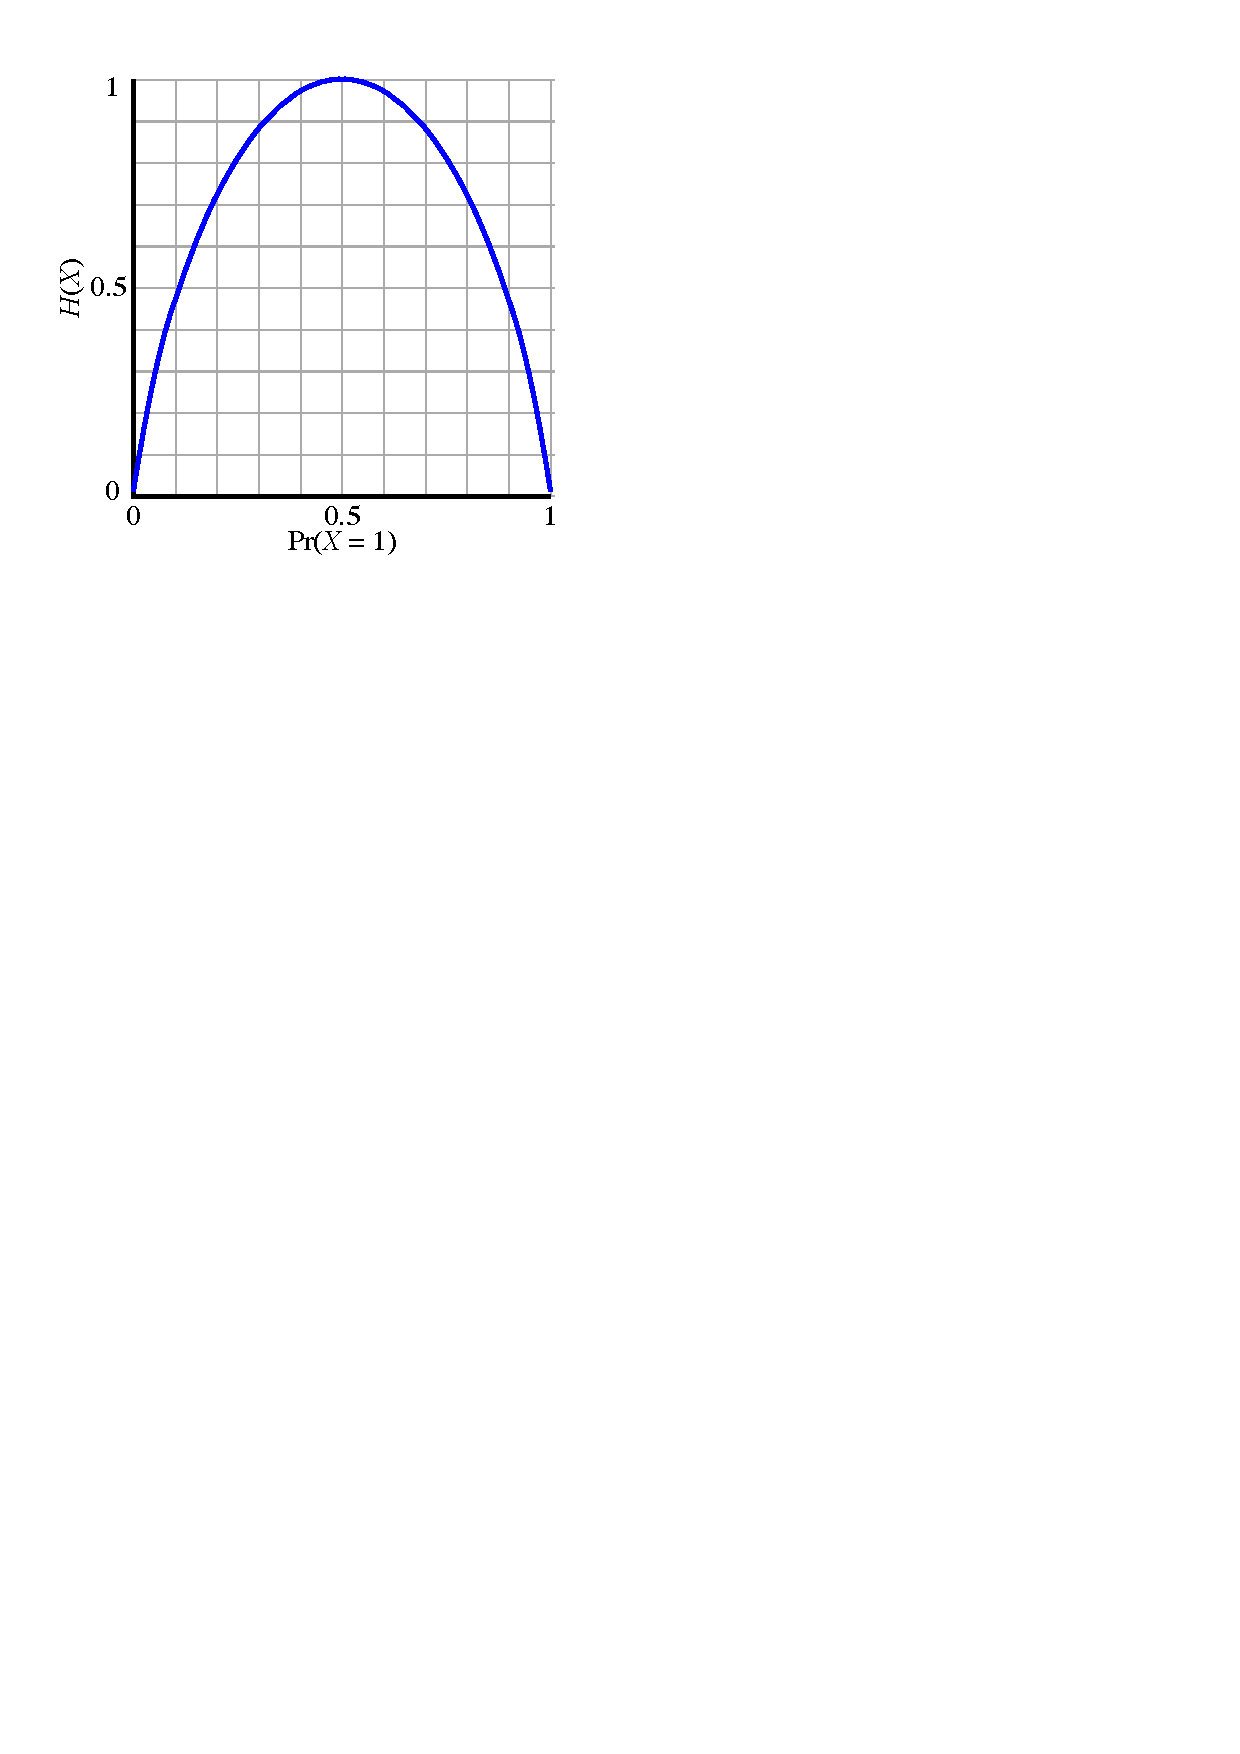
\includegraphics[width=1.3in]{figures/Binary_entropy_plot.pdf}
\end{center}
\end{minipage}

\underline{Canonical example:} \hfill \\  % TA lecture 1/7/2015. 
\begin{tabular}{ l | r }
  X & Y \\ \hline
  0 & 1 \\
  1 & 0 \\
  1 & 1 \\
\end{tabular}
\hfill \\
If you want to estimate entropy of X, you can use P(X=0).  \hfill \\
\begin{align*}
	H[X] &= -[\frac{1}{3} \log_2 \frac{1}{3} + \frac{2}{3} \log_2 \frac{2}{3}] \\
		& = \frac{1}{3} \log_2 3 + \frac{2}{3} \log_2 3 - \frac{2}{3} \log_2 2 \\
		&= \log_2 3 - \frac{2}{3} \approx 0.91
\end{align*}
This time H[X] = H[Y] because of symmetry.  \hfill \\

The discrete distribution with maximum entropy is the uniform distribution.  For K values of X, $H(X) = \log_2 K$ \hfill \\  % book pg 57
Conversely, the distribution with minimum entropy (which is zero) is any delta-function that puts all its mass on one state. Such a distribution has no uncertainty. 
\hfill \\

\subsection{Conditional Entropy}
If you don't know x:  (this is kind of an average).  \hfill \\
$H[Y \mid X=x] = -\sum\limits_y P(Y=y \mid X=x) \cdot \log_2 P(y \mid X=x)$   \hfill \\
 $H[Y \mid X=x] =  E[S(Y \mid X=x)]  $  \hfill \\
Note that we are summing over y because we are specifying x. \hfill \\
\hfill \\

For a particular value of X:  \hfill \\
$H[Y \mid X] = \sum\limits_x p(x) H[Y \mid X=x]$  \hfill \\
\hfill \\

Back to table above: 
\begin{align*}
	H[Y \mid X=0] &= ?  \\
	& \mbox{look only at X=0 in table.}  \\
	&= -[0 + 1 \log_2]  \\
\end{align*}
Now that you know X=0, entropy goes to 0.   \hfill \\  \hfill \\

$H[Y \mid X=1] = 1$: You know \textit{less} if you know X=1. \hfill \\ \hfill \\

Now use 
$H[Y \mid X] = \frac{1}{3}(0) + \frac{2}{3}(1) = 2/3$ \hfill \\
Given X, you know more.  Average our the more certain case and the less certain case.  \hfill \\  \hfill \\

Note:  $H[Y \mid X] \leq H[Y]$: knowing something can't make you know less. 

\subsection{Entropy and Information Gain}
\textbf{Information Gain} -  $IG(X) = H(Y) - H(Y \mid X)$ \hfill \\
Y is the node on top.  X are the nodes below.  He might have used lower case.  \hfill \\
\textbf{Class Example}: If $X_1$ is a node for a split, and you want to know the information gain for that node, you:
\begin{itemize}
	\item calculate entropy of the split.  Find Entropy of each branch of the split, and the fraction of points that were channeled to each split.  E.g. %http://courses.cs.washington.edu/courses/cse446/16wi/Slides/2_DecisionTrees_Part2.pdf
	\begin{align*}
		\{T, T, T, T, T, F\} & \rightarrow \{T, T, T, T\} \mbox{ (for } X_1=T), \{T, F\} \mbox{ (for } X_1=F) \\
				& \rightarrow P(X_1 = T) = 4/6, P(X_1=F) = 2/6 \\
				& \rightarrow H(X_1 = T) =  (1*\log_2 1 + 0*\log_2 0) = 0 \\
				& \rightarrow H(X_1 = F) =  \frac{2}{6} (\frac{1}{2} \log_2 \frac{1}{2} + \frac{1}{2} \log_2 \frac{1}{2})  \\
				& = 1 \mbox{ (uniform distribution)} \\
				H(Y|X_1)  =  - \frac{4}{6} & (1*\log_2 1 + 0*\log_2 0) - \frac{2}{6} (\frac{1}{2} \log_2 \frac{1}{2} + \frac{1}{2} \log_2 \frac{1}{2}) \\
							& = 2/6
	\end{align*}
	\item find the entropy of the unsplit data:  $\{T, T, T, T, T, F\} \rightarrow -(5/6) \log_2(5/6) - (1/6) \log_2(1/6) = 0.65$  % check w/ google: -(5/6)*log_2(5/6) - (1/6)*log_2(1/6) == 0.65. 
	\item subtract the weighted average of the split entropies from the original: $IG(X_1) = H(Y) - H(Y|X_1) = 0.65 - 0.33$
\end{itemize}


%\textbf{Conditional Information Gain}:    \hfill \\ %$H(y|x) = -\sum P(y|x) log_2$ 
  \hfill \\

\begin{itemize}
	\item Low uncertainty $\leftrightarrow$ Low entropy.
	\item Lowering entropy $\leftrightarrow$ More information gain. 
\end{itemize}


\subsection{Bits}
If you use log base 2 for entropy, the resulting units are called bits (short for binary digits). \hfill \\ % book pg 57
How many things can you encode in 15 bits? $2^{25}$.  \hfill \\  % 1/11/2015 Lecture


\subsection{Common notation}
\textbf{semicolon versus $|$ in probabilities}: \hfill \\
E.g. $P(X ; \theta)$ vs $P(X | \theta)$

$|$ is for random variables and $;$ is for parameters.  

Andrew Ng verbalizes the semicolon as "parameterized by."  
So $f(x ; \theta)$ would be spoken as "f of x parameterized by theta"
	






\section{Decison Trees}
\smallskip \hrule height 2pt \smallskip



\section{Maximum Likelihood \& Maximum a Posteriori}
\smallskip \hrule height 2pt \smallskip

\underline{Vocab}
\begin{itemize}
	\item\textbf{likelihood}: the probability of the data given a parameter.  E.g. $P(D | \theta)$ (for discrete like Binomial).  
	Need not a pdf; need not be normalized.   %  http://www.robots.ox.ac.uk/~az/lectures/est/lect34.pdf  + Erick
 	\item \textbf{log-likelihood}: lower-case: $l(\theta|x) = \log L(\theta | x)$
	\item \textbf{MLE}: Maximum Likelihood Estimation. 
	\item \textbf{PAC}: Probability Approximately Correct. 
\end{itemize}

\underline{ML}: Maximum Likelihood \hfill \\
 \hfill \\
 
\underline{MLE}: Maximum Likelihood Estimation \hfill \\
Choose $\theta$ to maximize probability of D. \hfill \\
Set derivative of \_\_ to zero and solve.  If function is multivariate, set each partial derivative to zero and solve. \hfill \\
$\hat{\theta} = \argmax_\theta P(D | \theta) = \argmax_\theta \ln P(D | \theta) $ \hfill \\
Note we are using $\ln$, not $\log_2$ as we did for entropy above.  Want it to cancel exponents now. 
 \hfill \\
 
\hfill \\
\underline{Binomial Distribution} \hfill \\
Assumes i.i.d: $D=\{x_i | i=1 \dots n\}, P(D | \theta) = \prod_i P(x_i \mid \theta)$. \hfill \\
Likelihood function: $P(D | \theta) = \theta^{\alpha_H} (1-\theta)^{\alpha_T}$  \hfill \\
P(heads) = $\theta$, P(tails) = $1 - \theta$ \hfill \\
\begin{align*} 
	\hat{\theta} &= \argmax_\theta \ln P(D| \theta) \\
	 	 &= \argmax_\theta \ln \theta*{\alpha H}(1-\theta)^{\alpha T}
\end{align*}
Find optimal theta by setting the derivative to zero: 
\begin{align*} 
	\frac{d}{d\theta} \ln P(D| \theta) &= \frac{d}{d\theta}  \ln \theta*{\alpha H}(1-\theta)^{\alpha T} \\
	 	 &= \argmax_\theta \ln \theta*{\alpha H}(1-\theta)^{\alpha T} \\
		 & = \dots = \frac{\alpha_H}{\alpha_H  + \alpha_T}
\end{align*}

For Binomial, there is exponential decay in uncertainty with \# of observations.  % slide 7 at http://courses.cs.washington.edu/courses/cse446/16wi/Slides/3_PointEstimation.pdf
You can also find the probability that you are approximately correct (see \href{http://courses.cs.washington.edu/courses/cse446/16wi/Slides/3_PointEstimation.pdf}{notes}).  \hfill \\
$P(|\widehat{\theta} = \theta*| \geq \epsilon) \leq 2e^{-2N\epsilon^2}$.  Can calculate N (\# of flips) to have error less than $\epsilon$ with probability of being incorrect $\delta$.  Your sensitivity depends on your problem; error on stock market data might cost billions. 

What if you had prior beliefs?  Use MAP instead of MLE.



\section{Bayesian Learning}
\smallskip \hrule height 2pt \smallskip

Rather than estimating a single $\theta$, we obtain a  distribution over possible values of $\theta$.

For small sample size, prior is important! 

Use Bayes' Rule:
$ \displaystyle P(\theta | D) = \frac{P(D | \theta) P(\theta)}{P(D)}$
\begin{itemize}
	\item \textbf{Posterior}: $P(\theta | D)$
	\item \textbf{Data Likelihood}: $P(D | \theta) $
	\item \textbf{Prior}: $P(\theta)$
	\item \textbf{normalization}: $P(D)$
\end{itemize}
Or equivalently, $P(\theta | D) \propto P(D | \theta) P(\theta)$

If you have a uniform prior, you just do MLE.  \hfill \\
$P(\theta) \propto 1 \rightarrow P(\theta | D) \propto P(D | \theta)$

\underline{Vocab}
\begin{itemize}
	\item \textbf{prior}: 
	\item \textbf{prior distribution}: 
	\item \textbf{posterior}: 
	\item \textbf{posterior distribution}: 
	\item \textbf{MAP}:
\end{itemize}

\hfill \\
\underline{Thumbtack Problem}
\begin{itemize}
	\item use Binomial likelihood:  $P(D | \theta) = \theta^{\alpha_H} (1-\theta)^{\alpha_T}$
	\item To get a simple posterior form, use a conjugate prior.  Conjugate prior of Binomial is the Beta Distribution.  See \href{http://courses.cs.washington.edu/courses/cse446/16wi/Slides/3_PointEstimation.pdf}{slides} for math. 
	\item The Beta prior is equivalent to extra thumbtack flips.  As $N \rightarrow \infty$, the prior is �forgotten�.  But for small sample size, prior is important.  
\end{itemize}

If you are measuring a continuous variable, Gaussians are your friend. 

\section{Gaussians}
\smallskip \hrule height 2pt \smallskip

Properties of Gaussians: 
\begin{itemize} 
	\item Affine transformation (multiplying by a scalar and adding a constant) are Gaussian.
		If X $\sim$ N($\mu$,$\sigma^2$) and Y = aX + b, then Y $\sim$ N($a\mu+b, a^2\sigma^2$) 
  	\item Sum of Gaussians is Gaussian.  
			If X $\sim$ N($\mu_X, \sigma^2_X$), 
			Y $\sim$ N($\mu_Y, \sigma^2_Y$), 
			and Z = X+Y, then 
			Z $\sim$ N($\mu_X+\mu_Y, \sigma_X^2 +\sigma_Y^2$)
	\item  Easy to differentiate.
\end{itemize}

Learn a Gaussian: $P(x | \mu, \sigma) = \frac{1}{\sigma \sqrt{2 \pi}}e^\frac{-(x-\mu)^2}{2\sigma^2}$. \hfill \\
MLE for Gaussian: Prob of i.i.d. samples D = $\{x_1, \dots, x_N\}$:  \hfill \\
$\displaystyle  P(D|\mu, \sigma) = ( \frac{1}{\sigma \sqrt{2 \pi}})^N \prod_{i=1}^N e^\frac{-(x_i-\mu)^2}{2\sigma^2}$.   \hfill \\
Note: it is \underline{not} $P(\mu, \sigma | D)$, like I thought in class.  \hfill \\
Find $\mu_{MLE}$, $\sigma_{MLE} = \argmax_{\mu, \sigma} P(D | \mu, \sigma)$.  \hfill \\

Log-likelihood:  $ \displaystyle \ln P(D | \mu, \sigma) = \ln[\mbox{thing above}] = -N \ln \sigma \sqrt{2\pi} - \sum_{i=1}^N \frac{(x_i - \mu)^2}{2\sigma^2}$.  \hfill \\
Differentiate w.r.t. $\mu$ and set = 0.  End up with $ \displaystyle \widehat{\mu} = \frac{1}{N} \sum_{i=1}^N x_i$.  \hfill \\
Differentiate w.r.t. $\sigma$ and set = 0.  End up with $ \displaystyle \widehat{\sigma}^2_{MLE} = \frac{1}{N} \sum_{i=1}^N (x_i-\widehat{\mu})^2$.  \hfill \\
But actually, that leads to a biased estimate, so people actually use  $ \displaystyle \widehat{\sigma}^2_{unbiased} = \frac{1}{N-1} \sum_{i=1}^N (x_i-\widehat{\mu})^2$  \hfill \\

The conjugate priors: mean: use Gaussian prior:  $ \displaystyle  P(\mu | \nu, \lambda) = \frac{1}{\lambda \sqrt{2 \pi}}e^\frac{-(\mu - \nu)^2}{2\sigma^2} $.  (Instead of $\sigma$, use $\lambda$ and replace the $(x-\mu)^2$ with $(\mu - \nu)^2$).  \hfill \\
For variance: use Wishard Distribution:  

\section{Linear Regression}
\smallskip \hrule height 2pt \smallskip

The loss is $|| y - Xw ||^2 + \lambda || w ||^2$ \hfill \\
(this corresponds to the sum of squared error loss + L2 regularization)\hfill \\
\hfill \\

\underline{Ordinary Least Squares} \hfill \\

Notation:
\begin{itemize}
	\item \textbf{$x_i$}: an input data point.  \_\_ rows by \_\_ columns. 
	\item \textbf{$y_i$}: a predicted output
	\item \textbf{$\widehat{y_i}$}: a predicted output
	\item \textbf{$\widehat{y}$}: 
	\item \textbf{$w_k$}: weight k
	\item \textbf{$\bm{w}^*$}: the vector of weights found in regression.   
	\item \textbf{$f_k(x_i)$}
	\item \textbf{$t$}: what we want to regress against
	\item \textbf{$t_j$}: the output variable that you either have data for or are predicting. 
	\item \textbf{$t(\bm{x})$}: Data.  "Mapping from x to t(x)"
	\item \textbf{$H$}: $H = \{ h_1, \dots, h_K \}$.  Basis functions.  In the simplest case, they can just be the value of an input variable/feature or a constant (for bias).  
	\item \textbf{$L_2$}: The $L_2$.  Can appear as a loss function to describe the deviation from data or as a penalty.  
		% Erick clarification
	\item \textbf{$ || \widehat{w} ||_1$}: "$L_1$" penalty.  The "Manhattan distance".  Like traveling a, b in a pythagorean triangle.  $\sum |x_i|$
	\item \textbf{$ || \widehat{w} ||_2$}.  "$L_2$" penalty.  Euclidean length of a vector.  Like c in a pythagorean triangle.  $\sqrt{\sum |x_i|^2}$	
\end{itemize}

\underline{Vocab}:
\begin{itemize}
	\item \textbf {bias-variance tradeoff} - the problem of simultaneously minimizing two sources of error that prevent 
			supervised learning algorithms from generalizing beyond their training set.  % https://en.wikipedia.org/wiki/Bias%E2%80%93variance_tradeoff
			\begin{itemize}  
				\item The bias is error from erroneous assumptions in the learning algorithm. 
					High bias can cause an algorithm to miss the relevant relations between features 
					and target outputs (underfitting).
				\item The variance is error from sensitivity to small fluctuations in the training set. 
					High variance can cause overfitting: modeling the random noise in the training 
					data, rather than the intended outputs.
			\end{itemize}
	\item \textbf{basis function}
	\item \textbf{bias} (parameter): like the intercept in a linear equation.  The part that doesn't depend on the features. 
	\item \textbf{bias} (learning bias):  (?? "inductive bias" ??)  - 
	\item \textbf{hyperplane} - a plane, usually with more than 2 dimensions. 
	\item \textbf{input variable} - a.k.a. feature.  % https://en.wikipedia.org/wiki/Dependent_and_independent_variables
		E.g. a column like CEO salary for rows of data corresponding to different companies.
	\item \textbf{response variable} - synonyms: "dependent variable", "regressand", "predicted variable", "measured variable", "explained variable", "experimental variable", "responding variable", "outcome variable", and "output variable".   E.g. a predicted stock price.   
	\item \textbf{regularization} -  introducing additional information in order to solve an ill-posed problem or to prevent overfitting. 
	% https://en.wikipedia.org/wiki/Regularization_(mathematics)
	E.g. applying a penalty for large parameters in the model. 
	\item \textbf{ridge regression} - 
	\item \textbf{vector norm}: put in a vector and get out a number like length or size.  Real valued function of some sort of vector or matrix quantity. 
	\item \textbf{hyperparameters}: \hfill \\
	$\lambda$, not $w$.  Parameters that control your actual parameters.  \hfill \\ \hfill \\
	% Wrong?!?   Norm 1 and norm 2 are not "parameters".  $\dots$ model design.  \hfill \\
	% Wrong?!?   Different values of lambda won't change the complexity of the model.  \hfill \\

	% Erick definition:
	In Bayesian analysis, the parameters that don't touch the data.  
	Like the parameters for the prior on the prior.  
	Called the ridge regression $\lambda$ a hyperparameter, though this is a stretch in the terminology.  \hfill \\
	Class version: 
	\item \textbf{feature selection}: explicitly select features that can go into your model instead of throwing all features in. 
	\item \textbf{loss function}:  
		% wikipedia:
		 A function that maps an event or values of one or more variables onto a real number intuitively representing some 			"cost" associated with the event. 
		 An optimization problem seeks to minimize a loss function. \hfill \\
		% week 4 typed notes near bottom. 
		$\sum_j (t(x_j) - \sum w_i h(x_i))^2$. (least-squares error ($L_2$))  (??? = training error??)
	\item \textbf{training set error}:  *doesn't include the regularization penalty!*.  A.k.a. "training error".  
			Sum of squares error divided by the number of points.   See formula later. 
%	\item \textbf{training error}:  sononomous
\end{itemize}

\subsection{Ordinary Least Squares}
total error = $\displaystyle \sum_i (y_i-\hat{y_i})^2 = \sum_i(y_i - \sum_k w_k f_k(x_i))^2$ \hfill \\
$i$ is for each data point, $k$ is for each of the k basis functions. 

 \hfill \\ \hfill \\

Under the additional assumption that the errors be normally distributed, OLS is the maximum likelihood estimator. \hfill \\ % https://en.wikipedia.org/wiki/Ordinary_least_squares
?? Use words to describe what subset of regression in general this is.  What is ordinary? What are we limiting?  \hfill \\
 \hfill \\

The regression problem: \hfill \\
Given basis functions $\{ h_1, \dots, h_K \}$  with $h_i(\bf{x}) \in \mathbb{R}$,  \hfill \\
	find coefficients $\bm{w} = \{ w_1, \dots, w_k \}$.  \hfill \\%  
$t(\bm{x}) \approx \widehat{f}(\bm{x}) = \sum_i w_i h_i(\bm{x})$     \hfill \\  \hfill \\


This is called linear regression b/c it is linear in the parameters. 
We can still fit to nonlinear functions by using nonlinear basis functions;  $f_k \rightarrow  h_i$
Minimize the \textbf{residual squared error}: \hfill \\
$ \displaystyle \bm{w}* = \argmin_{\bm{w}}  \sum_j (t(\bm{x}_j) - \sum_i w_i h_i(\bm{x}_j))^2$  \hfill \\
$j$ for each data point, $i$ for the number of weights, which is the number of basis functions.  \hfill \\
\hfill \\  \hfill \\

For fitting a line in 2D space, your basis functions are $\{ h_1(x) = x, h_2(x) = 1 \}$.  $h_2(x)$ = 1 is the (constant) bias basis function.  The size of $w_2$ controls the effect in prediction.    \hfill \\  \hfill \\

To fit a parabola, your basis functions could be $\{ h_1(x) = x^2, h_2(x)=x, h_3(x)=1 \}$.   \hfill \\
Want a 2D parabola? Use $\{ h_1(x) = x_1^2, h_2(x)=x_2^2, h_3(x)=x_1 x_2, \dots \}$. \hfill \\
Can define any basis functions $h_i(\bm{x})$ for n-dimensional input $\bm{x} = <x_1, \dots, x_n>$
\hfill \\  \hfill \\

\underline{Linear in feature space vs linear in the parameter space}:  \hfill \\
When we want to fit a parabola, we are still using a function that is linear in \underline{parameter} space. 
The weight matrix is still all constants. 
When we use nonlinear basis functions, we are nonlinear in \underline{feature} space.  The basis functions may be transformations of the input parameters. 
 \hfill \\ \hfill \\

\subsection{Regression: matrix notation}
\begin{align*}
	\bm{w}* &= \argmin_w \sum_j(t(\bm{x}_j - \sum_i w_i h_i(\bm{x}_j))^2  \\
	\bm{w}* &= \argmin_w (\bm{Hw} -\bm{t})^T (\bm{Hw} -\bm{t})
\end{align*}
$  (\bm{Hw} -\bm{t})^T (\bm{Hw} -\bm{t})$ is the residual error.  
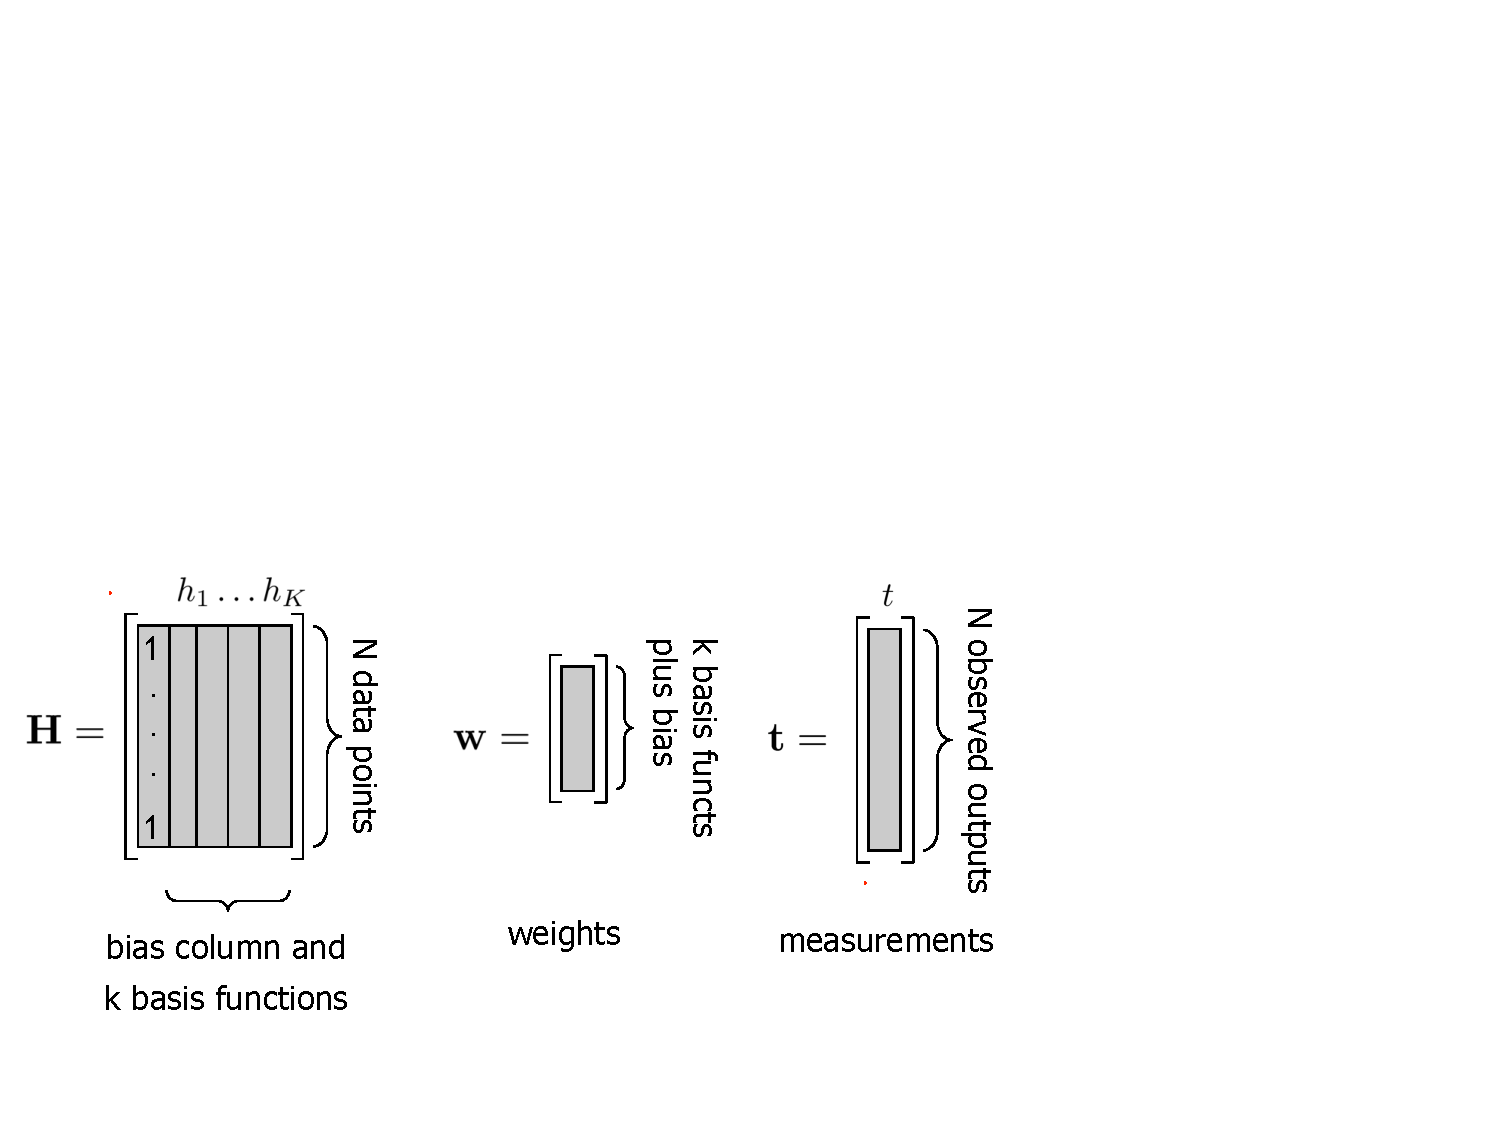
\includegraphics[width=3in]{figures/Least_squares_matricies.pdf}

\subsection{Regression: closed form solution}
 % derivation: http://courses.cs.washington.edu/courses/cse446/16wi/Slides/4_LinearRegression.pdf
\begin{align*}
	\bm{w}^* = \argmin_w (\bm{Hw} -\bm{t})^T (\bm{Hw} -\bm{t})  & \\
	\bm{F}(\bm{w}) =  \argmin_w (\bm{Hw} -\bm{t})^T (\bm{Hw} -\bm{t}) & \\
	\triangledown_{\bm{w}}\bm{F}(\bm{w}) = 0 \\
	2 \bm{H}^T (\bm{H}\bm{w}-\bm{t}) = 0  & \\
	(\bm{H}^T\bm{H}\bm{w}) - \bm{H}^T\bm{t} = 0 & \\
	\bm{w}^* = (\bm{H}^T\bm{H})^{-1}\bm{H}^T\bm{t} &
\end{align*}

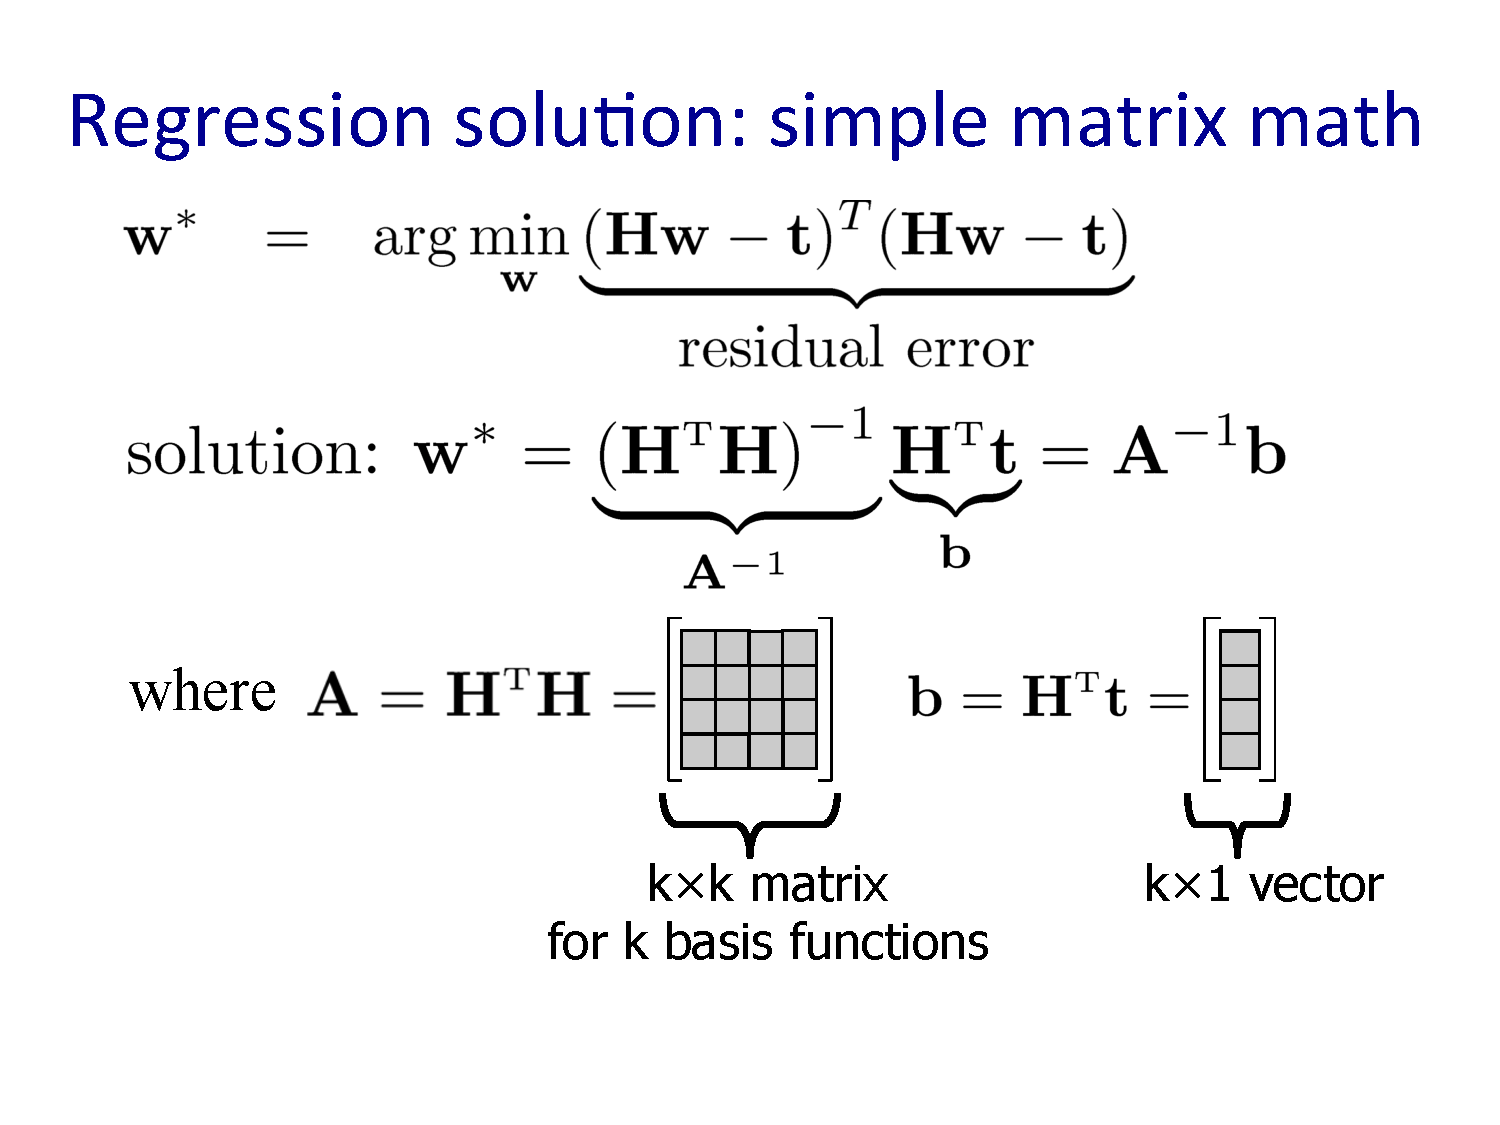
\includegraphics[width=3in]{figures/Regression_matrix_math.pdf}

Dimensions: 
\begin{itemize}
	\item $\bm{t}$:  N-dimensional  (N = \# of input data points) 
	\item $\bm{w}$: 
	\item $\bm{H}$: k + 1 by N.  N is \# of rows. 
\end{itemize}
\hfill \\

\subsubsection{Linear regression prediction is a linear function plus Gaussian noise}
%______TA e-mail 3/15________________________
\underline{Casual explanation:} \hfill \\
If we assume that our data $y_i$ is drawn from a linear function with some zero-mean Gaussian noise, i.e.

$$y_i = \sum_j w_j X_ij + \epsilon_i$$
(where $\epsilon_i$ is zero-mean gaussian noise drawn from Normal(0, $\sigma$)

Then we can show that the MLE estimates of $w_j$ are exactly the optimal weights obtained by minimizing the SSE: $\sum_i (y_i - w^T X_i)^2$

(note that the variance $\sigma$ actually doesn't matter for the derivation, you can just assume it's some positive number). \hfill \\ %%
\hfill \\
%______________________________
\underline{More formal explanation:} \hfill \\
We can model as linear combination of basis functions + noise $\epsilon$.  
It's safe to assume epsilon comes from Gaussian distribution.  \hfill \\

$t(\bm{x}) = \sum_i w_i h_i(\bm{x}) + \epsilon $ \hfill \\
Note: no $\mu$ because we set it to zero.  \hfill \\

We can learn $\bf{w}$ using MLE: 
$P(t | x, w, \sigma) = \frac{1}{\sigma \sqrt{2 \pi}} e^\frac{-[t - \sum_i w_i h_i(x)]^2}{2 \sigma^2}$
Take the log and maximize with respect to w:  (maximizing log-likelihood with respect to w) \hfill \\
$\displaystyle \ln P(D | \bm{w}, \sigma) = \ln(\frac{1}{\sigma \sqrt{2 \pi}})^N \prod_{j=1}^N e^\frac{-[t_j - \sum_i w_i h_i(x_j)]^2}{2 \sigma^2}$ \hfill \\
Now find the w that maximizes this: \hfill \\
$\argmax_w \ln(\frac{1}{\sigma \sqrt{2 \pi}})^N + \sum_{j=1}^N \frac{-[t_j - \sum_i w_i h_i(x_j)]^2}{2 \sigma^2}$ \hfill \\
the first term isn't impacted by $w$ so  \hfill \\
$= \argmax_w  \sum_{j=1}^N \frac{-[t_j - \sum_i w_i h_i(x_j)]^2}{2 \sigma^2}$ \hfill \\
switch to $\argmin_w$ when we divide by -1.  The numerator is constant.:  \hfill \\
$= \argmin_w  [t_j - \sum_i w_i h_i(x_j)]^2 $ \hfill \\

\textbf{Least-squares Linear Regression is MLE for Gaussians!!!}  \hfill \\ \hfill \\

If you have a polynomial you are fitting, how many basis functions are there (??)  \hfill \\ % asked Wed 1/27


\subsection{OLS Protocol (incomplete)}  \hfill \\
\begin{enumerate}
	\item Chose your basis functions $h_i$.  (Requires expertise).  Can be nonlinear, e.g. $x_1^2, \sin(x)$, etc. 
		\begin {itemize}
			\item 
				The number of parameters is len(H) + 1 (bias).  
				E.g. for fitting a parabola (formula $y = ax^2 + bx + c$), 
				you have 3 parameters: weights for basis functions $x$, $x^2$, and bias. 
				Typically the \# of basis functions is $<$ the \# of features.
		\end {itemize}
	\item Chose a regularization method so your weights don't get too big.  (see below)
	\item Plug them in to regression to get the weights ($w_i$s).  (Form the sum (residual squared error + regularization) that you want to minimize, then minimize.)    
	\item Make sure your weights aren't too big. 
	
\end{enumerate}

\subsection{Regularization in Linear Regression}  \hfill \\
You need to regularize to prevent parameters from growing too large.  
Both of these were built from the same set of basis functions; the right one is clearly over-fit. \hfill \\
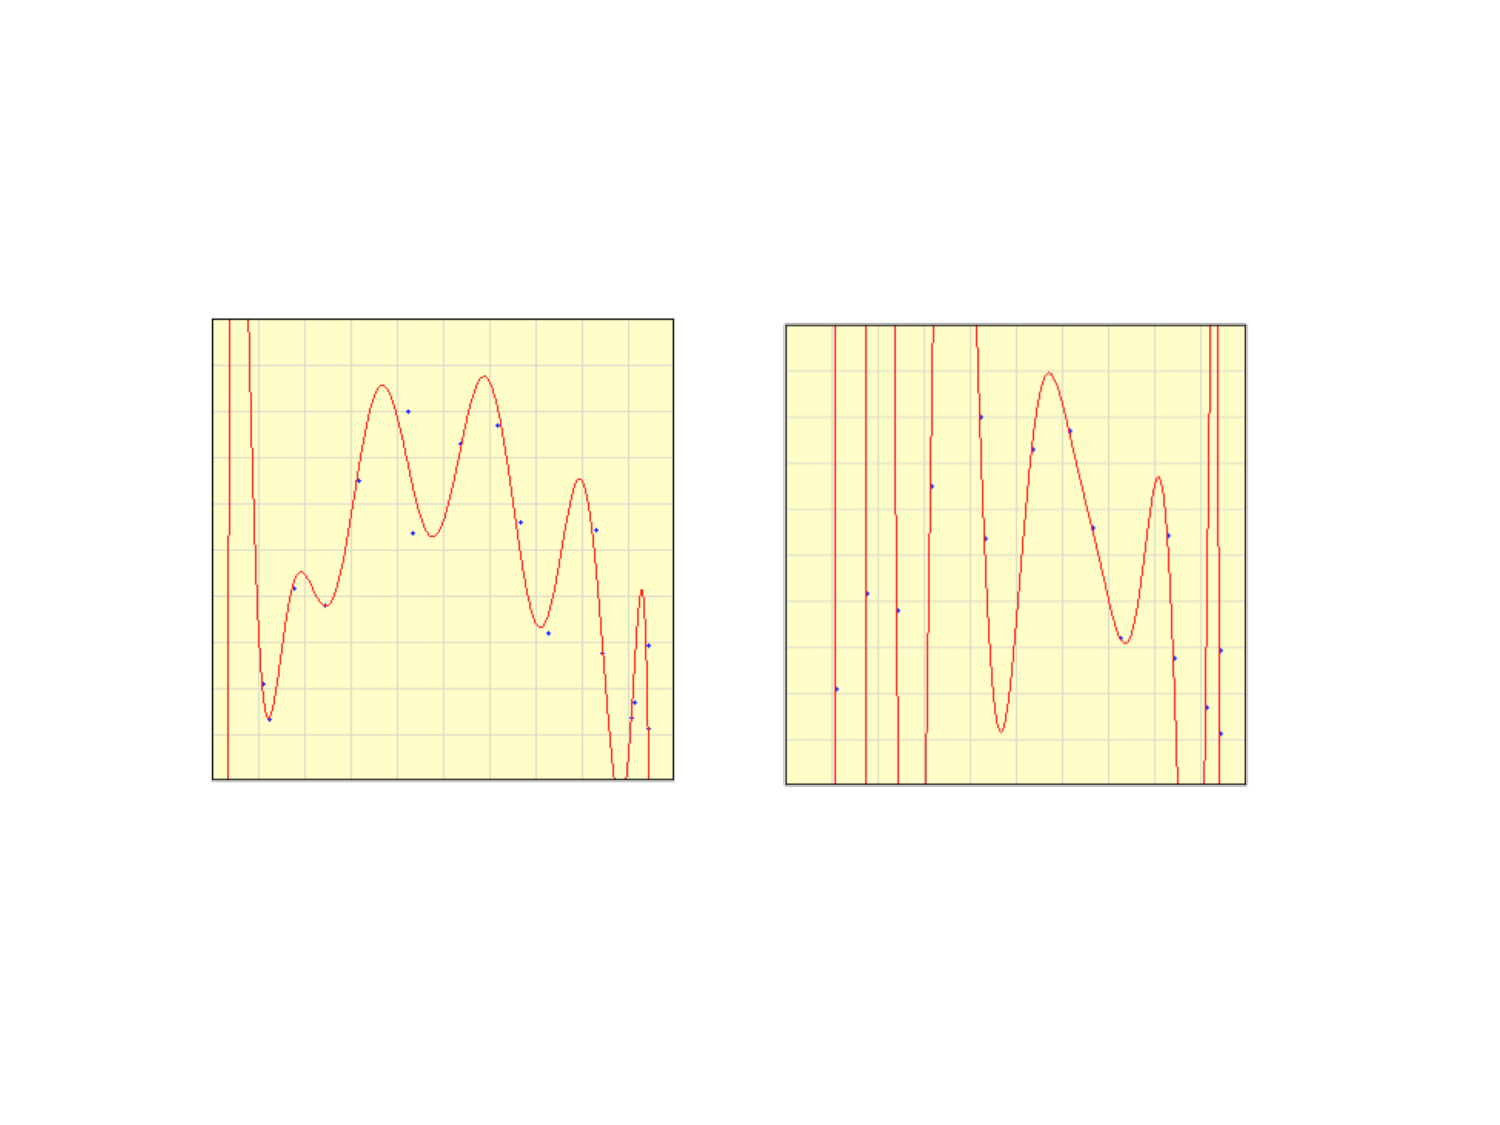
\includegraphics[width=1.2in]{figures/need_to_regularize.pdf}

\subsubsection{Ridge Regression}  \hfill \\
Ridge Regression is the most famous form of linear regression
Here is our old "ordinary" least squares objective function:   \hfill \\
$\displaystyle \widehat{w} = \argmin_w \sum_{j=1}^N [t(x_j) - (w_0 + \sum_{i=1}^k w_i h_i(x_j))]^2$   \hfill \\
It is the same as the previous ones but $i=0$ is pulled out.    \hfill \\
Now for ridge regression, we use that same notation.  \hfill \\
And we add a penalty term that isn't applied to the bias feature:
\begin{align*}
	\widehat{w}_{ridge} &= \argmin_w \sum_{j=1}^N [t(x_j) - (w_0 + \sum_{i=1}^k w_i h_i(x_j))]^2 + \lambda \sum_{i=1}^k w_i^2   \\
	&= \argmin_w (\bm{H}\bm{w} - \bm{t})^T(\bm{H}\bm{w}-\bm{t}) + \lambda \bm{w}^T I_{0+k} \bm{w}
\end{align*}
That $I_{0+k}$ matrix is this: 
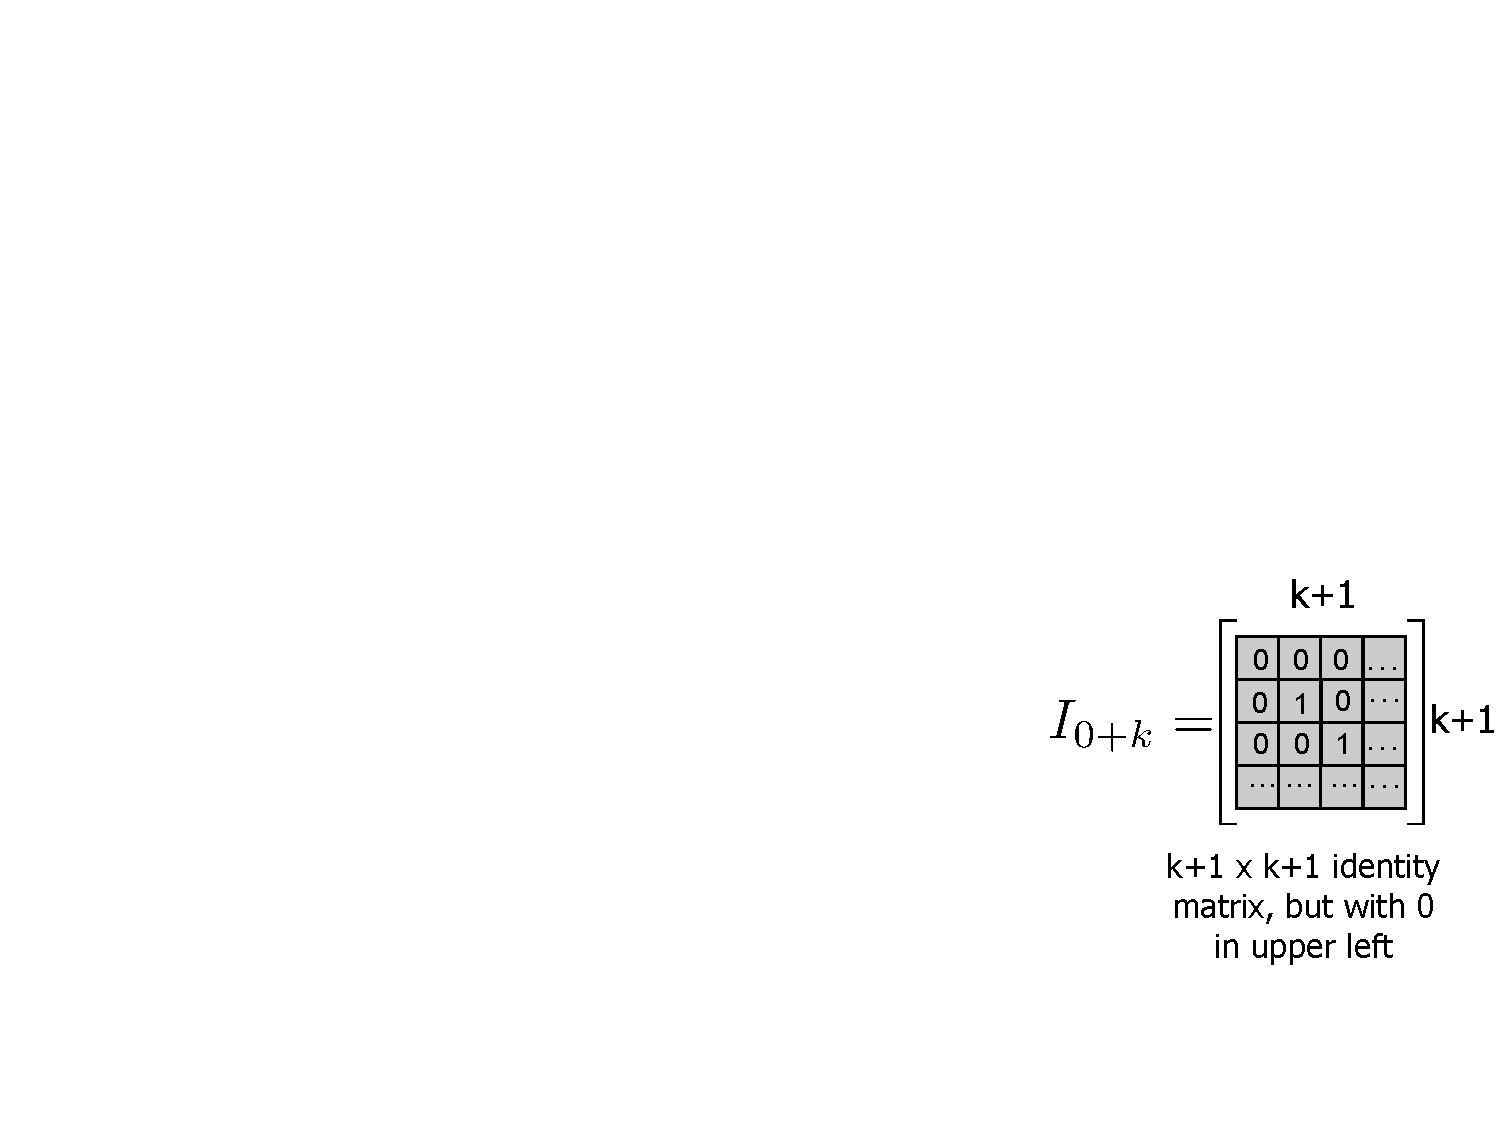
\includegraphics[width=1.0in]{figures/ridge_identity_matrix_with_zero.pdf}  \hfill \\
% Erick hasn't seen this notation.
Allows you to multiply the whole weight array without getting the bias term in there. 

Note: $W^TW$ is $w_i^2$ or $|| w_i ||^2$ 

A similar derivation leads to a closed form solution:  \hfill \\
% http://courses.cs.washington.edu/courses/cse446/16wi/Slides/4_LinearRegression.pdf 
$w_{ridge}^* = (\bm{H}^T\bm{H} + \lambda I_{0+k})^{-1}\bm{H}^T\bm{t}$ \hfill \\
(Recall that un-regularized regression was $w^* = (\bm{H}^T\bm{H})^{-1}\bm{H}^T\bm{t}$).  \hfill \\   \hfill \\

How do you chose how large $\lambda$ is? \hfill \\
* As $\lambda \rightarrow 0$, becomes same as MLE: unregularized.  Large magnitudes of coefficients. \hfill \\
* As $\lambda \rightarrow \infty$, all weights become 0.  \hfill \\   \hfill \\

\subsubsection{Experiment cycle}
\begin{enumerate}
	\item select a hypothesis $f$ to best match the training set.  
		(??) Is this the same as choosing your basis functions (?)
	\item isolate a held-out data set if you have enough data, or do K-fold cross-validation if not enough data. 
	\begin{itemize}
		\item tune hyperparameters ($\lambda$) on the held-out set or via cross-validation.  
			(Try many values of $\lambda$ and chose the best one.) 
		\item You can use the same held-out data set each time if that set is big.  
		\item If doing K-fold, divide the data into k subsets.  
				Repeatedly train on k-1 and test on the remaining one.  
				Average the results. 
		\item find the $w$ that minimizes the error.  
			(Do so by taking the derivative and setting = 0); 
			see ridge regression notes. 
	\end{itemize}
	\item Select basis functions
\end{enumerate}

\subsection{Regularization options: Ridge \& Lasso}  \hfill \\
Ridge: 
\begin{itemize}
	\item $ \displaystyle \widehat{w}_{ridge} = \argmin_w \sum_{j=1}^N [t(x_j) - (w_0 + \sum_{i=1}^k w_i h_i(x_j))]^2 + \lambda \sum_{i=1}^k w_i^2   $ 
	\item $L_2$ penalty.  ("$L_2$ norm of $\bm{w}$).  
		Large distances get penalized more.  $Y = x^2$: 
		don't want errors to cancel each other; differentiable. 
\end{itemize}
Lasso: \hfill \\
\begin{itemize}
	\item$ \displaystyle \widehat{w}_{ridge} = \argmin_w \sum_{j=1}^N [t(x_j) - (w_0 + \sum_{i=1}^k w_i h_i(x_j))]^2 + \lambda \sum_{i=1}^k |w_i|   $ 
	\item L1 penalty: linear penalty pushes more weights to zero.  Allows for a type of feature selection.  But it is not differentiable and there is no closed form solution. 
	\item L1 is absolute value: don't need to square it. 
	\item Lasso may be more useful when you have too many features for the amount of data you get.  
		Example: 100k parameters about companies to predict stock prices but only 100 data points.  
		Could tune lambda until you have about 100 nonzero weights. 
\end{itemize}

Your chose of penalty has huge effects on the algorithm! \hfill \\
Sometimes $L_1$ will do better than $L_2$ and vice versa, but usually $L_2$ is more powerful than $L_1$. \hfill \\
Would be better to use a combination of the penalties than to first reduce the number of features with $L_2$ before applying $L_1$.    \hfill \\
You can generate a lot of basis functions and use $L_1$ to chose the good ones. \hfill \\
\hfill \\

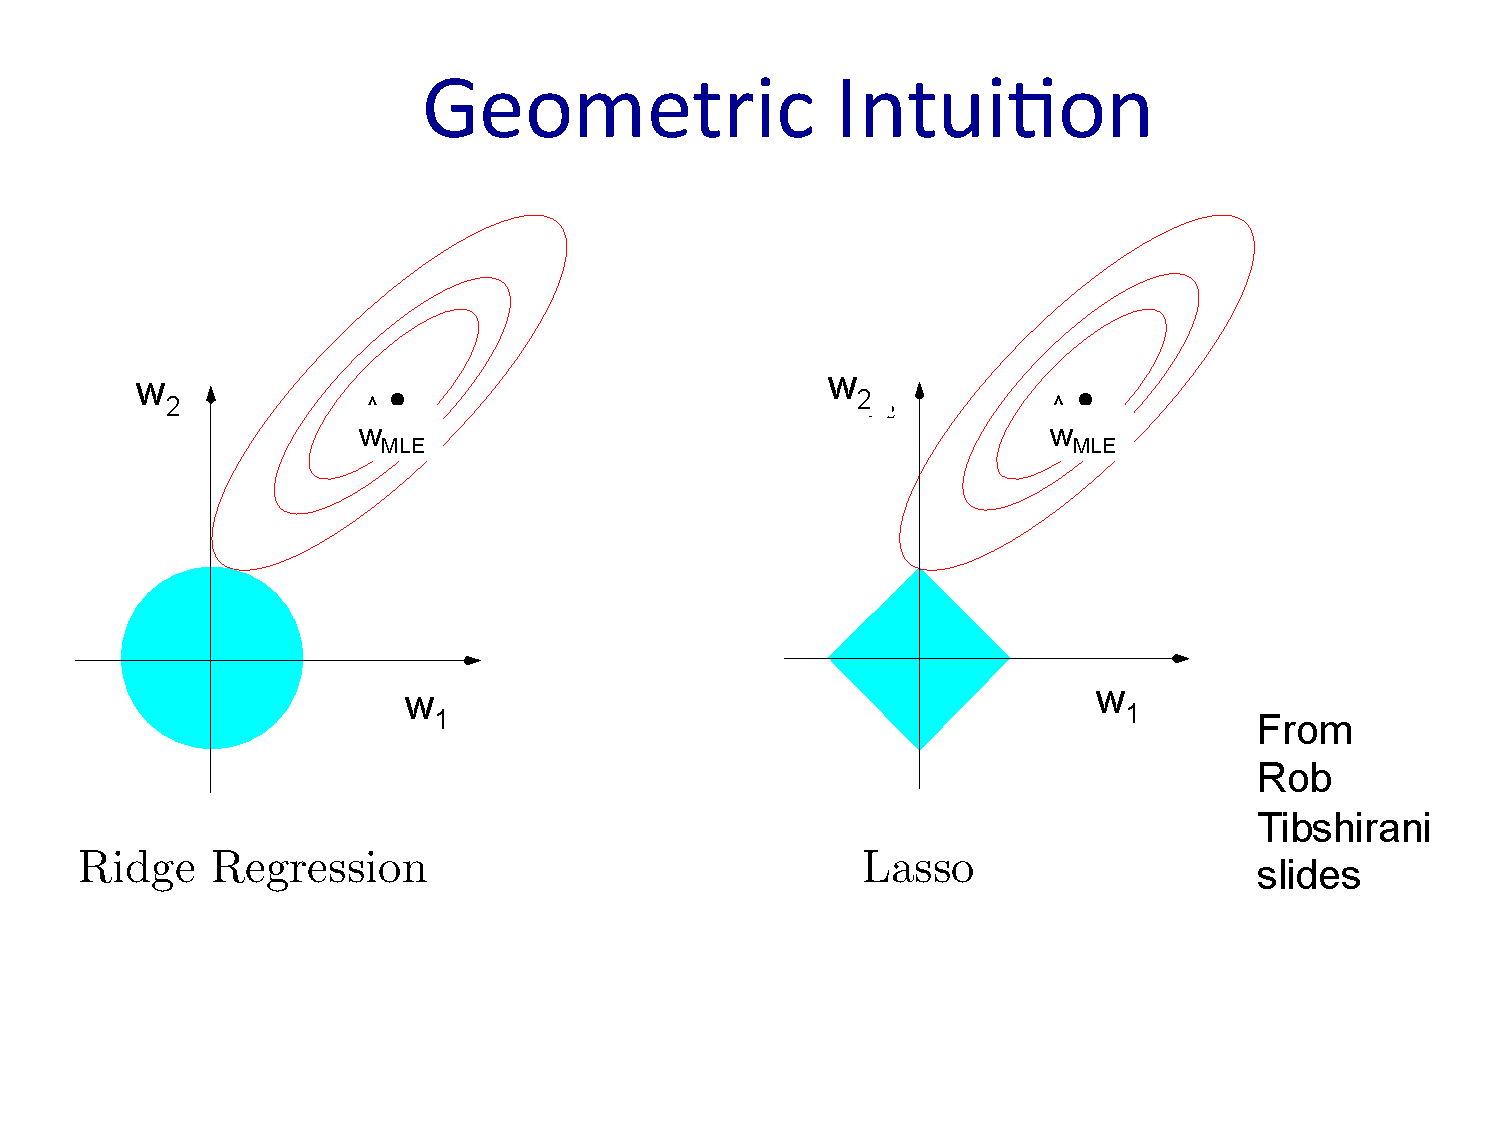
\includegraphics[width=3in]{figures/lasso_and_ridge_geometry.pdf}

This figure shows: 
\begin{itemize}
	\item The contour lines represent the maximum likelihood of the vector of weights.  
		All points on the contour have equal likelihood.
	\item The two axes represent different parameters for two of the weights.  (regression coefficients)
	\item Circles are characteristic of ridge regression (with L2 penalty): Penalty = the magnitude of the vector.
	\item Shapes that are pointy on the axes are characteristic of Lasso (with L1 penalty): the vector components get added. 
	\item Where the likelihood function touches in this $w_1, w_2$ space represents the coefficients of the weights.
		For Ridge Regression, we see that small but nonzero values of the coefficients can be obtained.
		For Lasso Regression, the curves are most likely to touch the diamond on the axes, 
		resulting in coefficients that are truly zero. 
\end{itemize} 

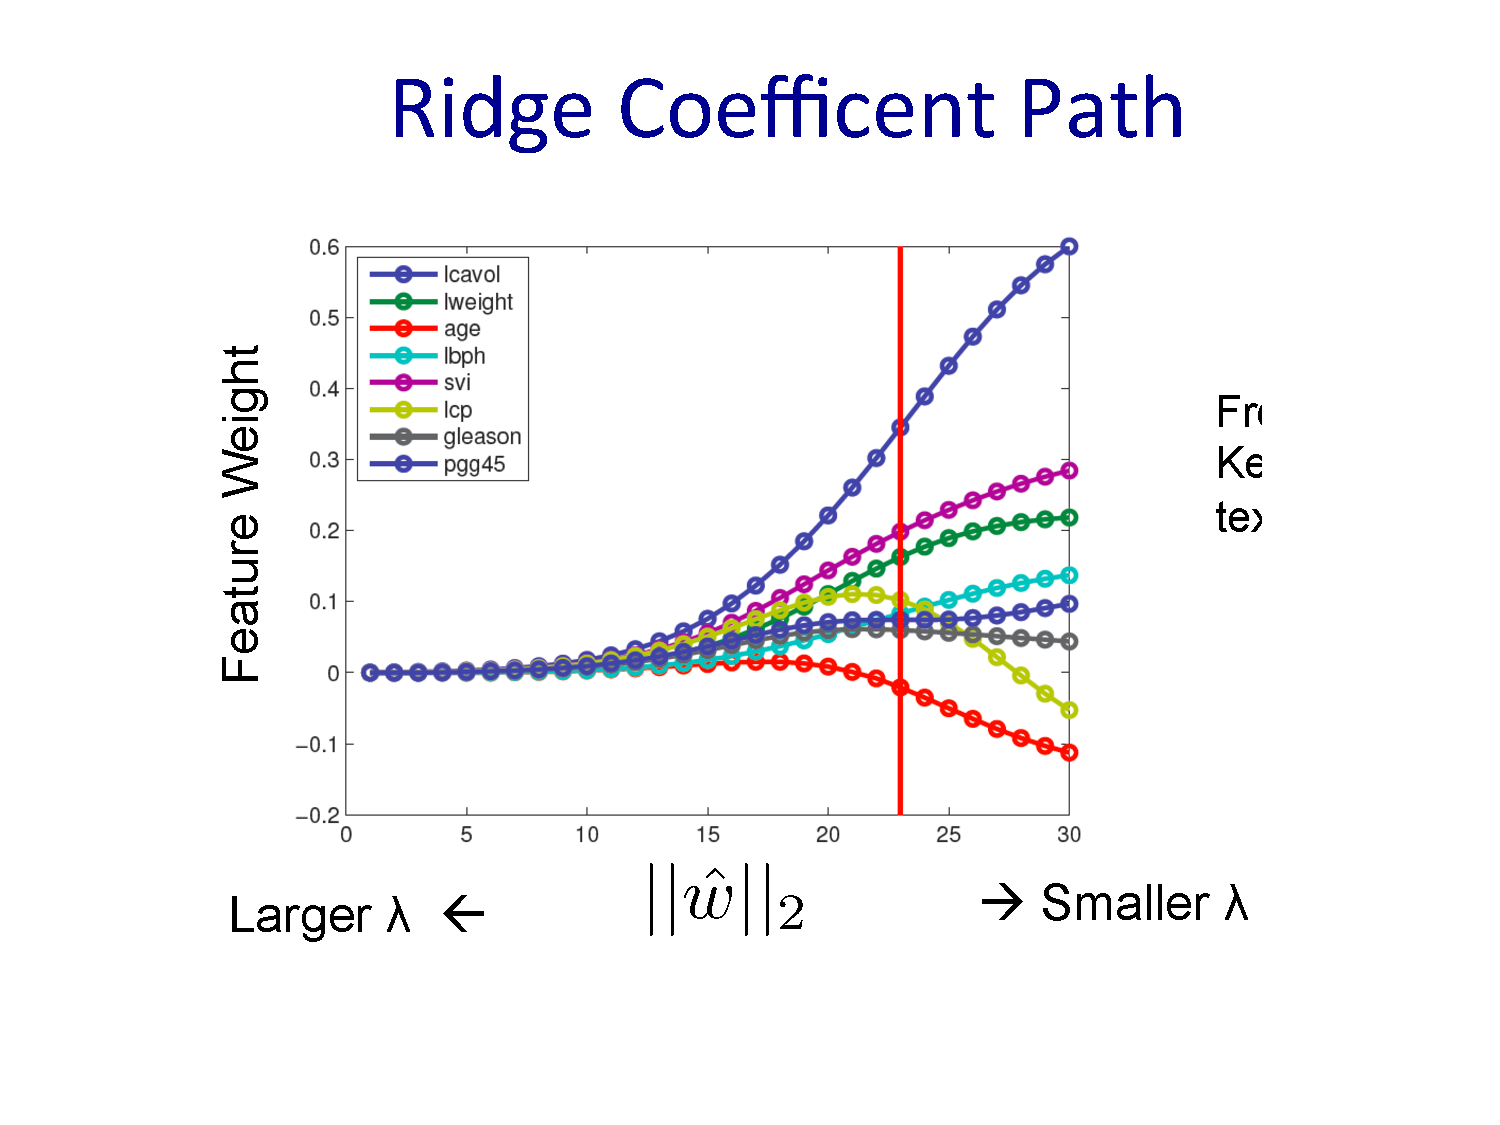
\includegraphics[width=1.8in]{figures/lambda_with_w2.pdf}  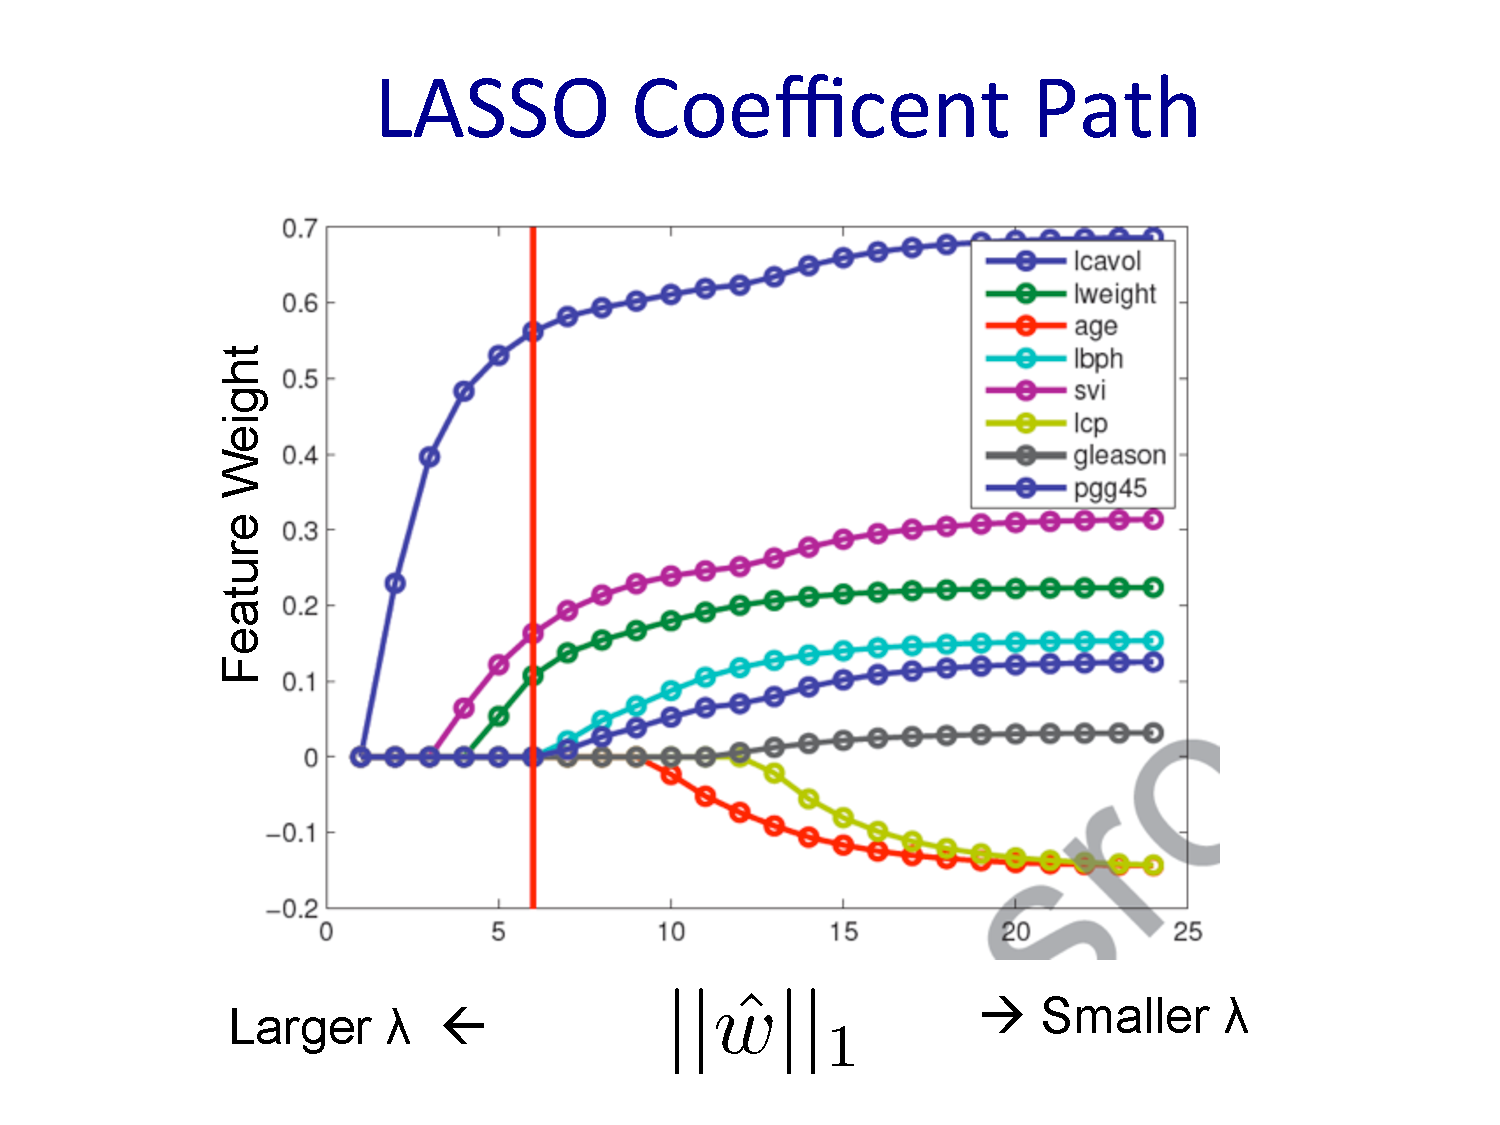
\includegraphics[width=1.6in]{figures/lambda_with_w1.pdf}
Don't compare coefficient magnitudes at given $\lambda$s, 
but do note that for Ridge the gradually come away from the zero axis and in Lasso they are zero until they pop out.   \hfill \\ \hfill \\

\subsection{Bias-Variance Tradeoff}
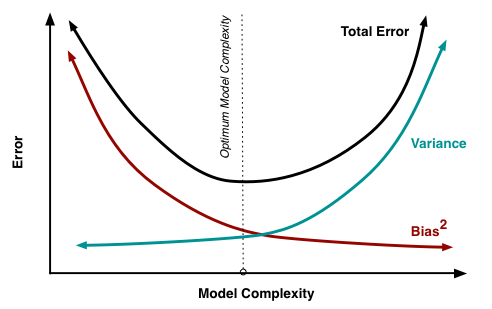
\includegraphics[width=2.0in]{figures/biasvariance.png} 

Your choice of hypothesis class (e.g. degree of polynomial) introduces learning bias.  \hfill \\
The more complex the model, the more the \_\_\_\_ set accuracy goes down  \hfill \\  % had "training" with ?
\textbf{A more complex class } $\rightarrow$ less bias and more variance.   \hfill \\ \hfill \\

From https://www.youtube.com/watch?v=Rm6s6gmLTdg: hfill \\
High bias = inability to represent the true function in the class of functions we are willing to tolerate.
Pulls us to a particular function or class of functions regardless of the data.
Can be from looking only at a specific type of function, or by having strong regularization  \hfill \\
High variance = extremely dependent on the exact data they were trained on.
Might fit the data well, but may do poorly on a different data self.  \hfill \\


From Wikipedia: \hfill \\  % https://en.wikipedia.org/wiki/Bias%E2%80%93variance_tradeoff
Ideally, one wants to choose a model that both accurately captures the regularities in its training data, 
but also generalizes well to unseen data. Unfortunately, it is typically impossible to do both simultaneously. 
High-variance learning methods may be able to represent their training set well, but are at risk of overfitting 
to noisy or unrepresentative training data. 
In contrast, algorithms with high bias typically produce simpler models that don't tend to overfit, 
but may underfit their training data, failing to capture important regularities. \hfill \\  \hfill \\

Models with low bias are usually more complex (e.g. higher-order regression polynomials), 
enabling them to represent the training set more accurately. 
In the process, however, they may also represent a large noise component in the training set, 
making their predictions less accurate - despite their added complexity. 
In contrast, models with higher bias tend to be relatively simple (low-order or even linear regression polynomials), 
but may produce lower variance predictions when applied beyond the training set. \hfill \\ \hfill \\

Adding features (predictors) tends to decrease bias, at the expense of introducing additional variance.   \hfill \\
\hfill \\

Solutions:
\begin{itemize}
	\item Dimensionality reduction and feature selection can decrease variance by simplifying models. 
	\item Similarly, a larger training set tends to decrease variance. 
	\item Use tunable modeling parameters such as applying more significant regularization.
\end{itemize}

\textbf{If held-out is too small, we can end up over-fitting.}


\hfill \\  \hfill \\

\subsection{Error Definitions}

\underline{True ("Prediction") Error}:   \hfill \\
Since the training set error can be a poor measure of the "quality" of the solution, we can use prediction error ("true error").  
The error over all possibilities.   Instead of sum, take expectation. 
\begin{align*}
	error_{true}(\bm{w}) &= E_X[(t(\bm{x_j})-\sum_{i} w_i h_i(\bm{x_j}))^2] \\
		& \mbox{Gold Standard:} \\
	error_{true}(\bm{w}) &= \int_x (t(\bm{x_j})-\sum_{i} w_i h_i(\bm{x_j}))^2 p(\bm{x}) d\bm{x}
\end{align*}

% TA 3/15/2016:
$p(x)$ is assumed to be the "true" distribution of the data, which we don't actually know. 

How to get $p(\bm{x})$?  Need to know the true distribution of the data (?).  
You almost never know how to compute $p(x)$.
And, the integral is a very big sum. \hfill \\  \hfill \\

% Find $p(x)$ using monte-carlo integration. \hfill \\

% TA 3/15/2016:
To do this, you need to split your data into training and test set. 
If we have a dataset which is randomly sampled from $p(x)$, which we assume our data is, we can estimate the true error using the average of the samples. 
Since we train on our training set, the error might be a bad estimate of the true error (we're biased to decrease the error), so we use a separate hold-out testing set to approximate the true error in instead.

Sample a set of i.i.d. points  $\{ \bm{x}_1, \dots, \bm{x}_M \}$ from $p(x)$.   \hfill \\
Approximate the integral with the sample average:
$$ error_{true}(\bm{w}) \approx \frac{1}{M} \sum_{j=1}^M \left( t(\bm{x}_j - \sum_i w_i h_i(\bm{x}_j) \right) $$
That is the sampling approximation of the predicted error: \hfill \\
That leads to a fair approximation.   \hfill \\

\hfill \\  \hfill \\

The true prediction error is the expectation over \textbf{future} test cases you don't have.  
Since you don't have the x values, you go to probability. 
Pick a point from the distribution, and calculate the \_\_\_\_\_.     \hfill \\  \hfill \\

Don't use the training data to predict true error; you've already trained to that data!  You would have too optimistic of a prediction for true error. 

Prediction error is high when the model is too simple \underline{and} too complex, unlike training set error which only penalizes too simple.  \hfill \\
\hfill \\

\underline{Training Set Error}:  \textbf{optimistically biased}  (a.k.a. training error) \hfill \\
$\displaystyle  error_{train}(\bm{w}) = \frac{1}{N_{train}} \sum_{j=1}^{N_{train}}(t(\bm{x_j})-\sum_{i} w_i h_i(\bm{x_j}))^2$ \hfill \\
Decreases exponentially with model complexity.   \hfill \\
\textbf{Training error is a poor prediction of prediction error!} \hfill \\
You expect to see training error to decrease with complexity, but that doesn't mean you have a good solution!  \hfill \\
\hfill \\  \hfill \\
% http://courses.cs.washington.edu/courses/cse446/16wi/Slides/4_LinearRegression.pdf


\underline{Test Error}: (our final measure)  \hfill \\
Uses the same formula as prediction error, except that we have never observed the test data.  See formula below. 
We expect the true error to be smile shaped if the x-axis is model-complexity. 
\hfill \\ \hfill \\

\underline{\textbf{Testing is for the user of your algorithm. }}
The user doesn't care about the values in your model.  They just care about how well it works.  
 They dont' care about the value of your hyperparameters. 


\subsubsection{Effects of $\lambda$ value on model}
% week 4 typed notes. 
 \begin{itemize}
 	\item high lambda $\rightarrow$ simple model $\rightarrow$ lots of zeros $\rightarrow$ high error. 
	\item with lambda = 0 $\rightarrow$ converges ridge regression to regular regression. 
	\item with enough traiing data and lambda = 0, we expect overfitting $\rightarrow$ small training error. 
\end{itemize}

\subsubsection{Choosing $\lambda$}
How to find lambdas? 
\begin{itemize}
	\item try a bunch and find which does best on the held out data set.  
		Can't touch test data, even w/ stick so use held-out set. 
	\item Do k-fold cross validation to pick the lambda that gives minimum error. \hfill \\
		Average over the loss curves Loss($fold_i$, $\lambda$) \hfill \\ 
		Minimum error = lowest loss on the hold-out set (the curve should look U shaped, so you just find the bottom of the U).  \hfill \\
		May not find the bottom-of-the-U shape lambda.    \hfill \\
		But it is ok to be off a bit; the red U might be pretty flat at the bottoms. \hfill \\
\end{itemize}		
This use of the held-out data doesn't count as training.  
Lambda is fixed each time, and we train separately. 
Training on training data, just watching the number on the held-out set. \hfill \\
\textbf{The model's parameters are not determined by the held-out data} \hfill \\
\hfill \\

How do you chose the range of lambda? (practical solution) 
\begin{itemize}
	\item You are limited to a grid search over values of lambda. 
	\item You need a strategy for sweeping that space.   
		Could do a "binary search", or something like a gradient search: 
		take a step until we screw it up, and step back smaller.   
		If it gets worse, you take a smaller step.
	\item From your loss, take the value of your loss (compute it).  \hfill \\
		Loss = $(t(x) - \sum w_i h(x_i))^2$  
        		\textbf{"You should be able to find loss given w}
            	Can compute norm of W, too.  
		If your loss is on the order of 1000 and your norm is on the order of 1, you can use these for defining search space.
                	Firs try lamba = 1, 10, 100, 1000.  
		Find the best from there then explore around there.
		If 100 was good, try 200, etc.   
		You just want to know in which order the loss function is going to appear. 
\end{itemize}

\subsubsection{How to handle error calculations:}
Given a dataset, randomly split it into two parts:  \hfill \\
* training data: $\{ \bm{x_1}, \dots, \bm{x_{N_train}} \}$   \hfill \\
* test data: $\{ \bm{x_1}, \dots, \bm{x_{N_test}} \}$   \hfill \\
Use the training data to optimize parameters $\bm{w}$. \hfill \\
To calculate the test set error, you use the final solution $\bm{w^*}$ and calculate \hfill \\
$\displaystyle error_{test}(\bm{w}) \approx \frac{1}{N_{test}} \sum_{j=1}^{N_{test}} (t(\bm{x_j} - \sum_i w_i h_i(\bm{x_j}))^2$  \hfill \\

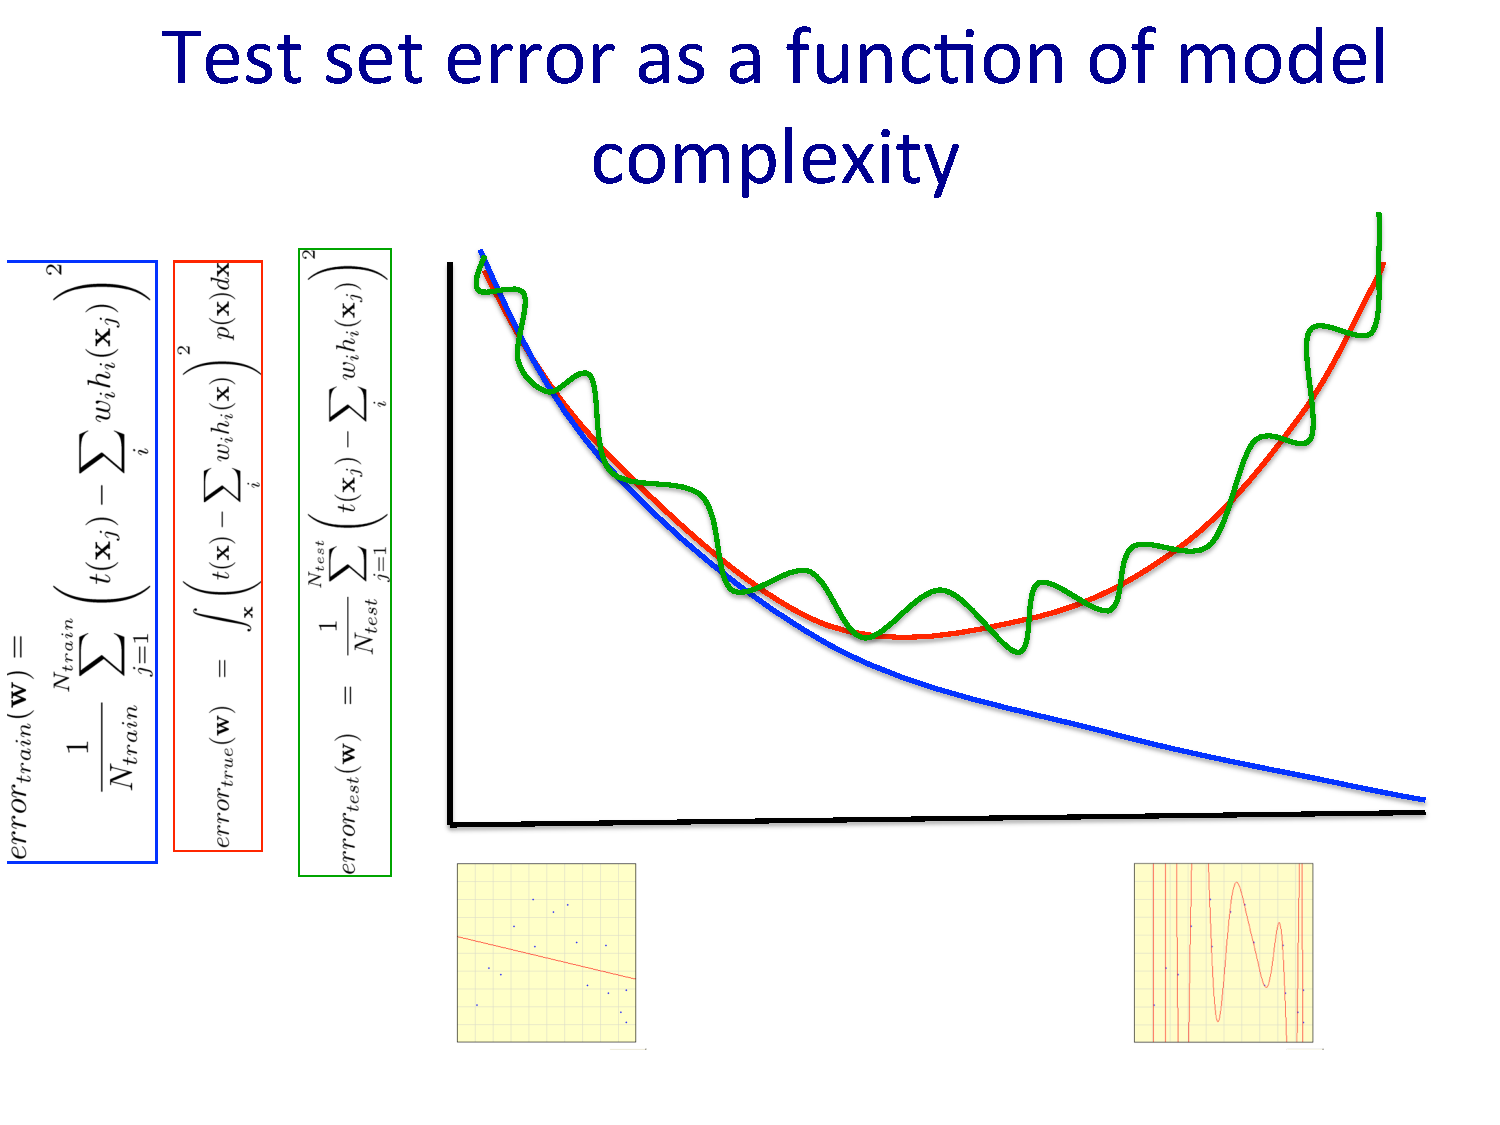
\includegraphics[width=3in]{figures/errors_as_f_of_complexity.pdf}   \hfill \\
(blue is train, red is true, green is test) \hfill \\

\subsubsection{overfitting}
Assume: \hfill \\
* Data generated from distribution D(X,Y). \hfill \\
* A hypothesis space H \hfill \\
Define:  \hfill \\
* Training error: $error_{train}(h)$ \hfill \\
* Data (true) error: $error_{true}(h)$ \hfill \\
We say $h$ \textbf{overfits} the training data if there exists an $h' \in H$ such that:  \hfill \\ 
* $error_{train}(h) < error_{train}(h)'$ and $error_{true}(h) > error_{true}(h)'$

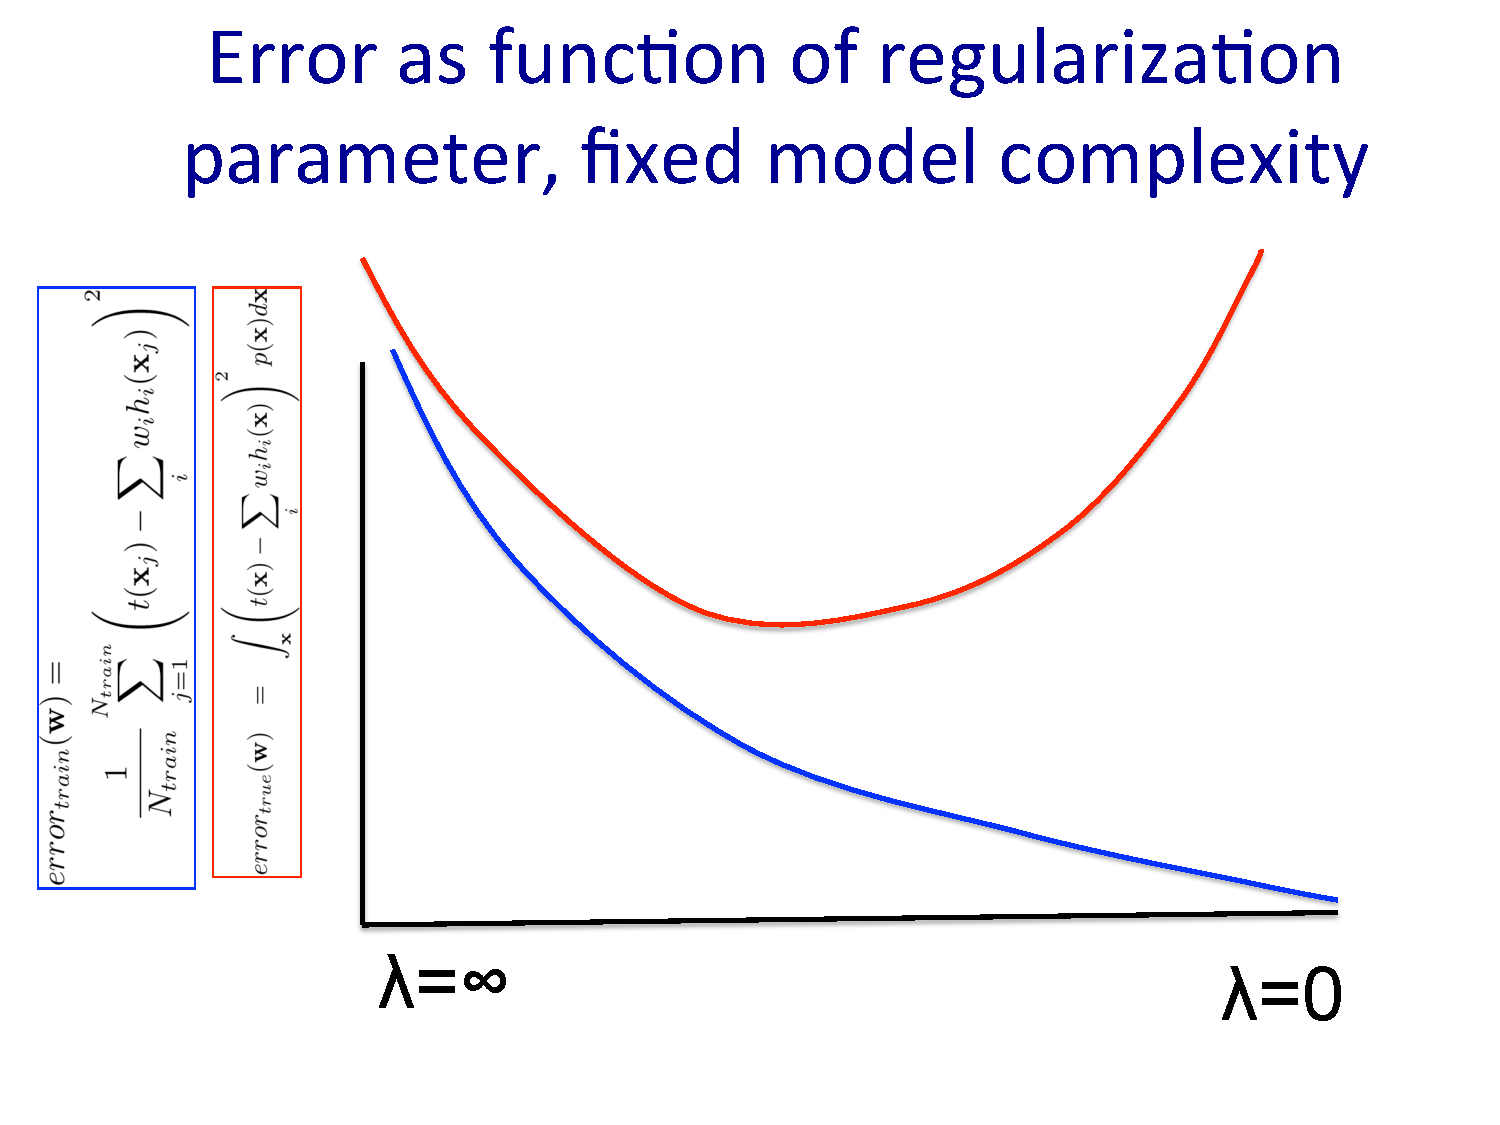
\includegraphics[width=2in]{figures/Error--vs_lambda--fixed_model_complexity.pdf}   \hfill \\
Lambda (the regularization parameter) is fixed.  Blue = training set error.  
Leads to overfitting/too-large-parameters when $\lambda$ --> 0. 
Red = true error, which likes a happy medium $\lambda$.  \hfill \\  \hfill \\

\textbf{Warning}: your test set is only unbiased if you never ever ever do \textbf{any} learning on the data. 
This includes using the test data to select for the degree of the polynomial you fit.   \hfill \\  \hfill \\
(Recall, you can create a held-out/validation set from your training data or do k-fold validation.)  \hfill \\
\hfill \\

The height of the true error (red curve) is the "bias".  \hfill \\

\subsubsection{What you need to know}
Regression:
\begin{itemize}
	\item Basis functions = features
	\item Optimizing a sum of squared errors
	\item Relationship between regression and Gaussians
\end{itemize}
Regularization
\begin{itemize}
	\item Ridge regression math
	\item LASSO formulation
	\item How to set lambda
\end{itemize}
Bias-Variance trade-off







\section{Naive Bayes}
\smallskip \hrule height 2pt \smallskip
Parameters are from data statistics; probabilistic interpretation.  \hfill \\ % lec 7 end
Train on Y conditioned on x. \hfill \\  % Friday wk 4 audio transcription.
Bayes: $P(Y=X) \propto P(X|Y)P(Y)$.  
But that is ($2^N$) parameters, and you might not be able to make a model with that many ($N$) parameters if your training data has a lot of features.
So you can add some assumptions that take you from $2^N$ parameters down to $2N$ of them. \hfill \\  % Friday wk 4 audio transcription.

Study the problem feature by feature.  Assume chunks of features are conditionally independent.  This is a false assumption, but often works.  
(Features are probably not independent, but it turns out to be reasonably safe to assume so.)
MAP is the foundation for Naive Bayes classifiers.  % http://www.cs.cmu.edu/~tom/10601_sp08/slides/recitation-mle-nb.pdf
 \hfill \\
  \hfill \\
Do we do optimization with NB?  
No.  We start with the joint distribution: $P(x|y)*prior$, $\dots$, take the max.  % week 6 audio
    Not ML optimizing.  Not required to optimize every time we learn something. % week 6 audio

Vocabulary
\begin{itemize}
	\item \textbf{$h_{NB}(x)$} the function that returns the best class.  %Erick 2/4/2016
	\item Loss function:
	in Naive Bayes the loss function is the negative log likelihood of the data given the parameters: $- \ln(P(X, y | w))$.  % TA e-mail 3/15/2016
\end{itemize}

Advantages:
\begin{itemize}
	\item Fast to train (single scan/pass through data). Fast to classify  % http://www.cs.ucr.edu/~eamonn/CE/Bayesian%20Classification%20withInsect_examples.pdf
	\item Not sensitive to irrelevant features  % http://www.cs.ucr.edu/~eamonn/CE/Bayesian%20Classification%20withInsect_examples.pdf
	\item Handles real and discrete data   % http://www.cs.ucr.edu/~eamonn/CE/Bayesian%20Classification%20withInsect_examples.pdf
	\item Handles streaming data well   % http://www.cs.ucr.edu/~eamonn/CE/Bayesian%20Classification%20withInsect_examples.pdf
	\item conditional independence assumption $\rightarrow$ we don't need to see occurrences of joint assignments to estimate their probabilities.  % HW 2 forum
\end{itemize}
Disadvantages:
\begin{itemize}
	\item Assumes independence of features  % http://www.cs.ucr.edu/~eamonn/CE/Bayesian%20Classification%20withInsect_examples.pdf
	\item All observations have equal weight in prediction. % http://www.cs.ucr.edu/~eamonn/CE/Bayesian%20Classification%20withInsect_examples.pdf
\end{itemize}

Vocab:
\begin{itemize}
	\item \textbf{prior}:  $P(Y)$, the probability of a label/class.
	\item \textbf{Likelihood}: $P(\bm{X} | Y)$. 
	%\item 
	%\item \textbf{}
\end{itemize}
 
\subsubsection{Conditional independence}
$X$ is conditionally independent of $Y$ given $Z$ if the probability distribution
for $X$ is independent of the value of $Y$, given the value of $Z$: \hfill \\
$(\forall i, j, k)$ $P(X=i | Y = j | Z=k) = P(X=i | Z=k)$.  \hfill \\
E.g. P( Thunder $|$ Rain, Lightening) = P(Thunder $|$ Lightning) \hfill \\
Equivalent to P(X, Y $|$ Z) = P(X $|$ Z) P(Y $|$ Z)  \hfill \\ \hfill \\

TODO: put in plain english. 

HW 2 forum: \hfill 
Naive Bayes assumption (is): \hfill \\
$P(D1, D2|H) = P(D1|H)P(D2|H)$, everything else follows from the rules of probability.


\subsubsection{Naive Bayes Assumption}
Features are independent given the class: \hfill \\
\begin{align*}
	P(X_1, X_2 | Y) &= P(X_1 | X_2, Y) P(X_2 | Y)  \\
				&= P(X_1 | Y) P(X_2| Y)      \\
				& \mbox{more generally:}      \\
	P(X_1, \dots, X_n | Y) &=  \prod_i P(X_i | Y)			
\end{align*}

This reduces the number of parameters a lot!
Say you had 5 features.  
Before this assumption, each of your 5 features could be dependent.   Then you have to assign a probability to each state.  If each is binary, then you can say $2^5$.  
After this assumption, you would just have 5 parameters.   \hfill\\ \hfill \\

\subsubsection{Homework clarifications}
\underline{Homework 2 TA notes:}  \hfill \\
Naive Bayes gives us a way to compute the whole joint distribution P(Cold, Headache, Cough, SoreThroat). Once we have this, everything else follows from the sum/chain rules of probability:

From the definition of conditional probability (which is the chain rule in disguise):
P(Cold | notHeadache, Cough, SoreThroat) = P(Cold, not Headache, Cough, SoreThroat)/P(not Headache, Cough, Sore Throat)

From the sum rule we see that the denominator is:
P(not Headache, Cough, SoreThroat) = P(Cold, not Headache, Cough, SoreThroat) + P(not Cold, not Headache, Cough, SoreThroat)

Thus the entire conditional probability can be computed using the joint distribution (which can be computed from the factorization and the estimates from the dataset).

The reason we want to include the denominator is to make sure that P(not Headache, Cough, SoreThroat) is non-zero (as asked in another post). It's not zero here, but if it was that would mean we can't really ask about the prediction P(Cold | not Headache, Cough, SoreThroat), since this is only defined when P(not Headache, Cough, SoreThroat) is non-zero. In practice people just assume this isn't an issue, and directly maximize the joint probability.

\hfill \\
The point of Naive Bayes isn't that $P(H| D1, D2)$ is proportional to $P(H, D1, D2)$, as this is true for any distribution (Here Di are the data, H is the hypothesis for some arbitrary problem). The point is that we assume the conditional independence $P(D1, D2| H)$ is $P(D1|H) P(D2|H)$. No the denominator is not used in practice, but that's a simplifying assumption that only works if none of your conditional probabilities are zero (which in turn means all joint probabilities are nonzero). Using the denominator doesn't defeat the point of Naive Bayes, it just ensures that $P(Cold | not Headache, Cough, SoreThroat)$ is well defined as explained above. \hfill \\

You should be using the conditional independence assumption from Naive Bayes to compute the joint probabilities in the numerator/denominator: e.g. $P(H, D1, D2) = P(H)*P(D1|H)*P(D2|H)$, where $P(H)$, $P(D1|H)$, $P(D2|H)$ are estimated from the data (with or without Laplacian smoothing). The conditional independence assumption means that we don't estimate $P(D1 = True, D2 = False | H)$ from the number of times we see $(D1= True, D2=False)$ together, we split $P(D1=True, D2=False|H)$ into $P(D1=True|H)*P(D2=False|H)$ and estimate each conditional independently. This is a huge simplification, since if we have N binary variables, we would need to see $2^N$ combinations to see all of the joint assignments (D1,...DN).
\hfill \\ \hfill \\

[Cold] is not independent of [Headache], [Cough], or [SoreThroat]. Consider: if [Cold] were in fact not related to these variables, we wouldn't be predicting [Cold] from them. Furthermore, [Cough] and [Headache] are not independent, since both are not independent of [Cold]. However, the Naive Bayes assumption is that once you account for that dependence, [Cough] and [Headache] are independent.

Here's a common-sense description of this. If you go around talking to people, you notice that some have headaches, and some have colds. At first, you are confused and wonder why this might be. Is it, perhaps, that coughing all the time is so annoying that it eventually causes people headaches? But then you realize that there is a common illness, the cold, that causes both headaches and coughs. Aha! you say. So you start asking people not only if they have a headache and a cough, but also whether or not they have a cold. You find that among people with colds, having a headache and having a cough seem like unrelated phenomena. And among people without colds, headaches and colds are again unrelated. This is the world that Naive Bayes assumes.

You ask "Would it be the case then that P(Cd, H, C, S) = P(H, C, S | Cd) P(Cd) ?" Yes. That fact is the definition of conditional probability, and it is a basic fact of probabilities. It is true for all variables, in all situations, no matter what assumptions you make. It is true whether Cd and H are independent or not, whether they represent colds or aliens or whatever. You can always use this fact about any variables. \hfill \\
-------------

Naive Bayes is not about ignoring the denominator. This seems to have been a common misunderstanding.

Naive Bayes is an independence assumption; namely, that your input features are independent given the output feature.

This assumption allows you to estimate probabilities like P(X, Y, Z) in terms of other probabilities P(X, Y) and P(X, Z). Since it relates probabilities to each other, it makes it easier to estimate probabilities from samples. For example, if you are trying to detect if a message is spam, you want to compute P(spam | Hello, I, am, Prince, Albert, of, Nigeria, ...), and you may have never seen any points with text (Hello, I, am, Prince, Albert, of, Nigeria, ...) and so would not have any estimate of the probability that that message is spam. With Naive Bayes, you would rewrite this to in terms of the probabilities P(spam | Hello) and P(spam | I) and P(spam | am) and ..., all of which you can compute because you have seen many messages with the words "Hello", or "Prince", or "Nigeria", and know the associated probabilities of spam.

This question asks you to use the Naive Bayes assumption to estimate a probability value given some data, which is exactly what you use Naive Bayes for.

\subsubsection{Naive Bayes Classifier}
Given:
\begin{itemize}
	\item a prior $P(Y)$  
	\item $n$ conditionally independent features $\bm{X}$ given the class $Y$
	\item calculated likelihood for each $X_i$ of the form $P(X_i | Y)$
\end{itemize}
Your decision rule is:   (note $h_{NB}$ is Naive Bayes, not Neg Binom) 
\begin{align*}
	y^* = h_{NB}(x) &= \argmax_y P(y) P(x_1, \dots, x_n | y)   \\
			&=  \argmax_y P(y) \prod_i P(x_i | y)
\end{align*}

\noindent
Although the assumption that the predictor (independent) variables are independent is not always accurate, it does simplify the classification task dramatically, since it allows the class conditional densities $p(x_k | C_j)$ to be calculated separately for each variable, i.e., it reduces a multidimensional task to a number of one-dimensional ones.
In effect, Naive Bayes reduces a high-dimensional density estimation task to a one-dimensional kernel density estimation. Furthermore, the assumption does not seem to greatly affect the posterior probabilities, especially in regions near decision boundaries, thus, leaving the classification task unaffected.
% http://www.statsoft.com/textbook/naive-bayes-classifier

Na�ve Bayes is NOT sensitive to irrelevant features.  % http://www.cs.ucr.edu/~eamonn/CE/Bayesian%20Classification%20withInsect_examples.pdf
However, this assumes that we have good enough estimates of the probabilities, so the more data the better.

\subsubsection{Digit classification example}
Simplify images of digits to pixels, and assign them True or False for whether they are "on".  \hfill \\
Each input maps to a feature in a vector.  E.g. pixel in the 0th for and 0th column is $F_{0,0}$.   \hfill \\
The Naive Bayes model is: \hfill \\
$ \displaystyle P(Y | F_{0,0}, \dots , F_{15,15}) \propto P(Y) \prod_{i,j} P(F_{i,j} | Y)$.
We assume the features are independent given the class.  
We need to learn the distribution of pixels on at each pixel given each number.  \hfill \\
How to calculate the prior, P(Y): \hfill \\
$\displaystyle P(Y) = \frac{count(Y=y)}{\sum_{y'} Count(Y=y'}$ (denominator is summing over all y values) \hfill \\
How to calculate the likelihood:  \hfill \\
$\displaystyle P(X_i =x | Y=y) = \frac{Count(X_i=x, Y=y)}{\sum_{x'}Count(X_i=x', Y=y)}$


\subsubsection{For binary features, use the Beta prior and MAP.} 
Just like likeihood of binomial previously! 
$\displaystyle P(\theta | D) = \frac{\theta^{\beta_H + \alpha_H - 1}(1-theta)^{\beta_T + \alpha_T - 1}}{B(\beta_H + \alpha_H, \beta_T + \alpha_T)} \approx Beta(\beta_H + \alpha_H, \beta_T + \alpha_T) $
Chose $\theta$ using MAP:  \hfill \\
$\displaystyle  \widehat{\theta} = \argmax_\theta P(\theta | D) = \frac{\alpha_H + \beta_H - 1}{\alpha_H + \beta_H + \alpha_T + \beta_T - 2}$.  \hfill \\
Once again, the Beta prior is equivalent to adding extra observations for each feature. \hfill \\
If you don't have a lot of observations, the prior is important.  \hfill \\
And as the number of observations goes to $\infty$, the prior is "forgotten". 

\subsubsection{Multinomials: Laplace Smoothing}
\underline{Laplace's estimate}: \hfill \\
Pretend you saw every outcome $k$ extra times: \hfill \\
$\displaystyle P_{LAP, k}(x) = \frac{c(x) + k}{N + k|X|}$ \hfill \\
$N = $ number of observations.  \hfill \\
$|X| = $ the number of categories you are counting.  \hfill \\
$k$ is the strength of the prior; how much of the prior information you are going to enforce\hfill \\  \hfill \\

Example: 
$\displaystyle P_{LAP, 0}(X) = \langle \frac{2}{3}, \frac{1}{3} \rangle$.  \hfill \\
Set $k=1$.  $|X|$ is 2.  $N$ is 3.  
$\displaystyle P_{LAP, 1}(X) = \langle \frac{3}{5}, \frac{2}{5} \rangle$  \hfill \\
$\displaystyle P_{LAP, 100}(X) = \langle \frac{102}{203}, \frac{101}{203} \rangle$  \hfill \\

\underline{Laplace for conditionals:}
Smooth each condition independently:  \hfill \\
$\displaystyle  P_{LAP, k}(x|y) = \frac{c(x,y) + k}{c(y) + k |X|}$

\subsubsection{Subtleties of the NB classifier}
\textbf{(1) Usually the features are not conditionally independent}: \hfill \\
$P(X_1, \dots, X_n | Y) \neq \prod_i P(X_i | Y)$ \hfill \\
The actual probabilities $P(Y | \bm{X})$ are often biased towards 0 or 1.  
Nonetheless, NB is the single most used classifier out there.  
It performs well even when the independence assumption is violated.  \hfill \\
\textbf{(2) Overfitting} \hfill \\
Conditional probabilities can easily be calculated as zero. 
Zero probabilities kill that class' chance at being called. \hfill \\
??? If the feature is binary, we can use MAP with a beta prior. 
??? That's equivalent to adding extra observations for each feature. 

\subsubsection{NB for text classification}
\begin{itemize}
	\item Need a feature vector with a suitably small number of features.
		Bag of words model is commonly used. 
	\item $i$ is the $i^{th}$ word
	\item NB assumption(\_\_\_) helps a lot.  
		$P(X_i=x_i |Y=y)$ is just the probability of observing word $x_i$ in a document on topic $y$.  
		$ \displaystyle  h_{NB}(x) = \argmax_y P(y) \prod_{i=1}^{LengthDoc} P(x_i | y)$  
	\item Additional assumption: bag of words model. \hfill \\
		Order of words ignored.  Works really well.  \hfill \\
		$P(X_i = x_i | Y=y) = P(X_k = x_i | Y=y)$  ($k$ is the $k^{th}$ word (?); all positions have the same distribution).  \hfill \\
		$P(y) = \prod_{i=1}^{LengthDoc} P(x_i | y)$
	\item Prior, $P(Y)$, is the fraction of documents of each topic.
	\item Likelihood, $P(X_i | Y)$ is count for how many times you saw the word in documents of this topic.  
		This distribution is shared across all positions $i$.
	\item Testing: Use Naive Bayes decision rule.  \hfill \\
		$ \displaystyle  h_{NB}(x) = \argmax_y P(y) \prod_{i=1}^{LengthDoc} P(x_i | y)$
\end{itemize}

\subsubsection{NB for continuous $X_i$}

\begin{itemize}
	\item $k$ is an index over all possible labels. 
	\item $i$ is the $i^{th}$ feature. Here it is the pixel.
	\item $j$ is the $j^{th}$ training example.  
	\item $X_i^j$ is the $i^{th}$ pixel in the $j^{th}$ training sample. 
	\item $Y^j$ is the label corresponding to the $j^{th}$ training example. 
	\item $y_k$ is the $k^{th}$ label
	\item $j$ is $j^{th}$ training example.  
	\item $\delta(x) = 1$ if x true, else 0. 
	\item $h$: the function that returns the best class.  % Erick 2/4/2016
\end{itemize}


Example: character recognition where the darkness of each pixel is continuous.  \hfill \\
\subsection{Gausian Naive Bayes (GNB) for continuous features}

Find parameter that makes all the data points most likely.
What parameters explain our data best?  \hfill \\
 \hfill \\


Naive Bayes continuous video:  \url{https://www.youtube.com/watch?v=r1in0YNetG8}

	$ \displaystyle P(X_i = x | Y = y_k) = \frac{1}{\sigma_{ik} \sqrt{2 \pi}} e^\frac{-(x- \mu_{ik})^2}{2 \sigma_{ik}^2}$  \hfill \\
\begin{itemize}
	\item $\mu_{ik}$ is the mean of the values for the $i^{th}$ feature for the $k^{th}$ class. \hfill \\
	\item $\sigma_{ik}$ is the standard deviation of the values for the $i^{th}$ feature for the $k^{th}$ class. 
\end{itemize}	
	
Sometimes we assume one or both of these:
\begin{itemize}
	\item variance is independent of $Y$ (i.e. $\sigma_i$)
	\item variance is independent of $X_i$ (i.e. $\sigma_k$)
\end{itemize}
If we assume both, we assume just one $\sigma$ without subscripts. \hfill \\   \hfill \\

Estimating parameters for discrete $Y$ and continuous $X_i$:  \hfill \\
\begin{itemize}
	\item \textbf{mean}:  $\displaystyle \widehat{\mu}_{ik} = \frac{1}{\sum_j \delta(Y^j = y_k)} \sum_j X_i^j \delta(Y^j = y_k)$
		\begin{itemize}
			\item first term: divide by the number of training examples that are of class k. 
			\item second term: summing the continuous input of pixel i for all examples 
				in the training set that match label k.  
			\item so this is just an average brightness for pixel $i$ given class $k$ using 
				all the training data.   
		\end{itemize}
	\item \textbf{variance}:  $\displaystyle  \widehat{\sigma}_{ik}^2 = \frac{1}{\sum_j \delta(Y^j = y_k) - 1} \sum_j (x_i^j - \widehat{\mu}_{ik})^2 \delta(Y^j = y_k)$
		\begin{itemize}
			\item first term: divide by the number of training points of class k minus 1. 
			\item second term: sum the squared difference in brightness of pixel $i$ 
				compared to the mean for that pixel and label. 
		\end{itemize}
\end{itemize}
We don't need to use a Gaussian for the prior, $P(y)$.  We aren't optimizing over it, so it is safe to count.  % audio week 5 

\subsection{When Bayes Classifier is Optimal:}
In Bayes we are learning the function $h$ that produces labels $Y$ based on inputs $\bm{X}$.  
More formally: \hfill \\
$h : \bm{X} \mapsto Y$, or \hfill \\
we are learning "the function h that maps features $\bm{X}$ to labels Y". \hfill \\ \hfill \\

If you know the true $\displaystyle P(Y | \bm{X})$, then \hfill \\
$\displaystyle h_{Bayes} = \argmax_y P(Y=y | \bm{X} = x)$.   \hfill \\  \hfill \\
Note the subscript is Bayes, not Naive Bayes; no assumption of conditional independence.
Also, the conditionality is back to likelihood instead of posterior.  \hfill \\  \hfill \\

Theorem: Bayes (not NB) classifier $h_{Bayes}$ is optimal.  \hfill \\
$error_{true}(h_{Bayes}) \leq error_{true}(h)$, $\forall h$ \hfill \\
\hfill \\
\textit{This is theoretical result: we don't know $P(\bm{x})$.  We can't calculate the true Bayes classifier b/c we don't know the distribution of all the data.)}
We also don't know $P(Y | \bm{X})$, the true class' highest probability.  Usually that's hidden; if we knew it we would go home happy.  


Plain english: the predictions you get from Bayes are better than any other function/prediction available. \hfill \\ \hfill \\
Proof:  
\begin{align*}  % changed notation to capital p, X, Y
	P_h(error) = \int_x P_h & (error | \bm{X}) P(\bm{X}) \\  
		& \mbox{           def. of error: } P_h(error| \bm{x}) = \int_y \delta(h(\bm{X}), Y) P(Y| \bm{X}) \\
		& \mbox{               (note, usually we'd sum over the classes, Y)}  \\
			= \int_x \int_y & \delta(h(\bm{X}), Y) P(Y | \bm{X}) P(\bm{X})  \\
			& \mbox{     (the double integral is zero when $P(Y | \bm{X})$ is largest,} \\
			& \mbox{     which is when the correct classification was selected.)}
\end{align*} 
We are averaging over novel data sets that are generated under the same conditions.

%Note that this is different notation than the rest.  Large vs small P.  
Different notation: delta has a comma in the parentheses and not an equality.   \hfill \\
\begin{itemize}
	\item $P_h(error)$ is probability of error across all classifications. 
	\item $\delta(h(\bm{X}, Y)$ is 1 if your X is classified right and 0 if not. 
	\item $P_h(error| \bm{x})$ is the probability that your classification is wrong.  
	\item $\int_x P_h (error | \bm{X}) P(\bm{X}) $ is the expectation of the errors.  
	\item $\delta(h(\bm{X}), Y)$ is 
\end{itemize}

Proof in words:  ??? 

Aside: note that for one classification y is not a vector.  It is a point. 


\section{Logistic Regression}
\smallskip \hrule height 2pt \smallskip

Another probabilistic approach to classification (categorical predictions).  
 \hfill \\
Discriminative: learn $P(Y|X)$ directly then discriminate between classes.    % Week 5 audio. 
We solved similar problems using Bayes before (a generative approach).  
	But if we don't want to bother with modeling all those joint or conditional probabilities, we can do this discriminative approach instead. \hfill \\  %Wed 2/3 audio transcription.

Logistic Regression is the discriminative counterpart to a Naive Bayes generative classifier over Boolean features.  % https://www.cs.cmu.edu/~tom/mlbook/NBayesLogReg.pdf
The difference between logistic and Naive Bayes is just one word: "conditional".   % wk 5 audio
We are maximizing conditional log likelihood, that is conditional on X.  
	We are not going to spend our time encoding the distribution over X.   % wk 5 audio

\hfill \\   \hfill \\

Can use discrete or continuous outputs. \hfill \\ % https://www.youtube.com/watch?v=zAULhNrnuL4
It's a linear classifier; the decision rule is a hyperplane. \hfill \\  % Slide 6 summary
You optimize it (find weights) by gradient ascent, which works because it is concave.    \hfill \\  % Slide 6 summary
You can use "maximum conditional a posteriori" for regularization.    \hfill \\  % Slide 6 summary

\hfill \\ 

\underline{Summary from non-class sources:} \hfill \\
% https://www.youtube.com/watch?v=-Z2a_mzl9LM
We are still using linear regression in the inputs, but putting the result into a sigmoid function. \hfill \\
Recall $w_0 + w_1 x_1 + w_2 x_2 + w_3 x_3 = w^Tx$ and $x = (1, x_1, x_2, x_3)$.  \hfill \\
$P(death|x) = \sigma(w^Tx)$  %https://www.youtube.com/watch?v=-Z2a_mzl9LM
where $\sigma$, the sigmoid function,  converts your regression output into a sigmoid curve. \hfill \\
$\displaystyle \sigma(a) = \frac{1}{1+ e^{-a}} = \frac{1}{1+ e^{-(w_0 + w_1 x_1 + w_2 x_2 + w_3 x_3)}} = \frac{1}{1+ e^{-(w^Tx)}}$   \hfill \\ % https://www.youtube.com/watch?v=-Z2a_mzl9LM
\hfill \\

% https://www.youtube.com/watch?v=_Po-xZJflPM  :
We can convert this to a linear relationship by "taking the logit". \hfill \\
The logit (log odds) is the inverse of the logistic.  \hfill \\ %  https://en.wikipedia.org/wiki/Logistic_regression
$F(x) = \sigma(a)$ above.  It is the probability that the dependent variable equals a case, given some linear combination of the predictors.  It can range from $- \infty$ to $\infty$   % https://en.wikipedia.org/wiki/Logistic_regression
The logit is $\ln \frac{F(x)}{1-F(x)}$, or equivalently, after exponentiating both sides: \hfill \\
$\frac{F(x)}{1-F(x)} = e^{w^Tx}$  \hfill \\
The logit (i.e., log-odds or natural logarithm of the odds) is equivalent to the linear regression expression.

 


Note used odds ratio: $\frac{p}{1-p}$  \hfill \\
$\logit(\frac{1}{1+ e^{-(w^Tx)}}) = \log(\frac{\frac{1}{1+ e^{-(w^Tx)}}}{1-\frac{1}{1+ e^{-(w^Tx)}}}) $  \hfill \\ % https://www.youtube.com/watch?v=_Po-xZJflPM
We can now proceed with linear regression.  \hfill \\
Note that our predictions are now on the log scale; this impacts interpretation of the coefficients.  \hfill \\  %https://www.youtube.com/watch?v=_Po-xZJflPM 

\hfill \\ \hfill \\   

\underline{Lecture's presentation:} \hfill \\

Notation:  \hfill \\
\begin{itemize}
	\item $x_i^j$: the $i^{th}$ attribute of data point $j$
	\item $y^j$: the $j^{th}$ class  %(?)
	\item $x^j$: the $j^{th}$ training example
\end{itemize}

Once again we don't want to try to estimate $P(X,Y)$; that is challenging due to the size of the distribution. \hfill \\
We could make the Naive Bayes assumption and only need to calculate $P(X_i | Y)$, 
but if we want $P(Y|X)$, why not learn that directly?  You can use logistic regression. 
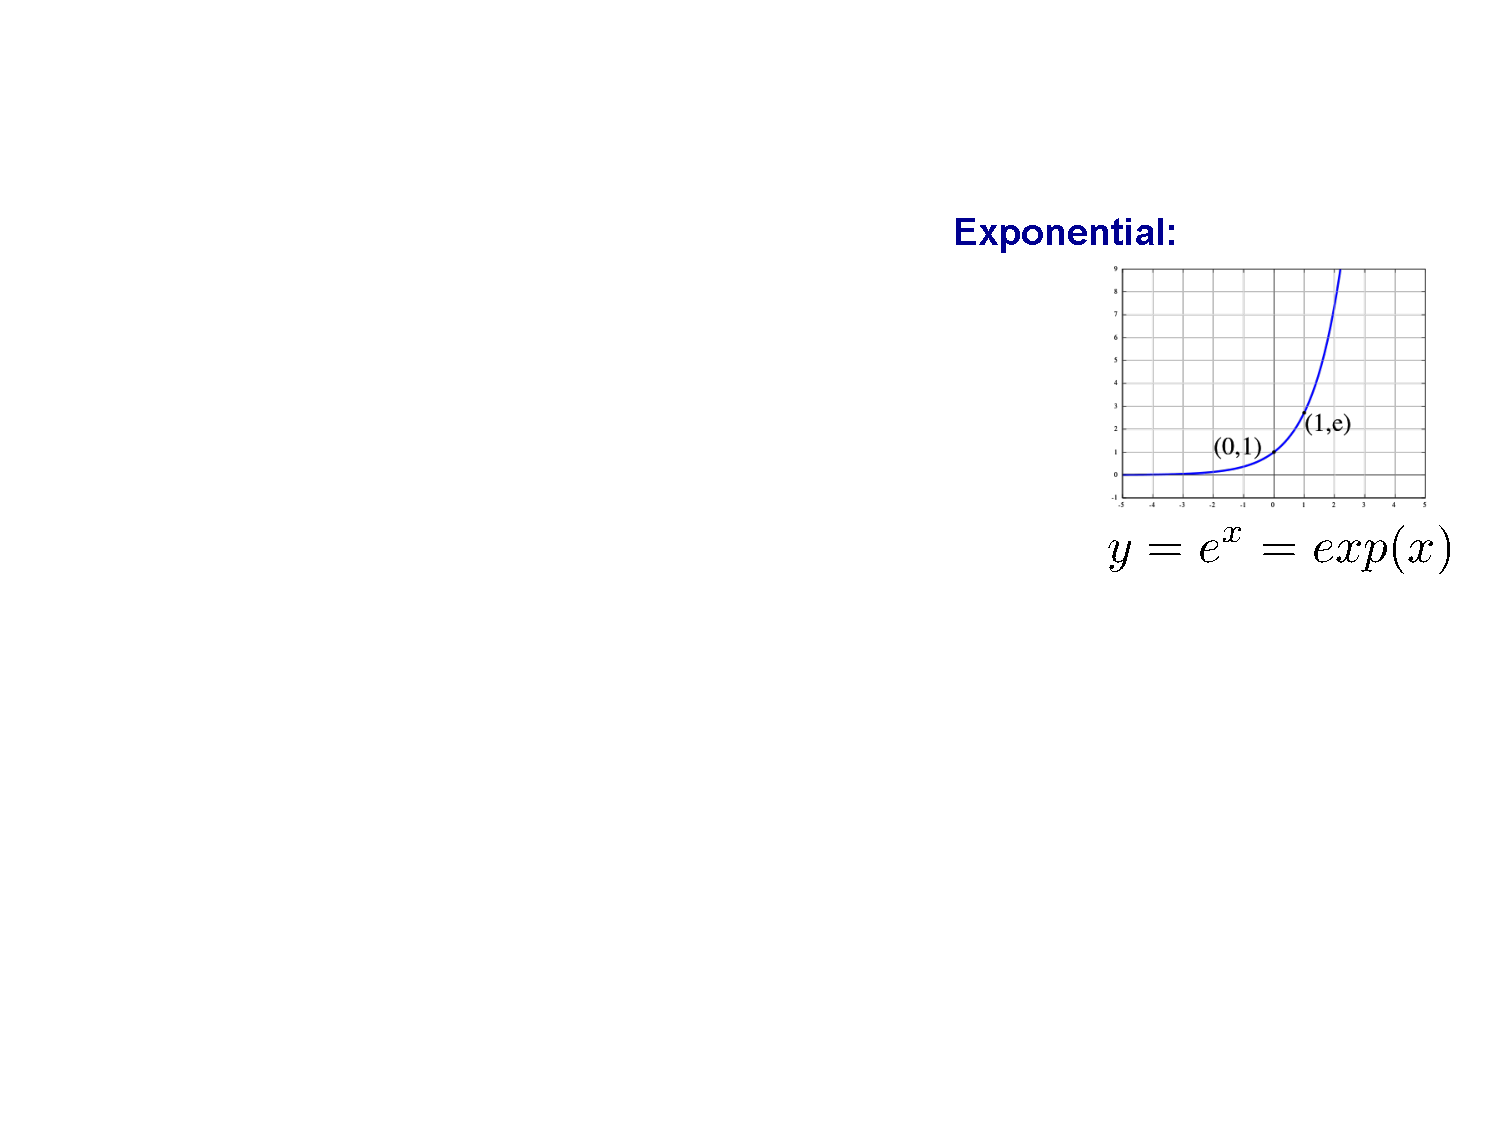
\includegraphics[width=1.5in]{figures/expo.pdf}     \hfill \\
\hfill \\

Reuse ideas from regression, but let the y-intercept define the probability.  \hfill \\
$P(Y=1|\bm{X, w}) \propto exp(w_0 + \sum_i w_i X_i)$  \hfill \\
With normalization constants:  \hfill \\
$\displaystyle  P(Y=0|\bm{X, w}) \frac{1}{1+ exp(w_0 + \sum_i w_i X_i)} $ \hfill \\
$\displaystyle  P(Y=1|\bm{X, w}) \frac{exp(w_0 + \sum_i w_i X_i)}{1+ exp(w_0 + \sum_i w_i X_i)} $ \hfill \\
Logistic function: 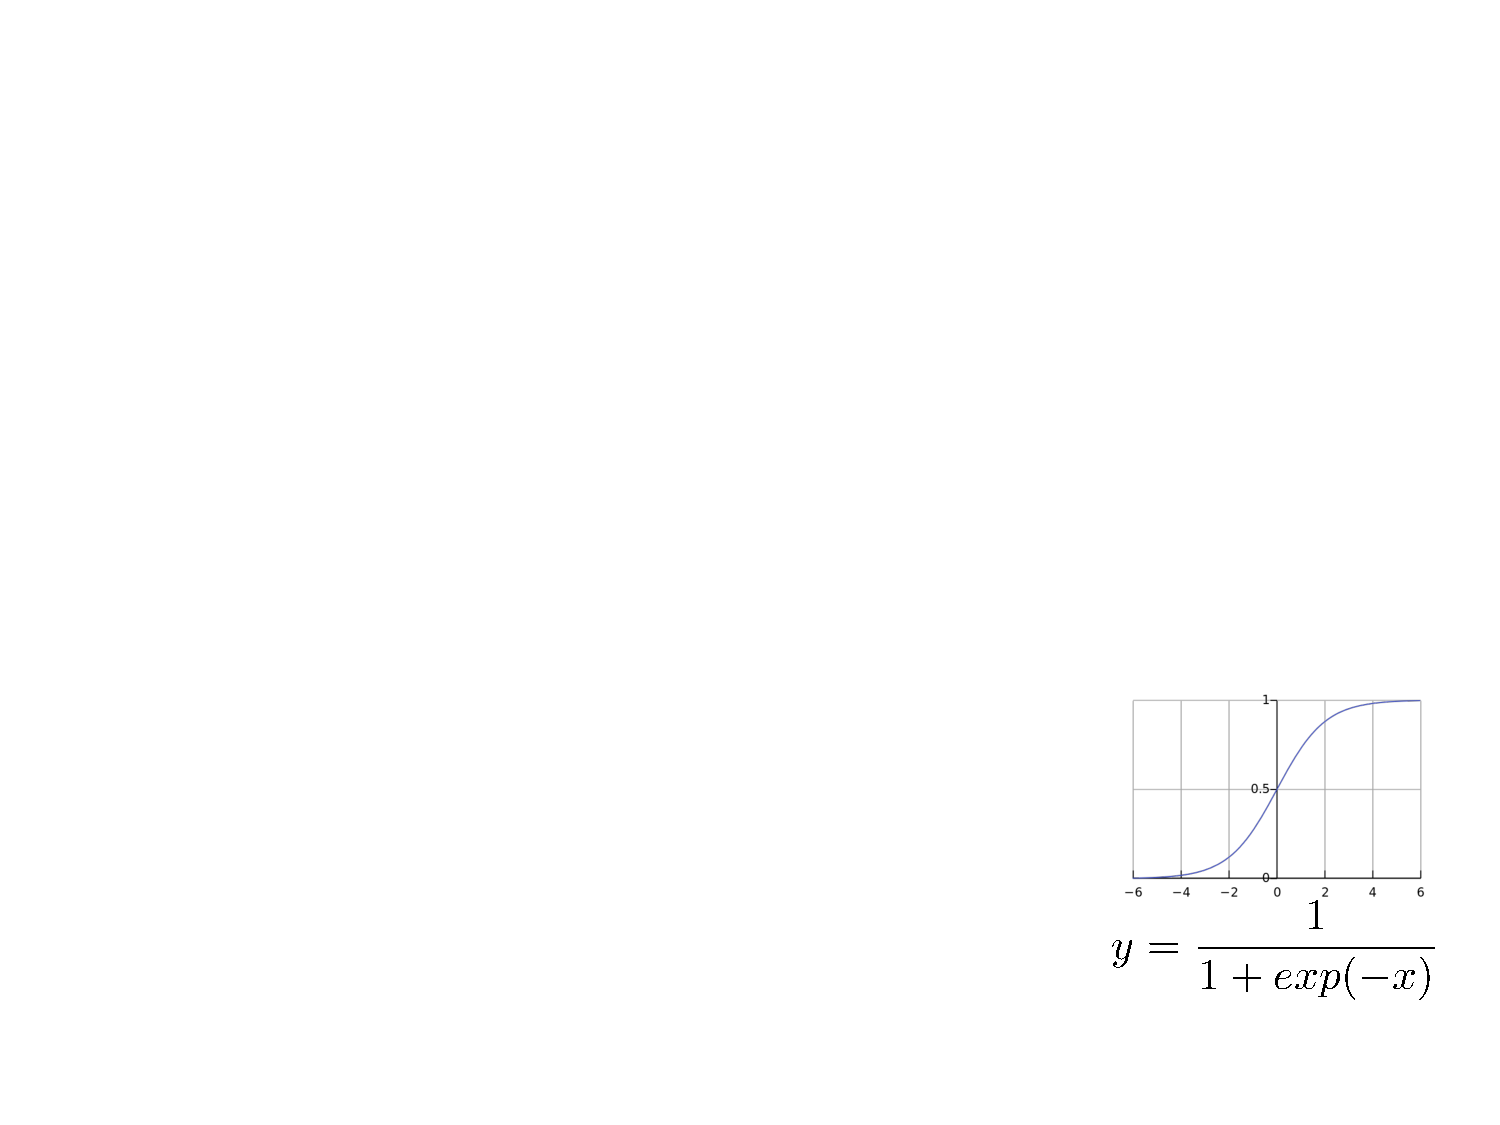
\includegraphics[width=1in]{figures/logistic.pdf}     \hfill \\
 \hfill \\
 
Making a decision boundary out of logistic equations:  \hfill \\
Output the $Y$ with the highest $P(Y|X)$.   \hfill \\
If binary Y, output Y=1 if $\displaystyle 1 < \frac{P(Y=1|X)}{P(Y=0|X)}$  \hfill \\
That simplifies to just $1 <exp(w_0 + \sum_i w_i X_i)$ or \hfill \\
$0 <w_0 + \sum_i w_i X_i$   \hfill \\
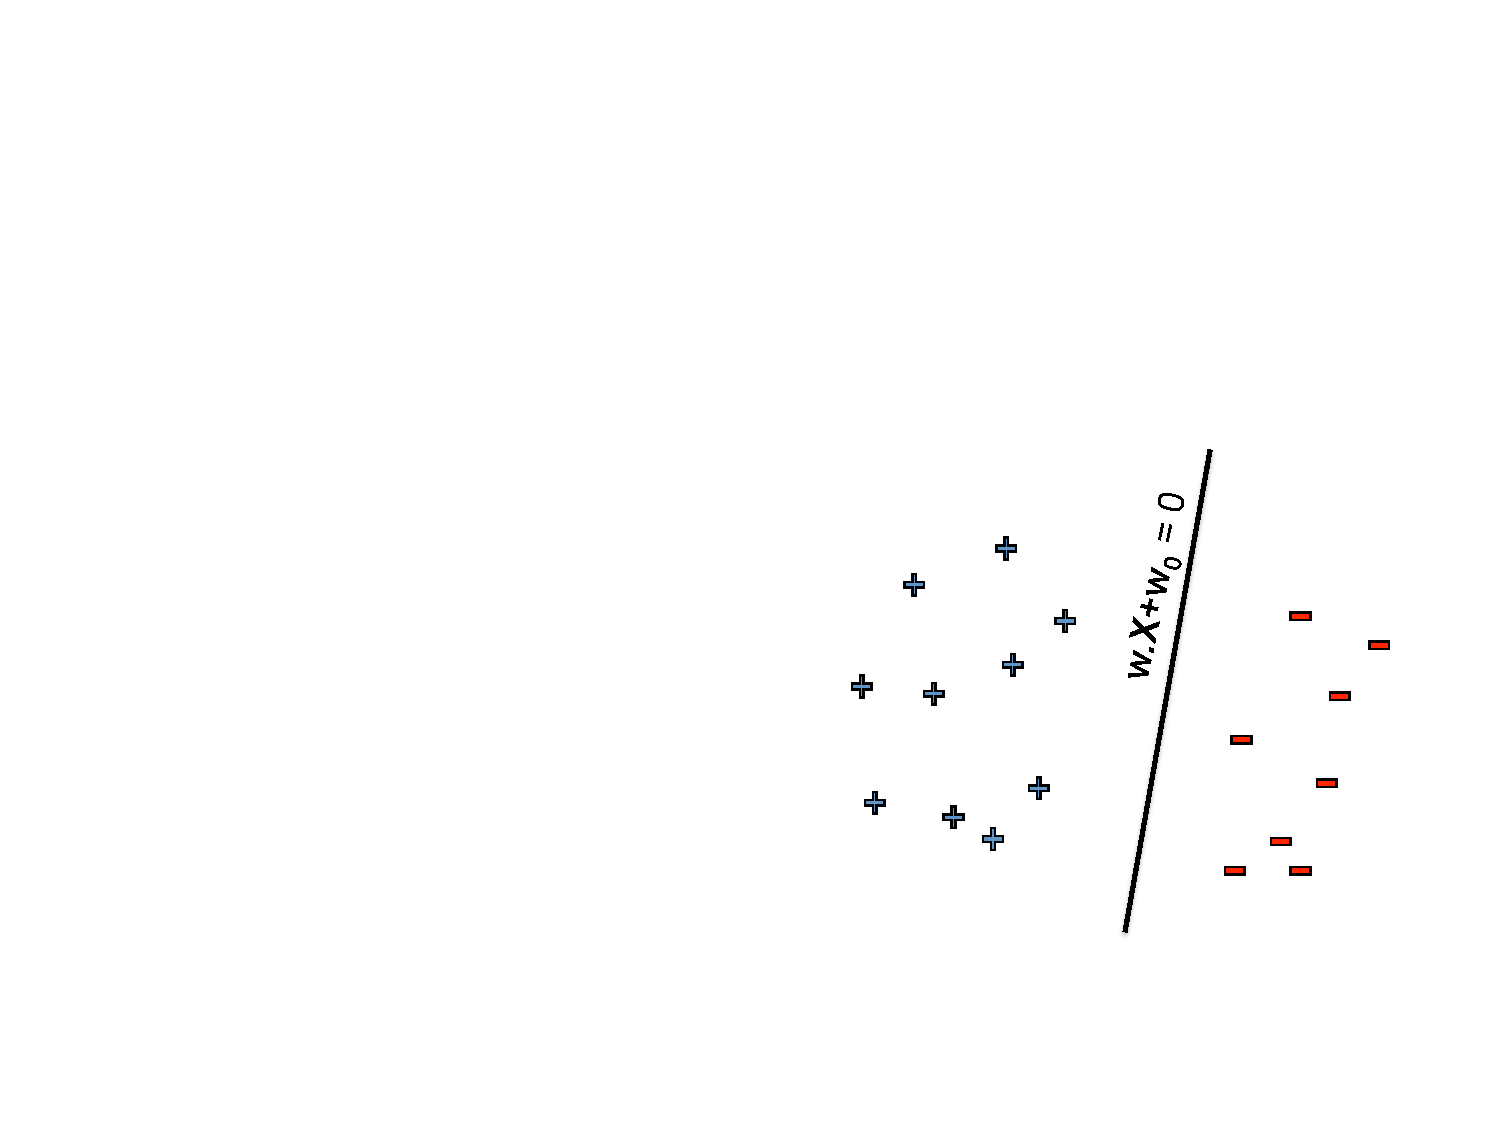
\includegraphics[width=.8in]{figures/logistic_boundary_linear.pdf}     \hfill \\
\textbf{The decision boundary is a line (or hyperplane), hence we have a linear classifier!} \hfill \\  \hfill \\

For $ \displaystyle P(Y=0 | \bm{X,w}) = \frac{1}{1 + exp(w_o + w_1 x_1)}$:  \hfill \\
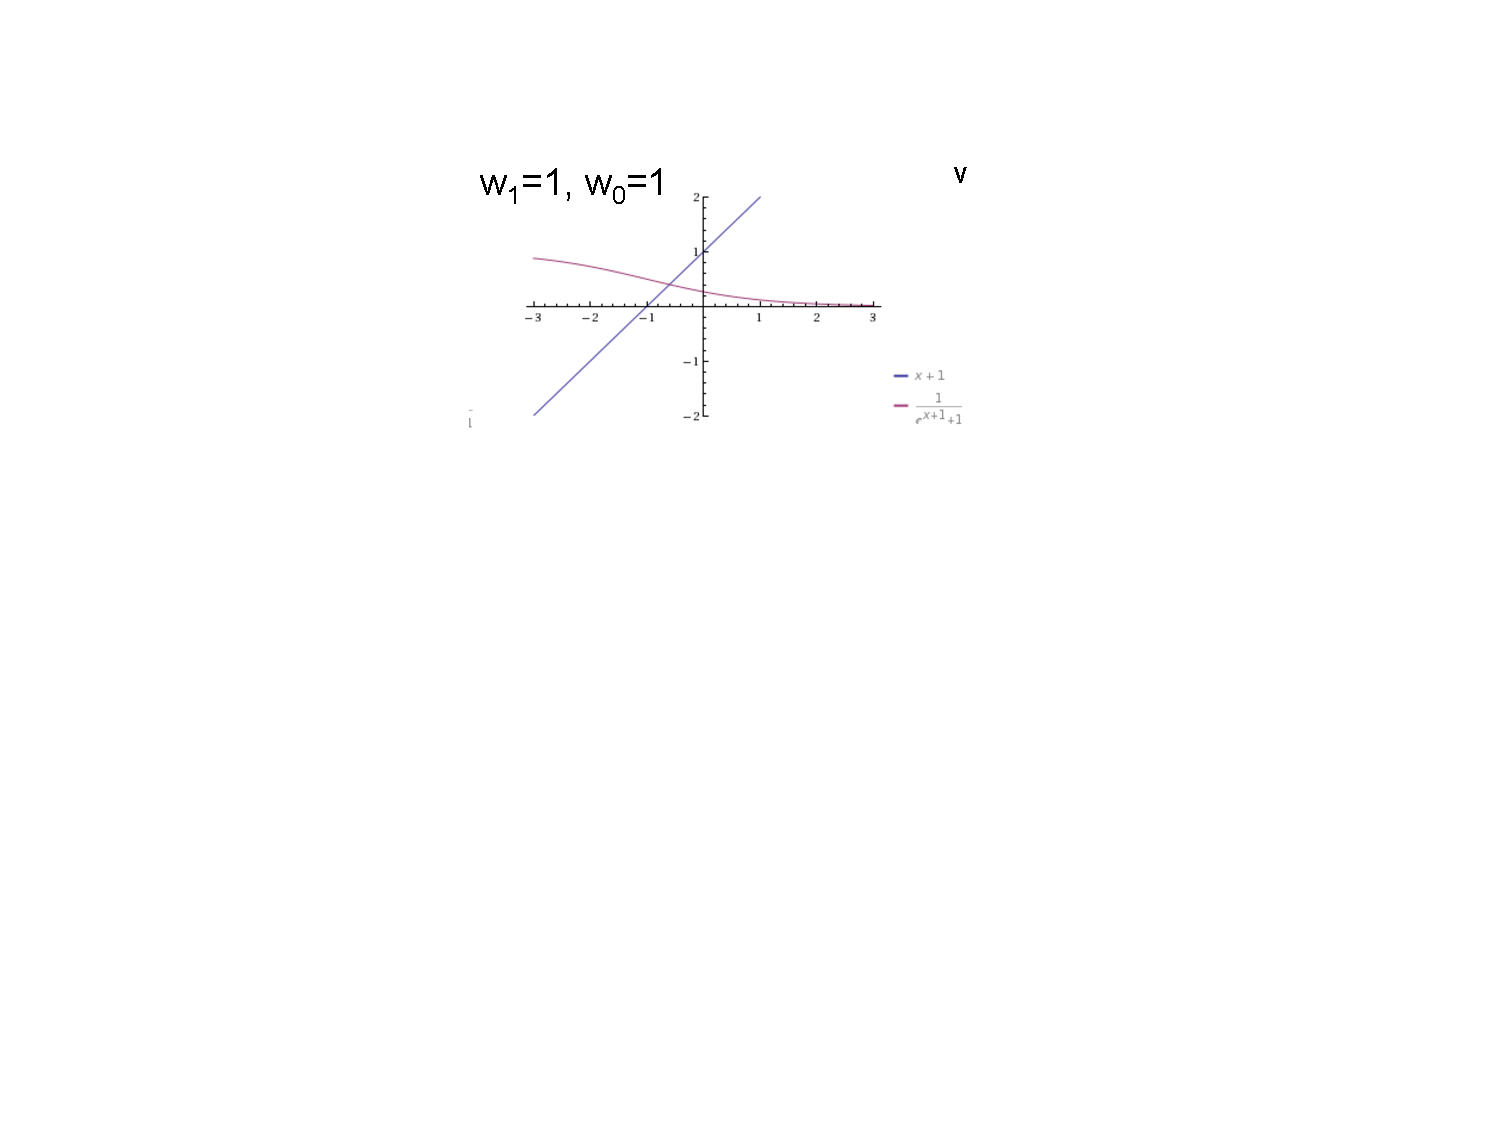
\includegraphics[width=2in]{figures/decision_boundary_example.pdf}   \hfill \\
(See notes for more $w_0, w_1$ values plotted.)  \hfill \\
In these plots, Y is the probability that the class is 1.    \hfill \\
The red curve is the sigmoid.  The blue line is the decision boundary.  \hfill \\
The decision boundary is from the equation $0 = w_1X + w_0$.  \hfill \\
% Erick advice: ignore the blue lines entirely.  don't need them to find probability distribution. 

\hfill \\
Larger weights result in a sharper curve.  The bias $w_0$ shifts there the middle of the curve is.   \hfill \\
The red sigmoid defines a probability distribution over $Y$ in \{0,1\} for every possible input X. \hfill \\
\hfill \\
The decision boundary leads to $P(Y=0|X, w) = 0.5$ when you are at the $y=0$ point on the line.   \hfill \\
(E/J words:  when the blue line crosses the x axis, that's when the sigmoid curve is above 1/2, which corresponds to classifying it as a no/0.)  \hfill \\
The slope of the line defines how quickly the probabilities go to 0 or 1 around the decision boundary. 
\hfill \\

2D inputs: \hfill \\
For $ \displaystyle P(Y=0 | \bm{X,w}) = \frac{1}{1 + exp(w_o + w_1 x_1 + w_2 x_2)}$:  \hfill \\
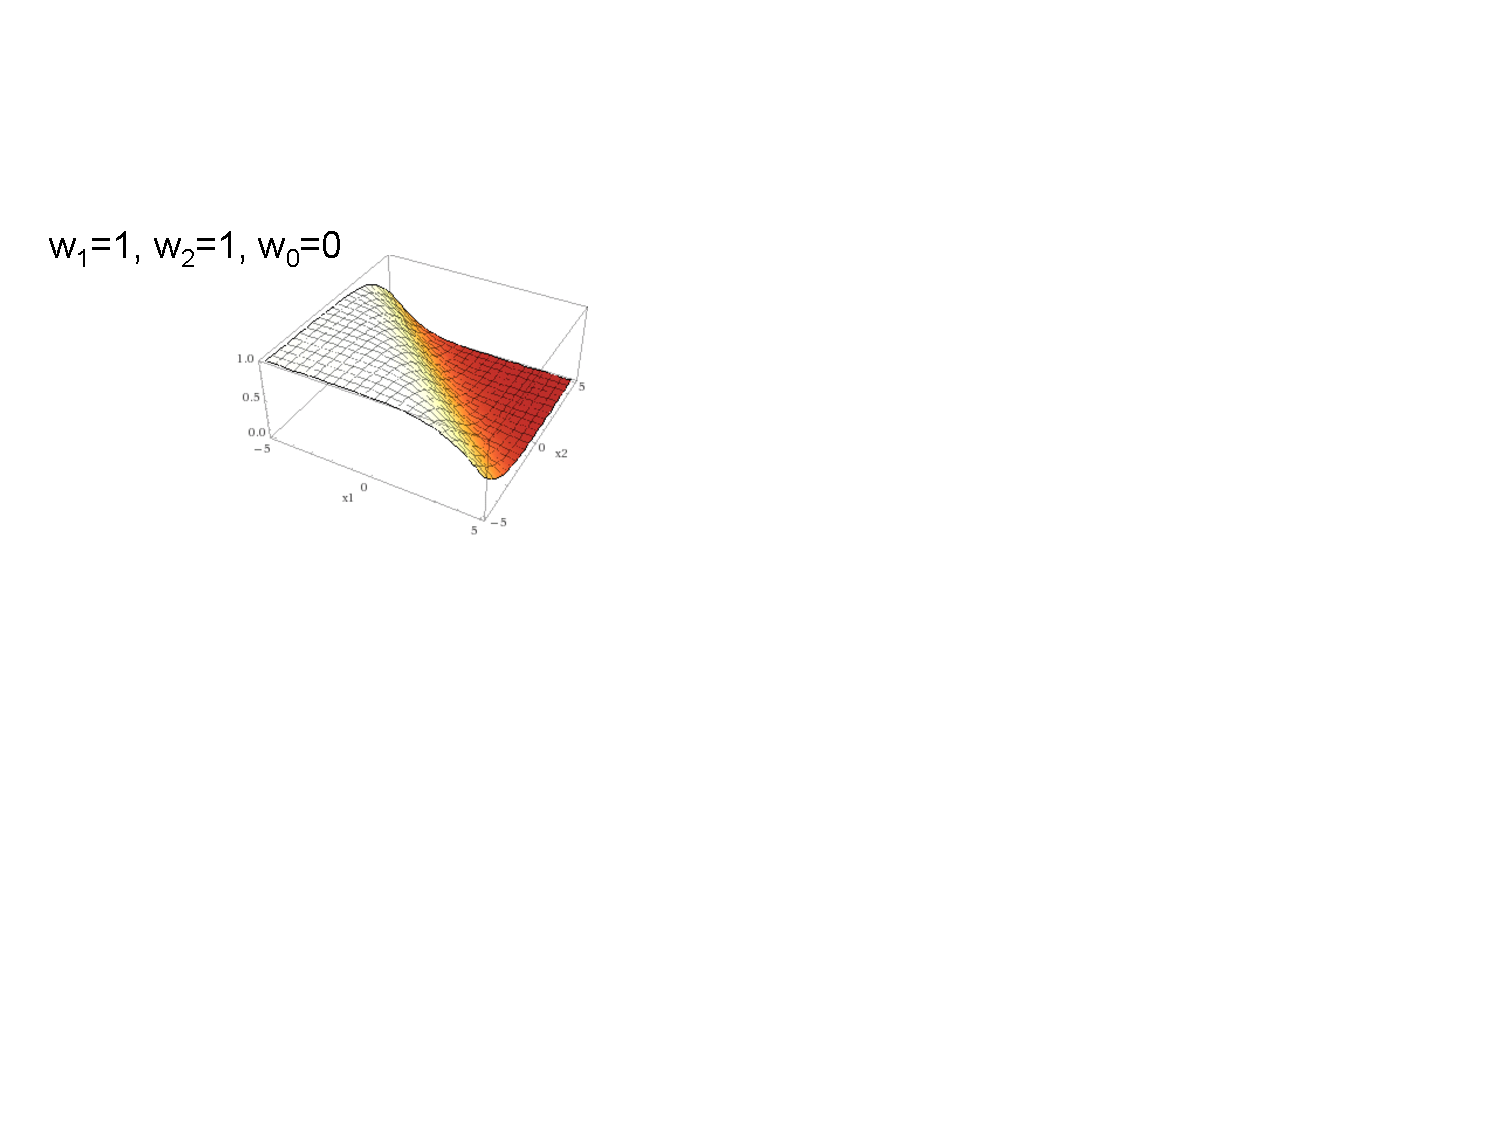
\includegraphics[width=2in]{figures/decision_boundary_example-2D.pdf}   \hfill \\

$P(Y=0 | X, w)$ decreases as $w_0 + \sum_i w_i x_i$ increases. 
Again, if you set the stuff inside the exponential to zero, you get the decision boundary hyperplane.

\subsubsection{Finding the w coefficients}
Generative (Naive Bayes) loss function: 
Now $j$ is a data point with observations indexed over $i$.


\begin{align*}
	\ln P(D | \bm{w}) = \sum_{j=1}^N  &  \ln P(x^j, y^j | \bm{w}) \mbox{   } \mbox{    (the full log-likelihood)}\\
					& \mbox{use Bayes' rule to rewrite conditionally}  \\  % J added this line. 
					= \sum_{j=1}^N  &  \ln [P(y^j | x^j, \bm{w}) P(x^j | \bm{w})] \\ % J added this line. 
				=  \sum_{j=1}^N  & \ln P(y^j | x^j , \bm{w}) + \sum_{j=1}^N \ln P(x^j | \bm{w})
\end{align*}

We decide to ignore the 2nd term because it won't help you get better predictions for that data anyway. 
Or, "From a machine learning perspective, "God gave us the data" and we don't care about the 2nd sum."  % Erick 2/6/2016

Professor Farhadi is calling this first time a discriminative (logistic regression) loss function:  \hfill \\
It is helping you discriminate between different classes.  It's not going to help you model the data. 
This is unlike regression; we don't care about the value it puts out.  We only care about what the resulting class is.  \hfill \\

% Erick. 
This is the difference between statistics and machine learning.  We only care about getting the best $\bm{w}$ for discriminating between classes. 

\textbf{Conditional Data Likelihood:} 
"Conditional" because you are conditioning on what $\bm{X}$ is. 
\begin{align*}
	\ln P(D_Y | D_{\bm{X}}, \bm{w}) = \sum_{j=1}^N \ln P(y^j | \bm{x}^j, \bm{w})
\end{align*}
$D_Y$ = ???  \hfill \\
$D_{\bm{X}}$ = ???   \hfill \\
Doesn't waste effort learning $P(X)$.  Focuses on $P(Y| \bf{X})$, which is all that matters for classification. \hfill \\
Discriminative models cann't compute $P(\bm{x}^j | \bm{w})$!  ??? 
\hfill \\

\subsubsection{Conditional Log Likelihood}
Just need to figure out how to go up and find the maximum likelihood. 

(the binary case only).  \hfill \\
$P(Y=0 | \bm{X}, \bm{w}) = \frac{1}{1 + \exp(w_0 + \sum_i w_i X_i)}$  \hfill \\
$P(Y=1 | \bm{X}, \bm{w}) = \frac{\exp(w_0 + \sum_i w_i X_i)}{1 + \exp(w_0 + \sum_i w_i X_i)}$  \hfill \\

($ l( \bm{w} )$ is conditional data log-likelihood.)  
\begin{align*}
	l( \bm{w})  \equiv  &  \sum_j \ln P(y^j | x^j, \bm{w})  \\
	& \mbox{Since $y^j$ is in \{0, 1\}, sum over the two cases: }   \\
	& \mbox{(the $y^j$ and $(1-y^j)$ act like delta functions)}   \\
	l(\bm{w})  =  & \sum_j y^j \ln P(y^j = 1 | x^j, \bm{w}) +(1 - y^j) \ln P(y^j = 0 | x^j, \bm{w})  \\
	& \mbox{plug in the definition of the likelihoods and do algebra to get:}  \\
	=& \sum_j  y^j (w_0 + \sum_i^n w_i x_i^j)  - \ln(1 + \exp(w_0 + \sum_i^n w_i x_i^j)) 
\end{align*}	

While we can't find a closed-form solution to optimize $l(\bm{w})$,  $l(\bm{w})$ is concave so we can to gradient \underline{as}cent. 
Jsut need to figure out how to go up and find the maximum likelihood.   % Wk 5 audio

\subsubsection{Gradent ascent to optimize w}
To maximize, we can't take derivative w.r.t $\bm{w}$ and optimize b/c no closed form solution.  % Wk 5 audio 
Instead we form the gradient vector and move along the gradient. % Wk 5 audio
Conditional likelihood for Logistic Regression is convex.  (see above)  \hfill \\
In this case it doesn't matter b/c we have a concave function.  % Wk 5 audio
Iterate to find $\bm{w}$: start somewhere, find gradient direction, make step in that direction, repeat, repeat.
\hfill \\

\textbf{Gradient}:  gives ascent or descent direction. \hfill \\
\begin{align*}
	\nabla_w l(\bm{w}) = [\frac{\partial l(\bm{w})}{\partial w_0}, \dots, \frac{\partial l(\bm{w})}{\partial w_n}]'  \hfill \\
\end{align*}
	(The $'$ at the end is for transpose b/c usually a column vector.)  \hfill \\
\textbf{Update Rule:} \hfill \\
\begin{align*}
	\Delta \bm{w} &= \eta \nabla_{\bm{w}} l(\bm{w})
\end{align*}
$\eta$ is the learning rate.  $\eta > 0$.  
	It can't be too big or you can get lost.  
	It can't be too small or you take forever to converge. 

Your next weights $(t+1)$ become: 
$w_i^{(t+1)} \leftarrow w_i^{(t)} + \eta \frac{\partial l(\bm{w})}{\partial w_i}$   \hfill \\
\hfill \\
Gradient ascent is the simplest  of optimization approaches.  
Note that conjugate gradient ascent is much better (see reading).(?)  \hfill \\

See slides for derivation of: \hfill \\
$\displaystyle \frac{\partial l(w)}{\partial w_i} = \sum_j x_i^j (y^j - P(Y^j = 1 | x^j, w))$

\subsubsection{Example of gradient ascent to maximize conditional log likelihood}
(M(C)LE; C for conditional) \hfill
Learning an approximation of the step function.  % Wk 5 audio. 

Use the equations: \hfill \\
\begin{itemize}
	\item \textbf{eq 1:} $w_i^{(t+1)} \leftarrow w_i^{(t)} + \eta \frac{\partial l(\bm{w})}{\partial w_i}$
	\item \textbf{eq 2:} $\displaystyle \frac{\partial l(w)}{\partial w_i} = \sum_j x_i^j (y^j - P(Y^j = 1 | x^j, w))$
			 The loss function is conditional on log likelihood.  % Wk 5 audio
	\item \textbf{eq 3:} $P(Y=1 | X, W) = \frac{\exp(w_0 + \sum_i w_i X_i)}{1 + \exp(w_0 + \sum_i w_i X_i)}$
	\item \textit{note:} superscript is for the $j^{th}$ data point and 
			subscripts are for the $i^{th}$ value of the input ($x$) array.  
			Don't forget that there is an $i=0$ $(x_0 = 1)$ bias term. 
\end{itemize}
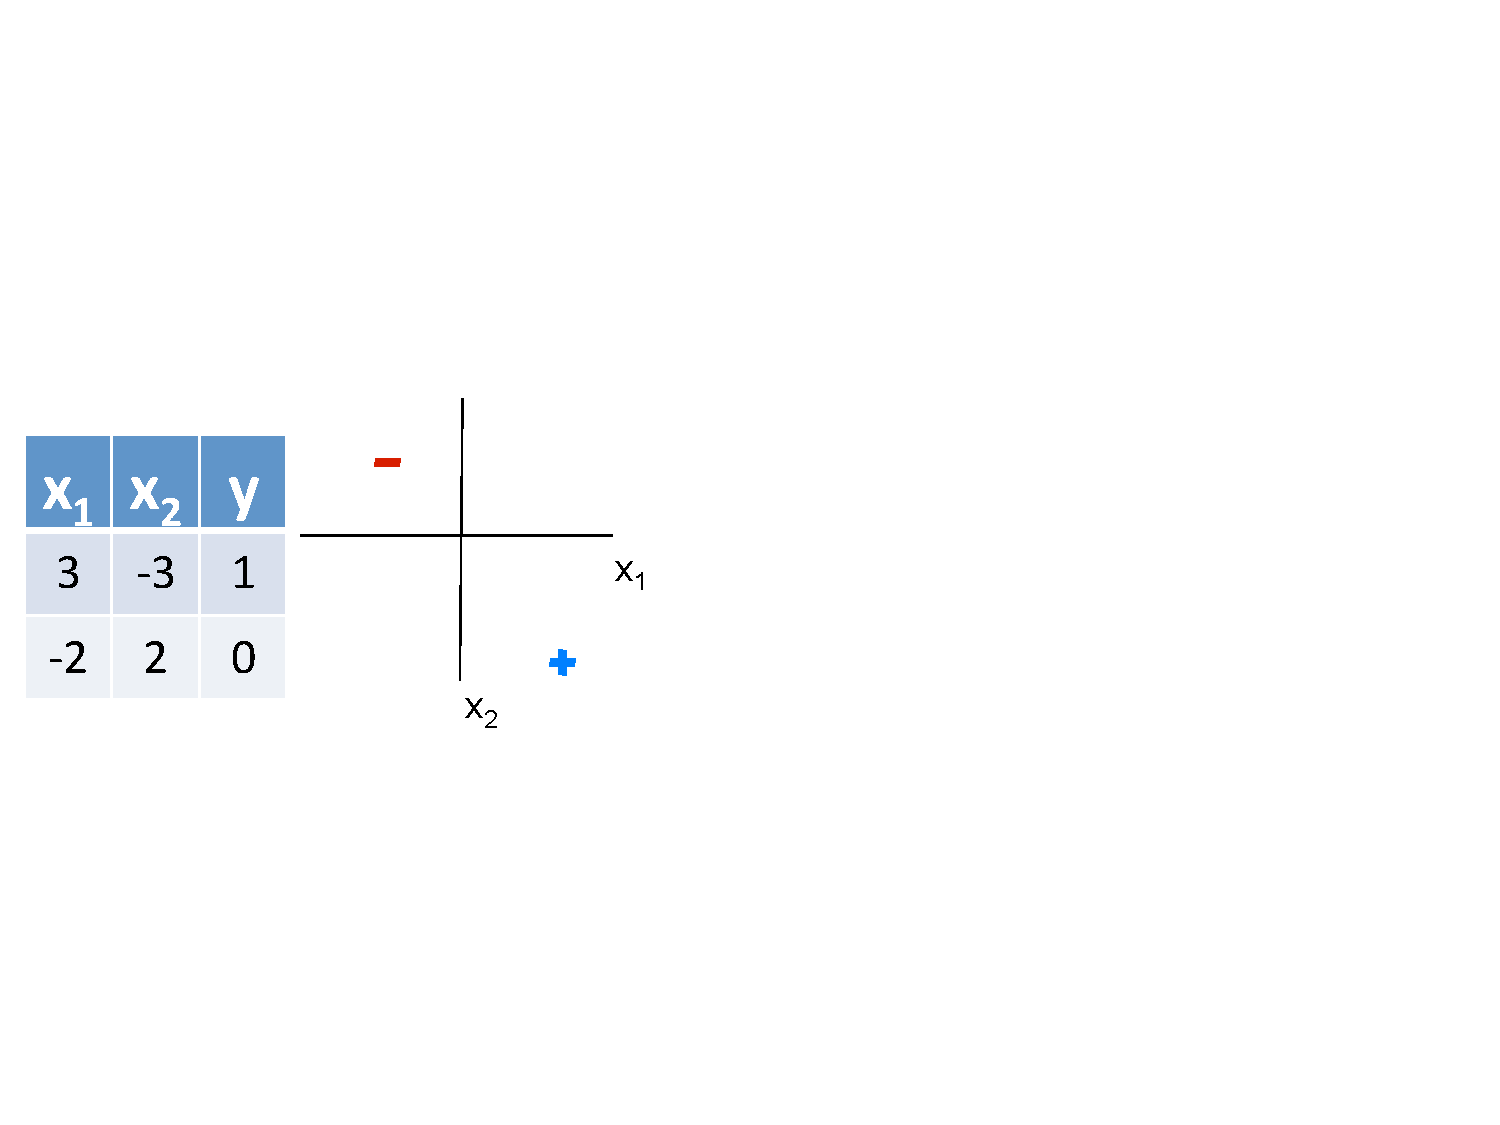
\includegraphics[width=1.5in]{figures/gradient_ascent_logistic_regression.pdf}   \hfill \\
\begin{itemize}
	\item begin with t=0 and $w = [w_0 + w_1 + w_2] = [0, 0, 0]$
	\item calculate \textbf{eq 3} for each Y.  
		\begin{itemize}
			\item For j = 0:  
				\begin{align*}
					P(Y^0 = 1 | x^0, w) &= \frac{\exp(0 + 0*3 + 0^(-3))}{(1 +  \exp(0 + 0*3 + 0*(-3)))} \\
						&= 1/(1+1) = 1/2
				\end{align*}
			\item For j = 1:  
				\begin{align*}
					P(Y^1 = 1 | x^1, w) &= \frac{\exp(0 + 0*(-2) + 0^(2))}{(1 +  \exp(0 +  0*(-2) + 0^(2)))} \\
						&= 1/(1+1) = 1/2
				\end{align*}
		\end{itemize} 
	\item calculate the terms that go into \textbf{eq 2} by looping over the 3 values of $i$ (bias and two other coefficients) and 2 values of $j$ (2 data points).  
		\begin{itemize}
			\item for $i=0, j=0$: ($j=$0th (1st) training example, bias term) \hfill \\
				 $x_0^0(y^0 - P(Y^0=1|x^0, w)) = 1(1-0.5) = 0.5$ 
			\item for $i=0, j=1$: ($j=$1st (2nd) training example, bias term) \hfill \\
				 $x_0^0(y^0 - P(Y^0=1|x^0, w)) = 1(0-0.5) = -0.5$ 
			
			\item for $1=1, j=0$: ($j=$0th (1st) training example, $x_1$ term) \hfill \\
				 $x_1^0(y^0 - P(Y^0=1|x^0, w)) = -2(1-0.5) = 1.5$ 
			\item for $i=1, j=1$: ($j=$1st (2nd) training example, $x_1$ term) \hfill \\
				 $x_1^1(y^1 - P(Y^1=1|x^1, w)) = -2(0-0.5) = 1.0$ 
				 
			\item for $1=2, j=0$: ($j=$0th (1st) training example, $x_2$ term) \hfill \\
				 $x_2^0(y^0 - P(Y^0=1|x^0, w)) = -3(1-0.5) = -1.5$ 
			\item for $i=2, j=1$: ($j=$1st (2nd) training example, $x_2$ term) \hfill \\
				 $x_2^1(y^1 - P(Y^1=1|x^1, w)) = 2(0-0.5) = -1.0$ 
		\end{itemize}
	\item Now we can compute the gradient (\textbf{eq 2}):
		\begin{itemize}
			\item $\nabla_w l(\bm{w}) = [\frac{\partial l(w)}{\partial w_1}, \frac{\partial l(w)}{\partial w_2}, \frac{\partial l(w)}{\partial w_3}]$
				\begin{align*}
					%\frac{\partial l(w)}{\partial w_i} &= \sum_j x_i^j (y^j - P(Y^j = 1 | x^j, w)) \\
						&= [0.5 - 0.5, 1.5 + 1.0, -1.5 - 1] = [0, 2.5, -2.5]
				\end{align*}
		\end{itemize}
	
	\item Use $\eta = 0.1$ to scale the gradient:  (\textbf{eq 1}) \hfill \\
			$w = [0,0,0] + 0.1*[0, 2.5, 2.5] = [0, 0.25, -0.25]$
	\item Start over with \textbf{eq 3} and updated $w$.
		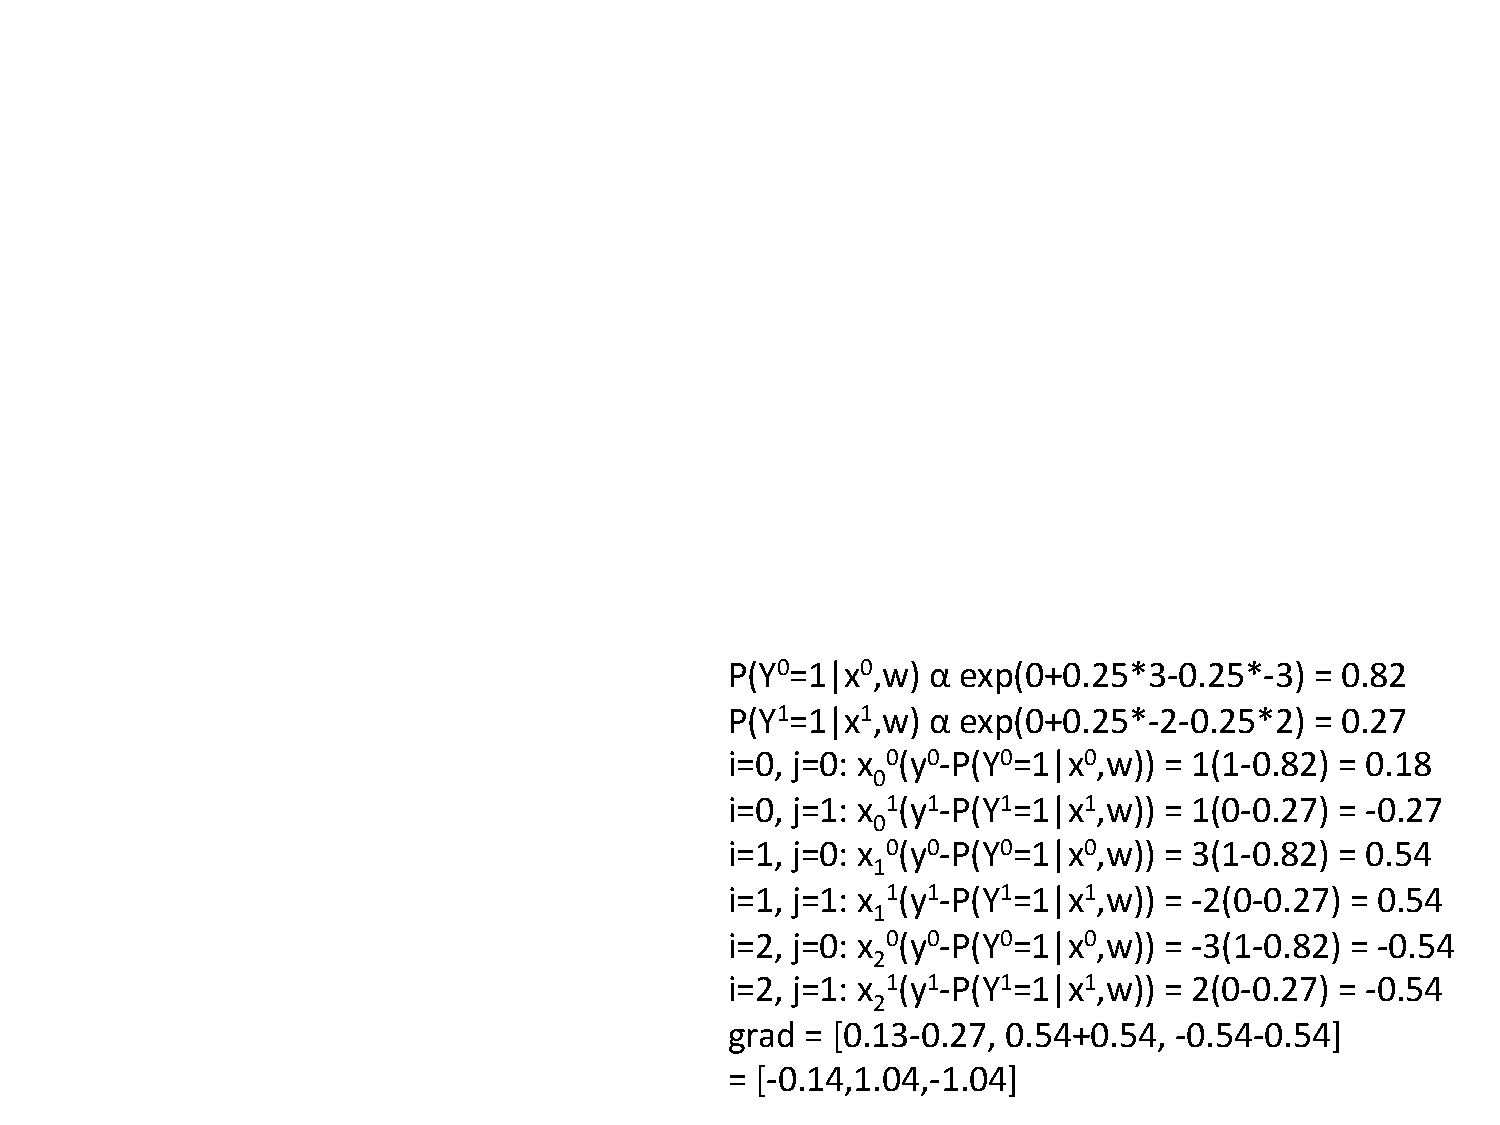
\includegraphics[width=2in]{figures/logistic_regression_ex_loop_2.pdf}
\end{itemize}

How to do more algorithmically:  \hfill \\
You don't have to get all the info to update all the weights at once.  
Do them one at a time.  \hfill \\
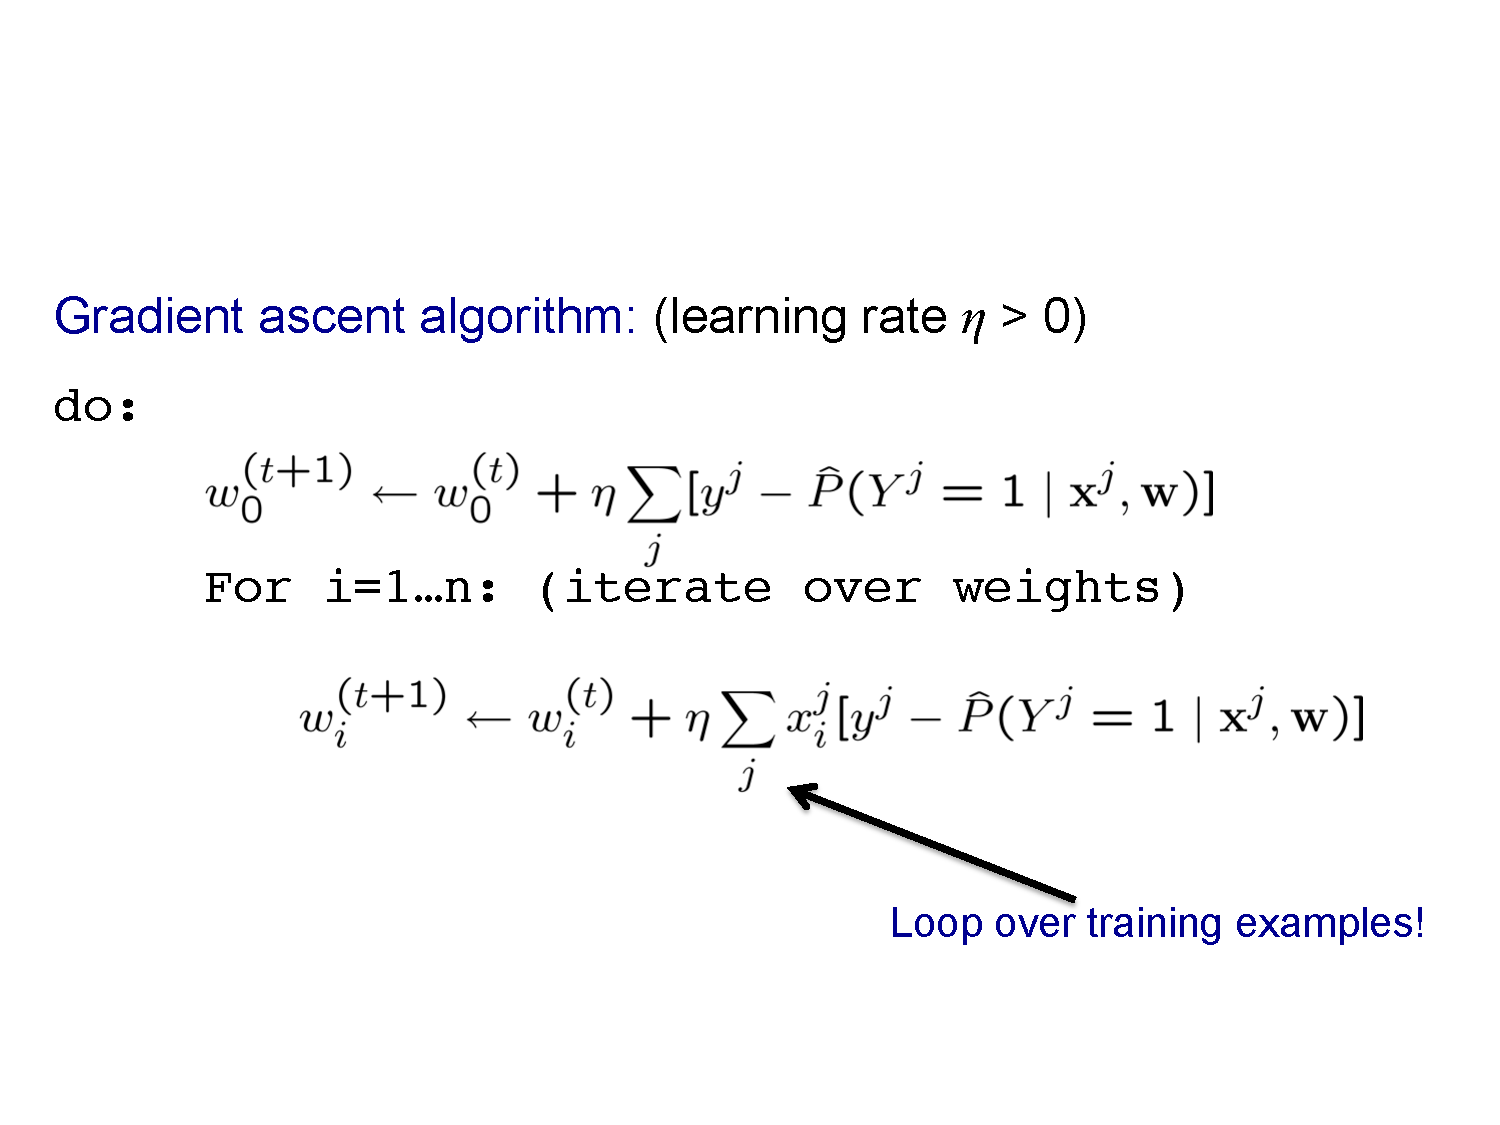
\includegraphics[width=2.5in]{figures/gradient_descent_algorthim.pdf}

\underline{How do you decide when to stop?} \hfill \\
(Not in notes!) \hfill \\

You need a criteria that tells you when to stop updating your gradient. 
	Use a threshold for magnitude of the gradient. 
	When the amount of change is small it is not changing a lot.  If concave, you are close to global optima. 

Why don't we wait until it gets to zero? 
	The chances of us hitting zero is low, and we might spend a lot of time wasting CPU cycles on negligible changes. 
	
When we are really far from the global optimum we can afford to take bigger steps. 
	Think about the objective function.  We can afford to make big steps if we are far.  
	If we make big steps when close, we can get farther away .

You could use this policy: let $\nu$ be big at the beginning of a loop counter. 
	Increase the value until you see a drop.
	"Line search" asks "what is maximum value of this parameter that gives you no drop?"  


\subsubsection{Overfitting in Logistic Regression}

 
 \underline{Intro \#1:}  \hfill \\
Be weary of large parameters.  % Audio wk 5
	Large parameters (large $a$ in $\frac{1}{1 + exp(-a)}$) lead to a step function.  
	That's ok if you truly want a step, but you should be concerned about overfitting the minute you see a large parameter.
	We could regularize again: apply a penalty for large parameters. 
    	Could do something like maximizing $w^* = \argmax_w l(w) - \lambda*(||w||_2^2)$ insead of $w* =  argmax_w l(w)$. 
	But that's not ideal.  Might have a hard time optimizing value of \_\_\_.  \hfill \\
	
Instead, use a probabilistic way of regularization.
	We've done this before using a prior.  Instead of MLE, we did MAP. The prior regularizes. 
	What would be the form of our prior be? 
	$P(Y|X,w)P(w)$ ??.
	
How did we write that eqiaton down?  Write sigmoid shape.  Write as a parametric function w/ parameter w. 
Whenever we pick a form for that $P(Y|X,w)P(w)$, we need to be careful with the form we do for that $P(w)$ b/c we want to take a derivative. 
What is the form of $P(Y|X,w)$?  Is of form $e^{something}$
 
 \underline{Intro \#2:}   \hfill \\
 
Like in linear regression, the maximum likelihood solution prefers higher weights.  
Higher weights can give higher likelihood of properly classifying examples close to the decision boundary.  
This over-fitting causes features to have larger influences on the decision:  \textbf{beware of overfitting!!!}. 
Again, you can use regularization to penalize high weights.
This will be covered more later. 
\hfill \\

\subsubsection{MAP for Logistic Regression}
Above was M(Conditional)LE.     \hfill \\
Recall that the MAP/MLE difference is \_\_\_\_\_\_\_\_\_.  \hfill \\
Priors on $\bm{w}$ are commonly added for regularization.    \hfill \\
Helps avoid very large weights and overfitting.    \hfill \\
$P(\bm{w} | Y, \bm{X}) \propto P(Y, | \bm{X}, \bm{w} ) P(\bm{w} )$  \hfill \\
Use a normal distribution with zero mean and "identity covariance".  (\_\_\_\_):  \hfill \\
$ \displaystyle  P(\bm{w} ) = \prod_i \frac{1}{\kappa \sqrt{2 \pi}} e^{\frac{-w_i^2}{2 \kappa^2}}$ \hfill \\
\hfill \\

MAP estimate: 
\begin{align*}
	w* &= \argmax_w \ln[P(\bm{w}) \prod_{j=1}^N P(y^j | x^j, \bm{w})]  \\
		&= \argmax_w \ln[ \prod_i \frac{1}{\kappa \sqrt{2 \pi}} e^{\frac{-w_i^2}{2 \kappa^2}}   \prod_{j=1}^N P(y^j | x^j, \bm{w})]
\end{align*}
Add $\log P(\bm{w})$ to the objective:
\begin{align*}
	\ln P(\bm{w}) & \propto - \frac{\lambda}{2} \sum_i w_i^2 \\
	\frac{\partial \ln P(\bm{w})}{\partial w_i} &= \lambda w_i
\end{align*}
This is a quadratic penalty (???) that drives the weights toward zero. \hfill \\
It adds a negative linear term to the gradients (???).  \hfill \\
Also applicable in linear regression! 

\subsubsection{Review: MLE vs. MAP for Logistic Regression}
\underline{Maximum conditional likelihood estimate:}
\begin{align*}
	w* &= \argmax_w \ln[\prod_{j=1}^N P(y^j | x^j, \bm{w})] \\
	w_i^{(t+1)} & \leftarrow w_i^{(t)} + \eta \sum_j x_i^j [y^j - \widehat{P}(Y^j = 1 | x^j, \bm{w})]\\
\end{align*}

\underline{Maximum conditional a posteriori estimate:}
\begin{align*}
	w* &= \argmax_w \ln[P(\bm{w}) \prod_{j=1}^N P(y^j | x^j, \bm{w})] \\
	w_i^{(t+1)} & \leftarrow w_i^{(t)} + \eta \{ -\lambda w_i^{(t)} +  \sum_j x_i^j [y^j - \widehat{P}(Y^j = 1 | x^j, \bm{w})]\\
\end{align*}

\hfill \\  \hfill \\


Vocab \hfill \\
\begin{itemize}
	\item \textbf{discriminative}:  estimates joint probabilities.  E.g. $p(Data, Zebra)$, $p(Data, No Zebra)$. 
	\item \textbf{generative}:  E.g. $p(Zebra | Data)$, $p(No Zebra | Data)$. 
\end{itemize}

\subsubsection{Multiclass Logistic Regression (discrete labels)}
Define a weight vector $w_i$ for each $y_i$ where i ranges from $1$ to $R-1$ for $R$ classes.
You don't need a weight vector for the $R^{th}$ class b/c its probability is 1 - the sum of the rest.  \hfill \\
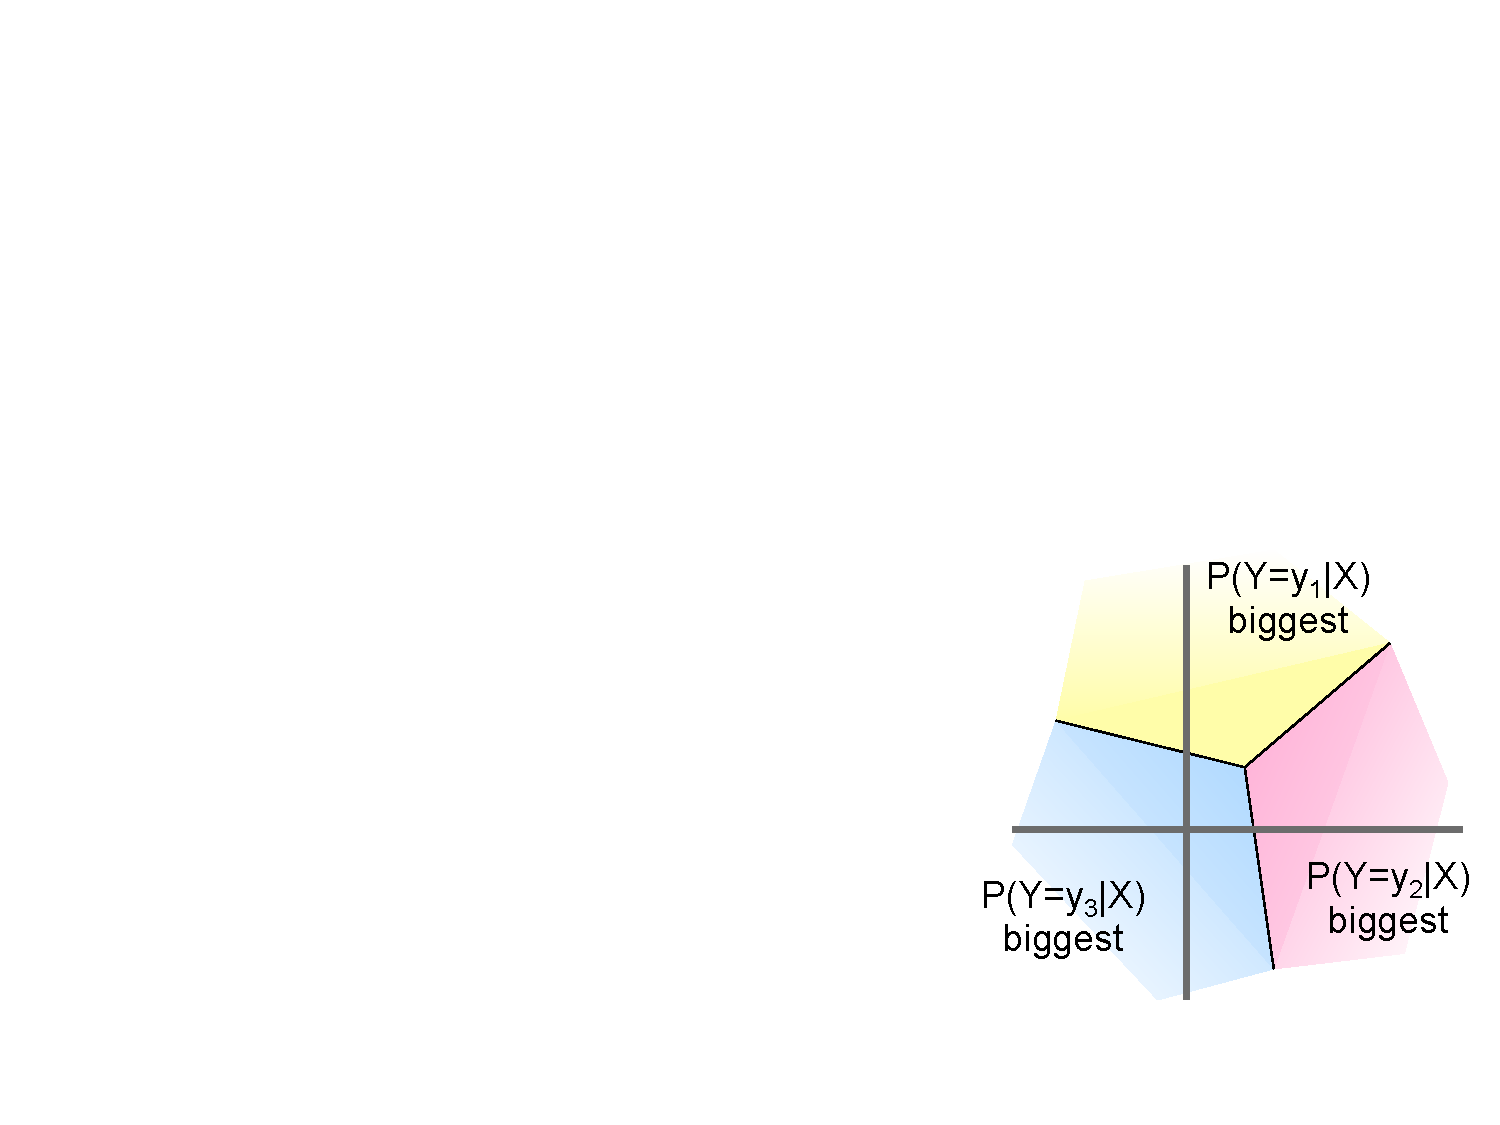
\includegraphics[width=1in]{figures/multiclass_logistic.pdf} \hfill \\
\begin {align*}
	P(Y=1 | X ) & \propto \exp(w_{10} + \sum_i w_{1i}X_i)  \\
		& \mbox{note: $\bm{w}$ is now a matrix, not an array.}  \\
	P(Y=2 | X ) & \propto \exp(w_{20} + \sum_i w_{2i}X_i)  \\
	 & \dots \\
	 & \mbox{the last probability is defined relative to the rest.}  \\
	P(Y=r | X ) &= 1- \sum_{j=1}^{r-1} P(Y=j | X)
\end{align*}
After normalizing, your probabilities become: 
\begin {align*}
	P(Y=y_k | X ) &=  \frac{\exp(w_{k0} + \sum_{i=1}^n w_{ki} X_i)}{1 + \sum_{j=1}^{R-1} \exp(w_{j0} + \sum_{i=1}^n w_{ji}X_i)} \\
	& \mbox{the last class is 1 - the sum of the other probabilities:} \\
	P(Y=y_R | X ) &=  \frac{1}{1 + \sum_{j=1}^{R-1} \exp(w_{j0} + \sum_{i=1}^n w_{ji}X_i)} 
\end{align*}
Note: features can be discrete or discontinuous. 

\subsubsection{Gaussian Naive Bayes vs Logistic Regression.}
Gaussian Naive Bayes with class-independent variances is representationally equivalent to Linear Regression.
("If you do have an infinite number of training examples, the GNB and LR produce identical classifiers.")  % Erick 2/7
The solutions different because of the objective (loss) function.  \hfill \\

If you do have class-independent variances and the underlying model is gaussian, GNB does better than LR.
You get an incorrect model for GNB if you don't have class-independent variances.  %Erick
LR is less biased because it does not assume conditional independence.  % Erick.
 \hfill \\  \hfill \\

You could use either to learn $ f: X \rightarrow Y$ for $X$ that is a vector of real-valued features ($< X_1, \dots, X_n >$) and boolean Y. \hfill \\ \hfill \\

The two approaches make different assumptions:   \hfill \\
\begin{itemize}
	\item NB assumes features are independent given the class.  This is an assumption on $P(\bm{X} | Y)$.
	\item LR assumes functional form of $P(Y|\bm{X})$, and makes no assumption on $P(\bm{X} | Y)$.
\end{itemize}

Gaussian Naive Bayes classifier would assume: \hfill \\
\begin{itemize}
	\item all $X_i$ are conditionally independent given Y.  
		If you fix what hump you are looking at, you don't need to worry about the rest of the parameters. 
	\item model $P(X_i | Y = y_k)$ as Gaussian with $N(\mu_{ik}, \sigma_i)$.  (Your inputs are each produced by a gaussian.)
	\item model $P(Y)$ as Bernoulli$(\theta, 1-\theta)$
\end{itemize} 
This implies the form of $P(Y|X)$ is:
$\displaystyle P(Y=1 | X= < X_1, \dots, X_n >) = \frac{1}{1 + \exp(w_0 + \sum_i w_i X_i)}$. \hfill \\
In the slides, he derives the form.   \hfill \\
(??)  You see that if you assume Gaussian in Logistic Regression, you get: \hfill \\
 $w_0 = \ln \frac{1 - \theta}{\theta} + \frac{\mu_{i0}^2 + \mu_{i1}^2}{2 \sigma_i^2}$ and $w_i = \frac{\mu_{i0} + \mu_{i1}}{\sigma_i^2}$
 
 His confusing summary: \hfill \\
 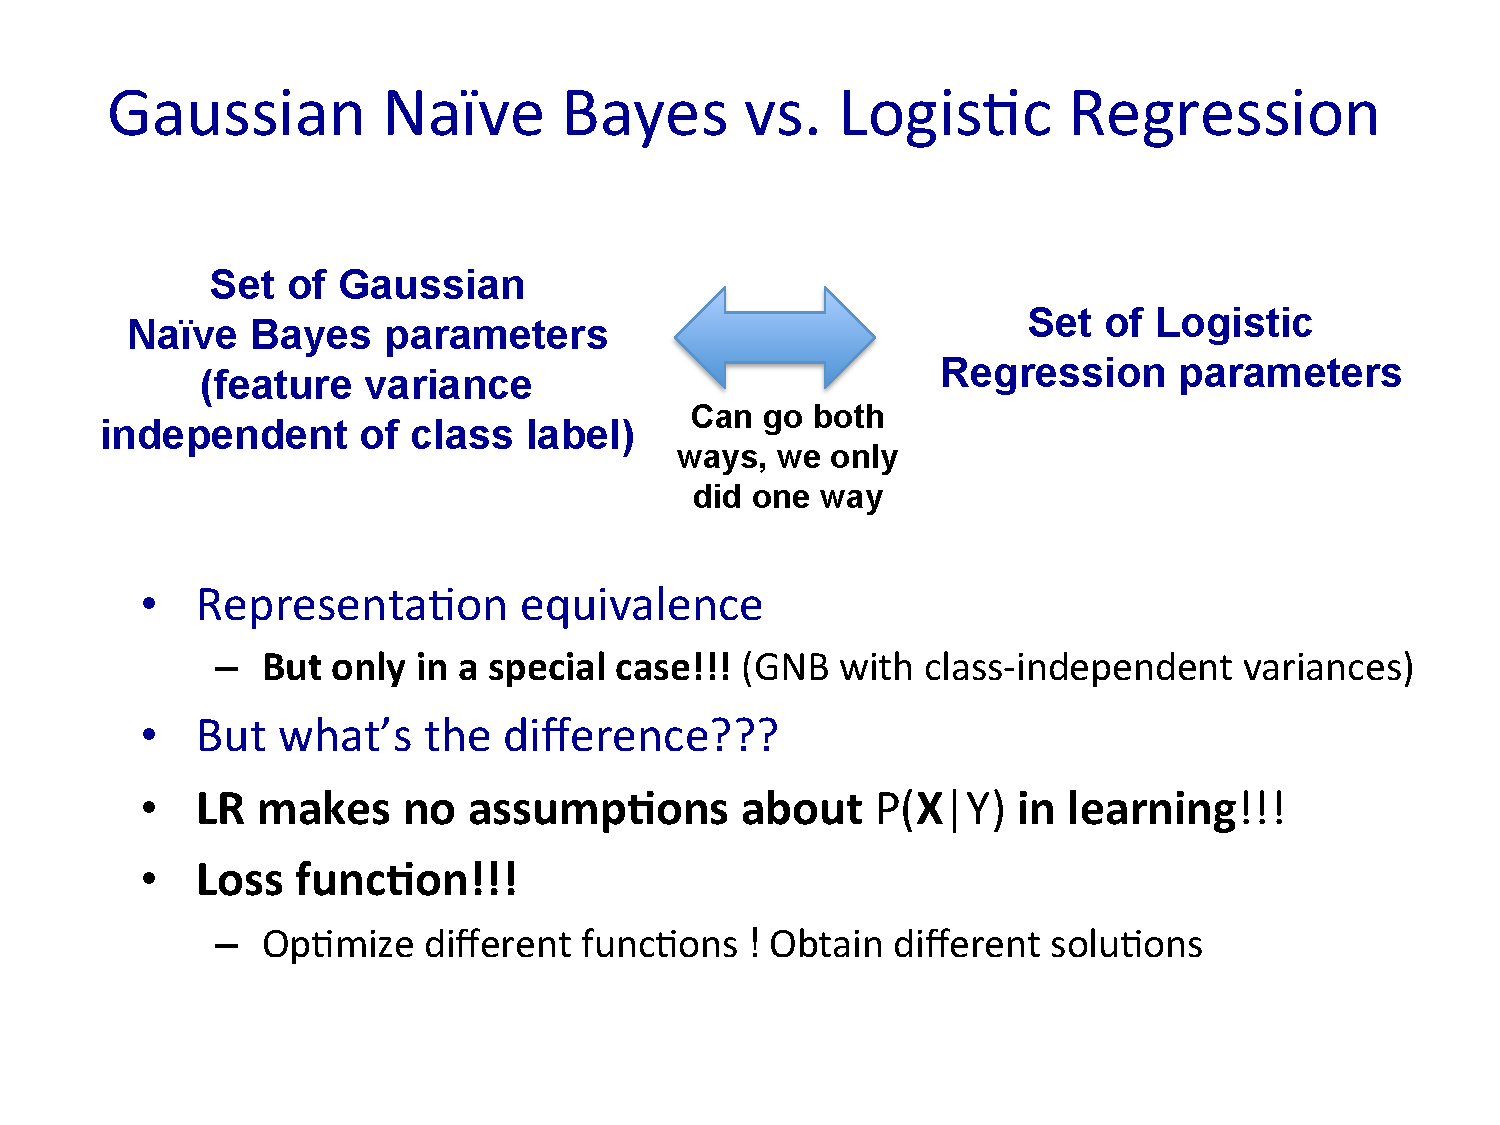
\includegraphics[width=2.5in]{figures/GNB_vs_LR.pdf}
 Attempted translation: 
 
 Note: you need more parameters to train Naive Bayes. \hfill \\
 $4n + 1$ parameters for GNB,  $n + 1$ parameters for Logistic Regression. \hfill \\
 The NB parameter estimates are uncoupled, so there are more of them.   \hfill \\
 (The Logistic Regression parameter estimates \underline{are} coupled.)

If you don't have infinite data (? "non-asymptotic analysis"): \hfill \\
For $n$ attributes in $X$, NB needs $O(\log n)$ samples to converge and Logistic Regression needs $O(n)$.  
So GNB converges more quickly to its (perhaps less helpful) "asymptotic estimates."

You have to do all of the optimization at once, all together if you are doing logistic regression.  ???
Easier in a certain sense to fit a Gaussian model. 
Typically we have a lot of data, and that data is not gaussian so Logistic Regression is probably better. 

\subsubsection{Andrew Ng}
* gives numbers between 0 and 1 (good for classification)   \hfill \\
* called "logistic regression" but it is really for classification.  (don't be confused by "regression") \hfill \\
* "sigmoid function" and "logistic function" are essentially synonomous.  \hfill \\
 


\section{Perceptrons}
\smallskip \hrule height 2pt \smallskip

\begin{itemize}
	\item Decision mechanism: sign of $w \cdot x$.  If + say yes, if - say no.  % week 6 audio
	\item Linear classifier in feature space.
	\item Error driven, not probabilistic. \hfill \\
		\begin{itemize}
			\item Mistake driven rather than model drive. \hfill \\
			\item Parameters from reactions to mistakes  % end of slide set 7
		\end{itemize}
	\item does better with linearly separable data. 
	\item Parameters are from a discriminative interpretation % end of slide set 7
	\item To train, you go through the data until the held-out accuracy maxes out. % end of slide set 7
	\item  Just moving the plane to satisfy your labels.
			Then project new sample into this space and see which side it was on.  % week 6 audio
	\item Note you can scale your $w$ (weight) vector(s) by any constant because all you care about is sign($w \cdot x$).
		This rescales your gamma by that constant too! \hfill \\
	\item Bias allows you to have decision boundaries that don't go through the origin.  
		You could us any number, but 1 is used by convention. 
	\item Go through the data point by point, not feature by feature.
		Feature by feature would assume independence of the features (bad).  % Week 6 audio.  
	\item If linearly separable, it will converge.  And we will know how fast it will converge.  % Week 6 audio
\end{itemize}

\subsection{Properties of Perceptron}
\underline{Separability}: some parameters get the training set perfectly correct. \hfill \\
\underline{Convergence}: if the training is separable, the perceptron will eventually converge. \hfill \\
\underline{Mistake Bound}: the maximum number of mistakes (for the binary case) is related to the 
margin or degree of separability: $mistakes \leq \frac{R^2}{\gamma^2}$. \hfill \\
\hfill \\  \hfill \\

Sort of inspired by what might happen in a human brain.
Neurons send info.  A module sums them up \& produces a result. 


\subsection{Problems with the Perceptron}
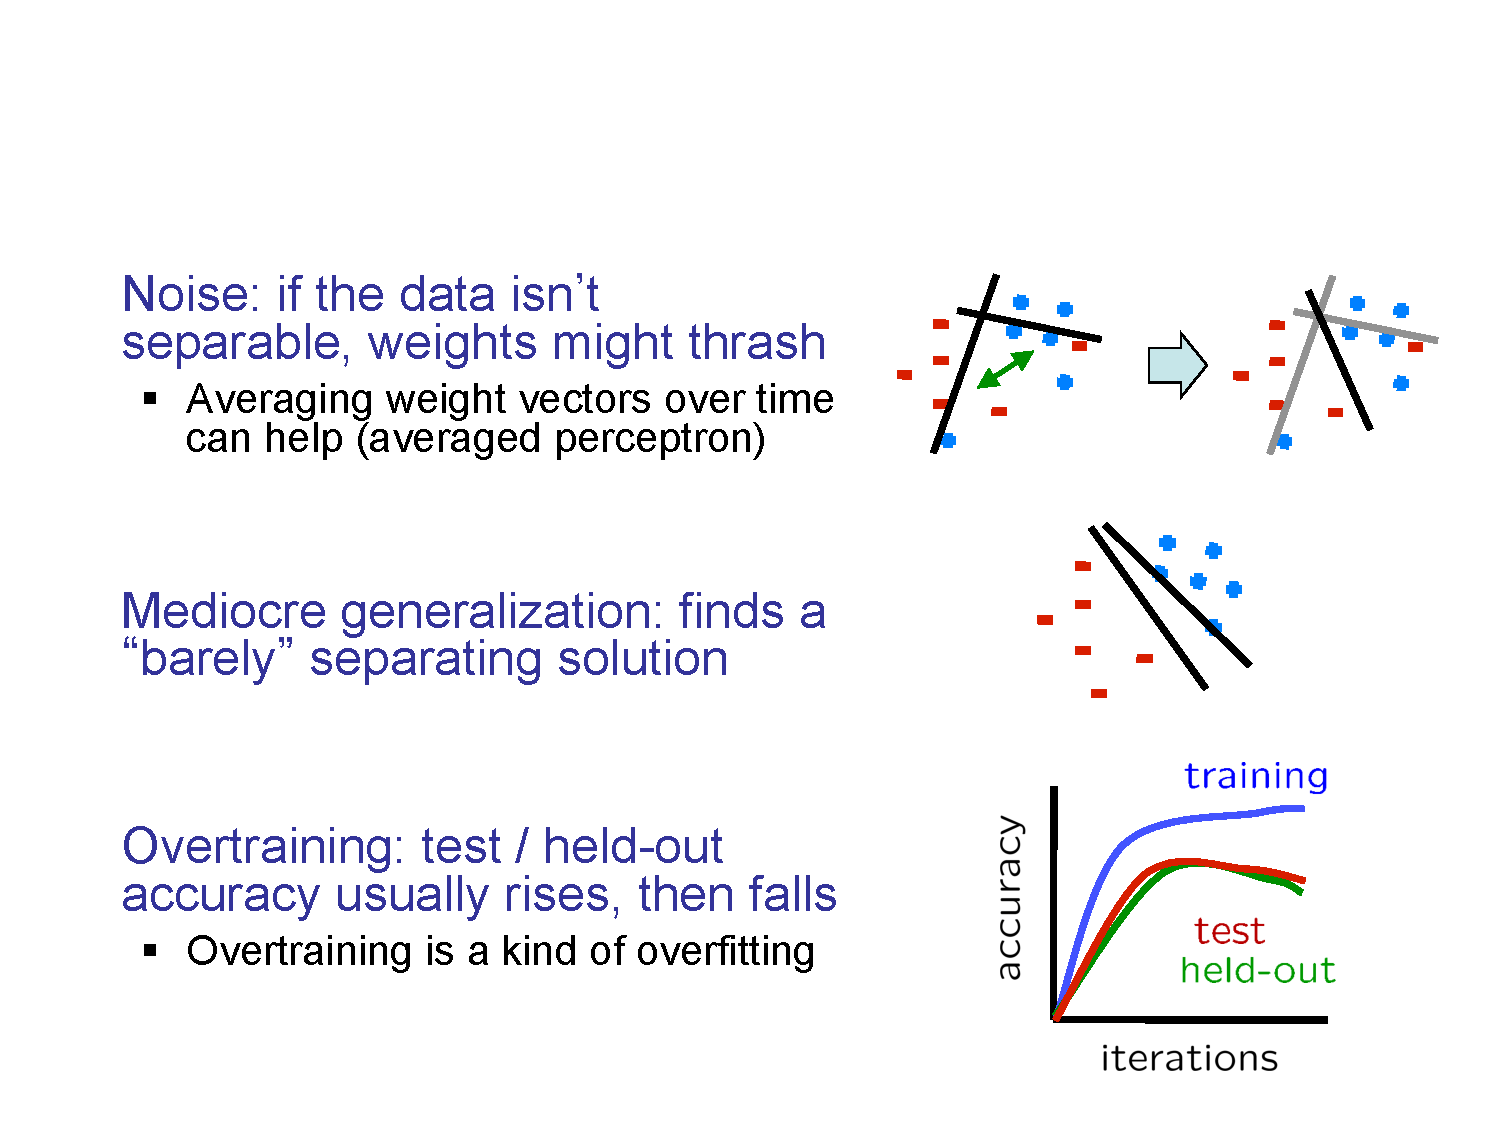
\includegraphics[width=2.8in]{figures/perceptron_problems.pdf}
Lines might not be optimal: issues with generalizibility. \hfill \\
Leads into SVMs. \hfill \\

 \subsection{Linear Classifiers}
 Inputs are feature values.  \hfill \\
 Each feature has a weight.  \hfill \\
 Sum is the activation.  activation$_w(x) = \sum_i w_i x_i = w \cdot x$  \hfill \\
 If the activation is positive, chose output class 1.  \hfill \\
 If the activation is negative, chose output class 2.  \hfill \\
 
 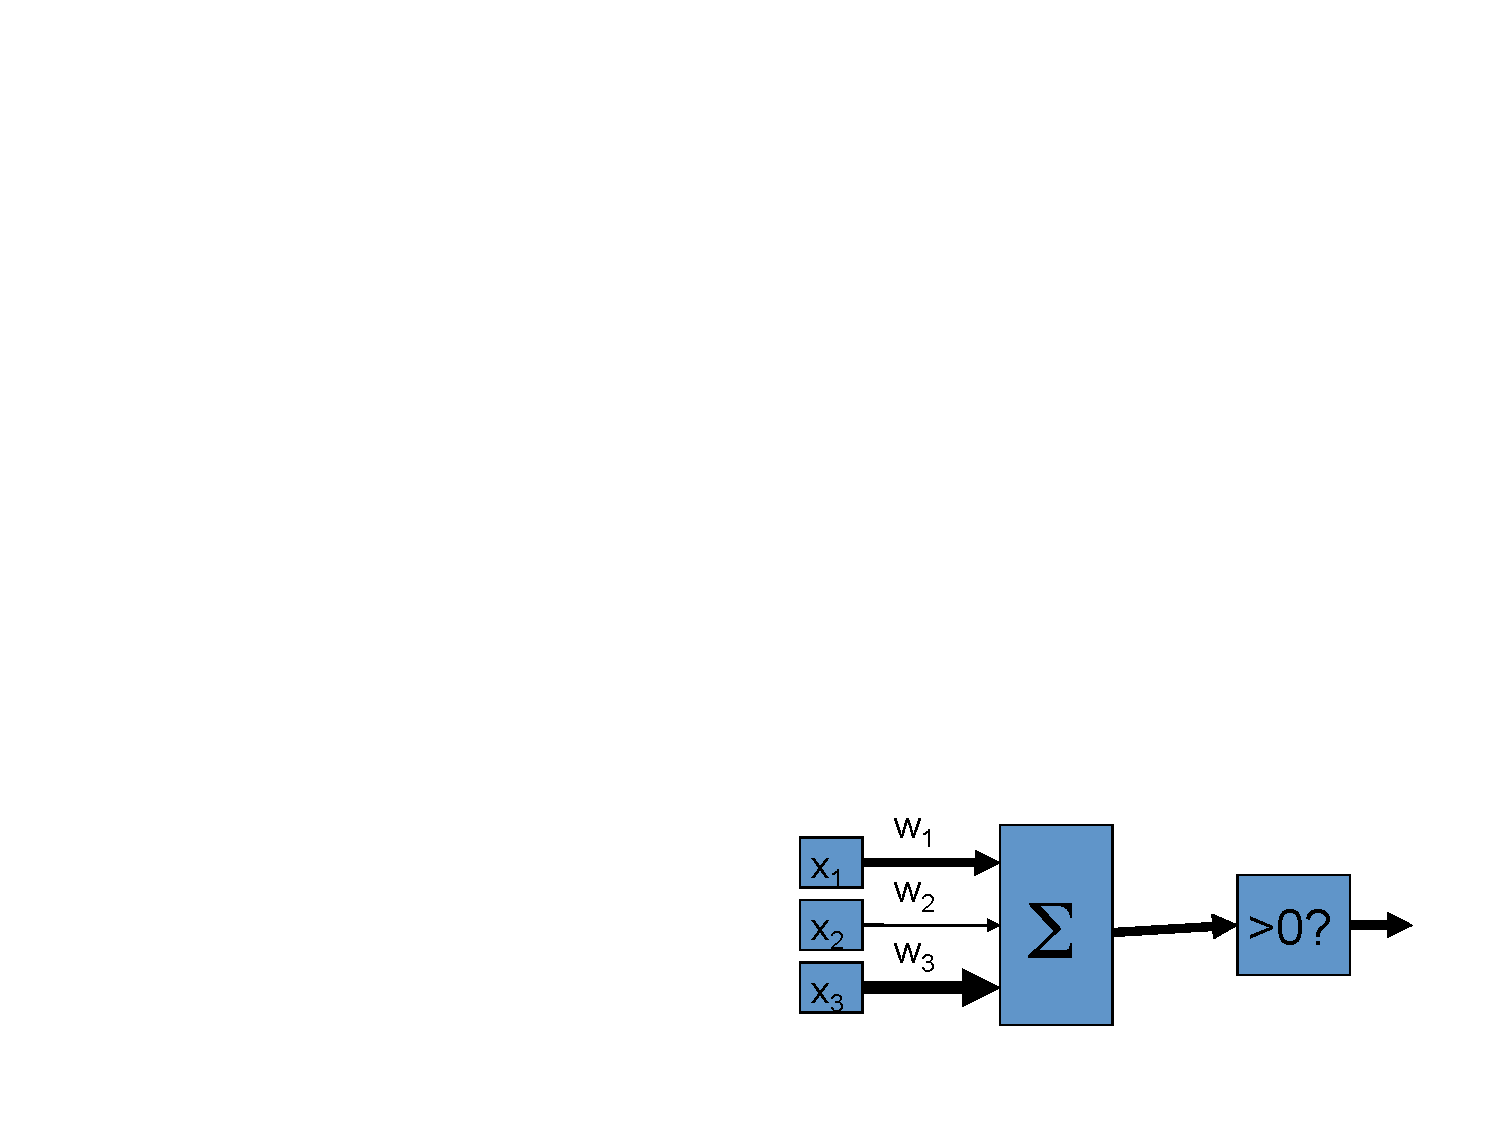
\includegraphics[width=1.5in]{figures/linear_classifier_cartoon.pdf}  \hfill \\
 
 For a binary decision rule:   \hfill \\
 In the space of feature vectors: 
 \begin{itemize}
 	\item examples are points
	\item any weight vector is a hyperplane
	\item one side corresponds to y = +1
	\item the other side corresponds to y = -1
	\item ??? The $w \cdot x = 0$ is the solution to the line.
 \end{itemize}
 
 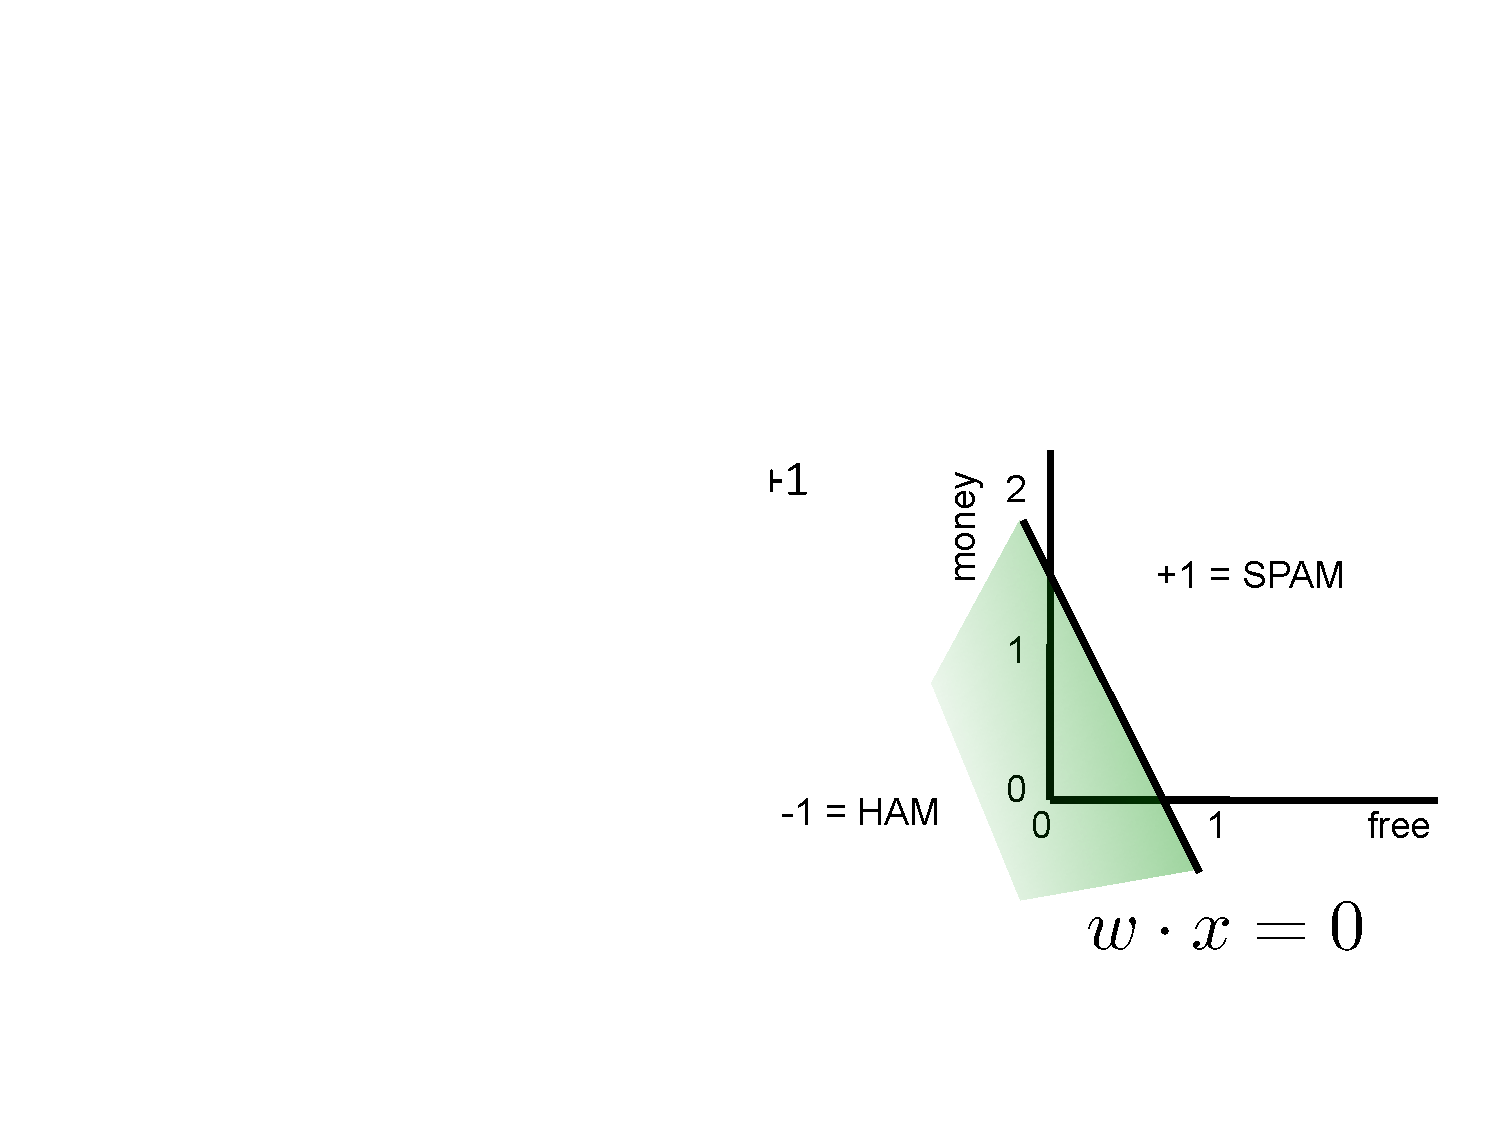
\includegraphics[width=1.5in]{figures/binary_decision_rule.pdf} \hfill \\
 The black line is the decision boundary.     \hfill \\
 $w$ is a vector normal to the decision boundary, and points towards the + label points. 
 
 \subsubsection{Binary Perceptron Algorithm}
 \begin{itemize}
 	\item start with zero weights: $w=0$
	\item for $ t = 1 \dots T$ (T passes over the data):
		\begin{itemize}
			\item for $i = 1 \dots n$ (each training example)
			\begin{itemize}
				\item  Classify with current weights: \hfill \\
					$ y = sign(w \cdot x^i)$ \hfill \\
					(sign($z$)  is $+1$ if $z > 0$, else -1) \hfill \\
				\item if correct (i.e. $y = y^i$), don't change weights.
				\item if it was wrong, update with $w = w + y^i x^i$
			\end{itemize}
		\end{itemize}
 \end{itemize}
Figure showing "you got it wrong:"  \hfill \\
 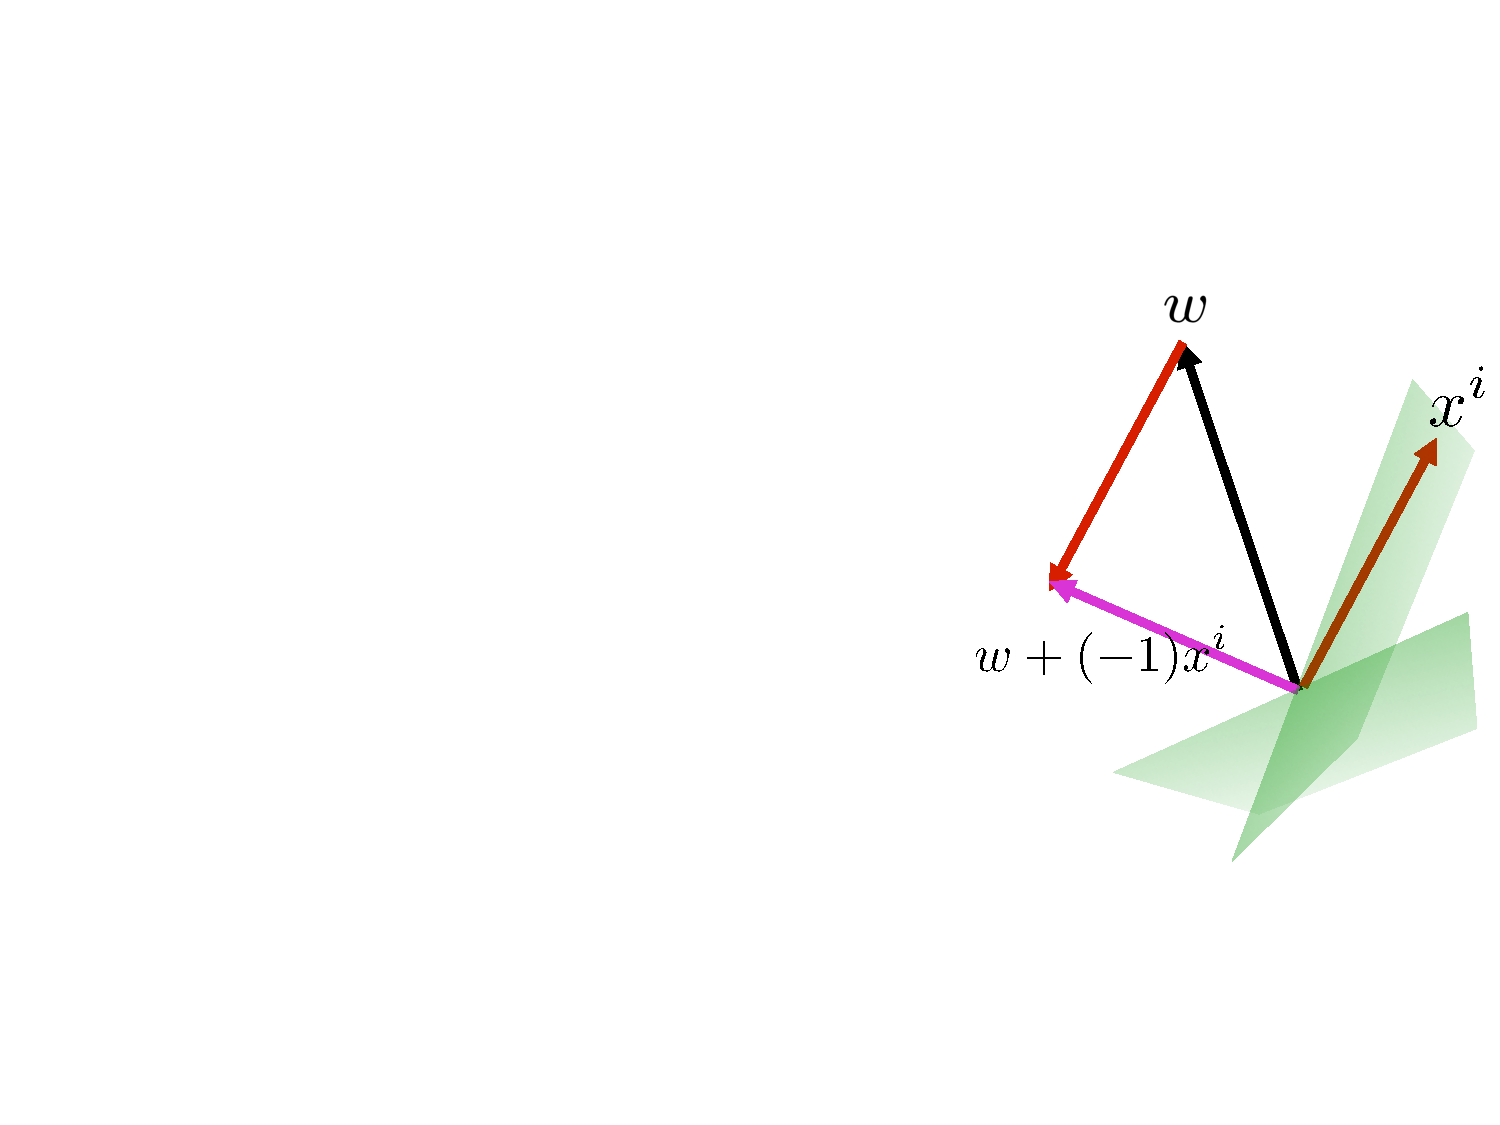
\includegraphics[width=1.0in]{figures/binary_perceptron_rule.pdf}  \hfill \\
 The -1 is the $y^i$ in the equation above.   \hfill \\
   \hfill \\
  
 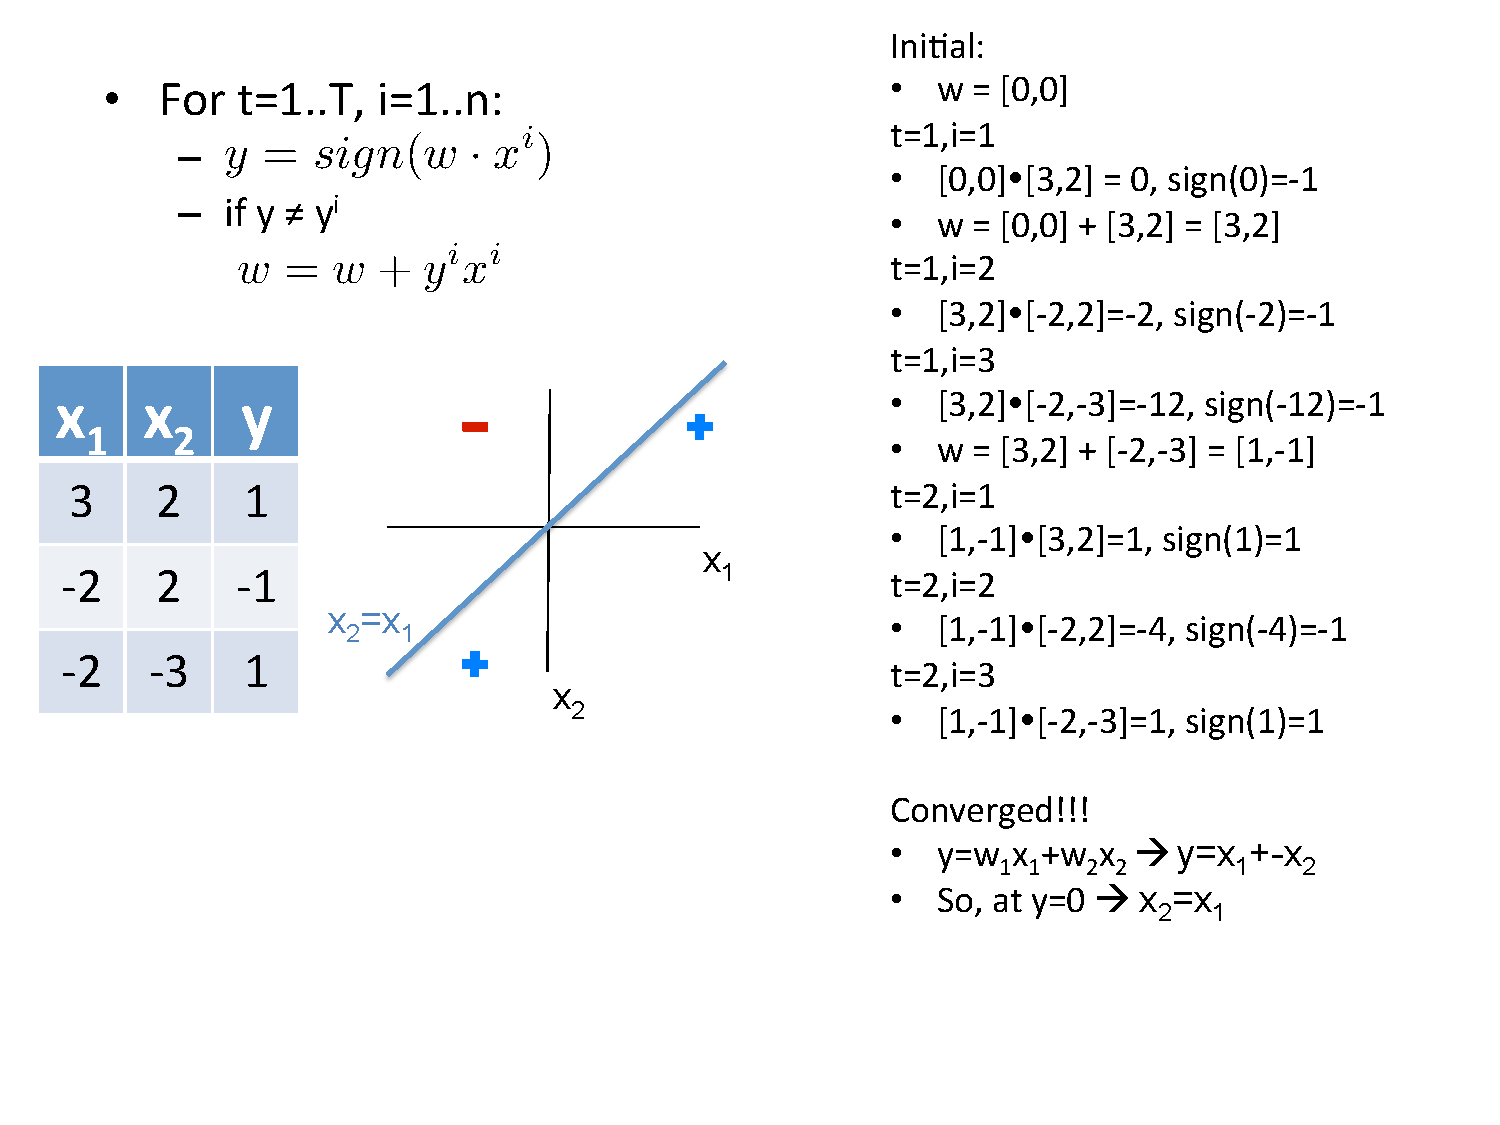
\includegraphics[width=3.2in]{figures/perceptron_chugging_example.pdf}
 
 \underline{$w \cdot x$ and the boundary between positive and negative answers} \hfill \\
If a point has w * x = 1000, a small change in x might change w * x' to 999, or 1001, but it surely won't make w * x a negative value. On the other hand, if w * x = 0.0001, even tiny changes to x might make w * x' negative. And by extension, cases where w * x = 0 where even the tiniest change might make w * x' change sign. So the values where w * x = 0 are those that are on the boundary between positive and negative examples.[1]

So \textbf{the equation w * x = 0 defines the boundary between the positive and negative region}. Now let's unpack that statement. w is a fixed vector, while x is a variable point. So think of w = [w1, w2] as constants, and x = [x1, x2] as variables. The equation w * x = 0 is just another way of writing the equation w1 x1 + w2 x2 = 0. But this is a linear equation in two variables, so it defines a line. You can algebraically solve the equation for x2, and that gives you the "standard form" of the equation of a line, which you can then draw.

[1] The boundary of a region is defined as the set of points where even points very close by can be outside that region.

 
 \subsection{Multiclass Decision Rule}
 
 If we have more than two classes: 
 \begin{itemize}
 	\item we have a weight vector for \textbf{each} class: $w_y$
	\item we calculate an activation for each class: \hfill \\
		activation$_w(x,y) = w_x \cdot x$
	\item the highest activation wins:  \hfill \\
		$y^* = \argmax_y(activation_w(x,y))$ \hfill \\
		"win the vote" 
 \end{itemize}
 
For each point, look at all 3 classes and see which is farthest from the hyperplane.
You can treat the dot product (+ bias) as a confidence from the hyperplane you are.  % week 6 audio. 
\hfill \\ 
\hfill \\
 
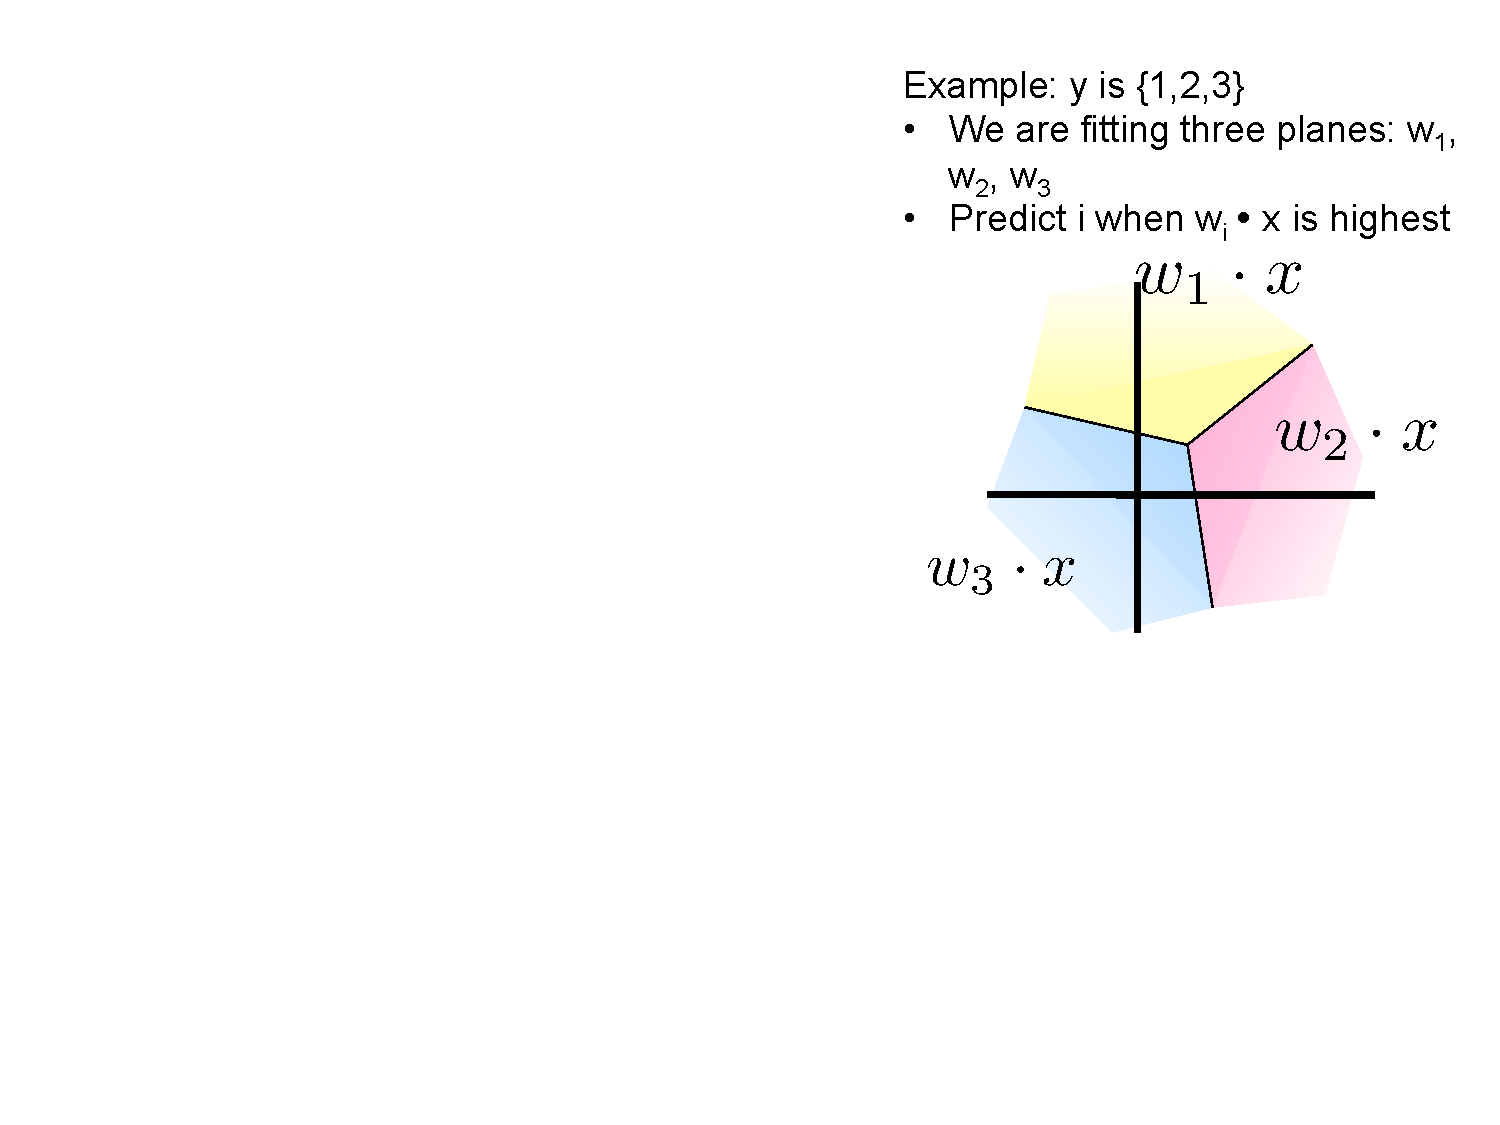
\includegraphics[width=1.5in]{figures/multiclass_decision_rule_planes.pdf}
 
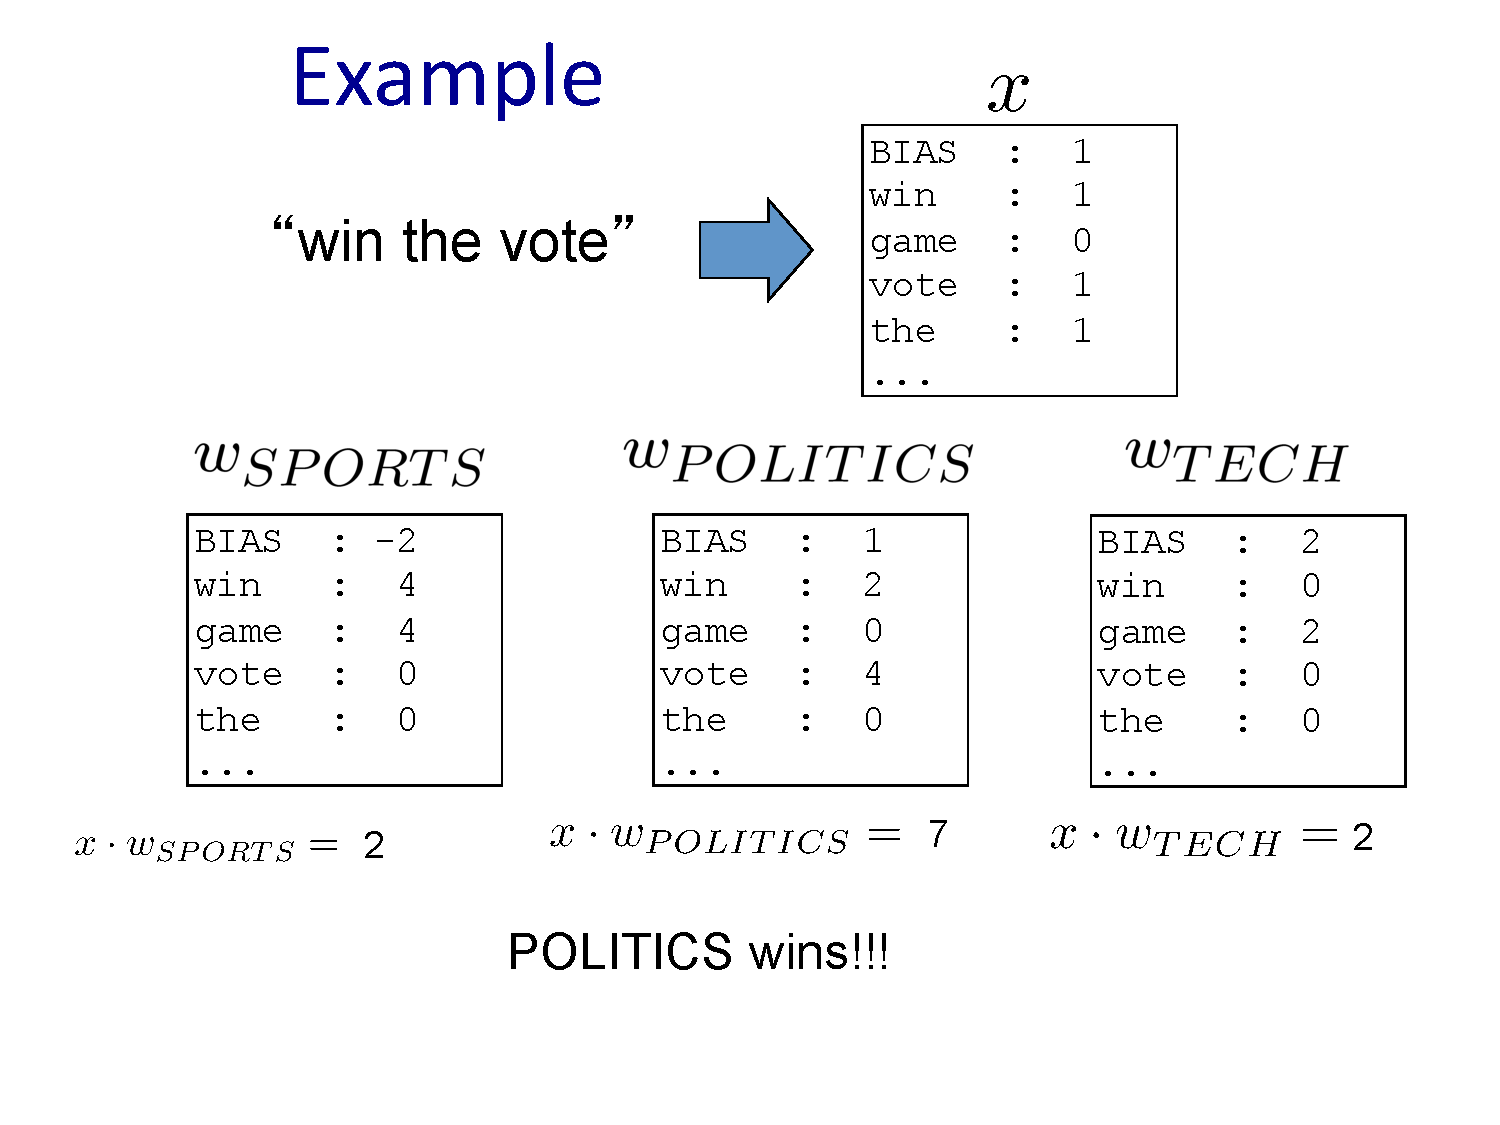
\includegraphics[width=2.5in]{figures/perceptron_multiclass--win_the_vote.pdf}

 \subsubsection{Binary Perceptron Algorithm}
 \begin{itemize}
 	\item start with zero weights: $w_y=0$
	\item for $ t = 1 \dots T$ (T passes over the data):
		\begin{itemize}
			\item for $i = 1 \dots n$ (each training example)
			\begin{itemize}
				\item  Classify with current weights: \hfill \\
					(no more $ y = sign(w_y \cdot x^i)$) \hfill \\
					instead:  $y= \argmax_y w_y \cdot x^i$ \hfill \\
				\item if correct (i.e. $y = y^i$), don't change weights.
				\item if it was wrong, update two vectors: \hfill \\
					$w_{y^i} = w_{y^i} + x^i$ \hfill \\
					If class 2 was the right label, add $x_i$ to $w_2$. \hfill \\
					Also want to push down the wrong classification:  \hfill \\
					(Didn't have to push one down for binary because adding to one pushed the other. )
					$w_y = w_y -x^i$ \hfill \\
			\end{itemize}
		\end{itemize}
 \end{itemize}
 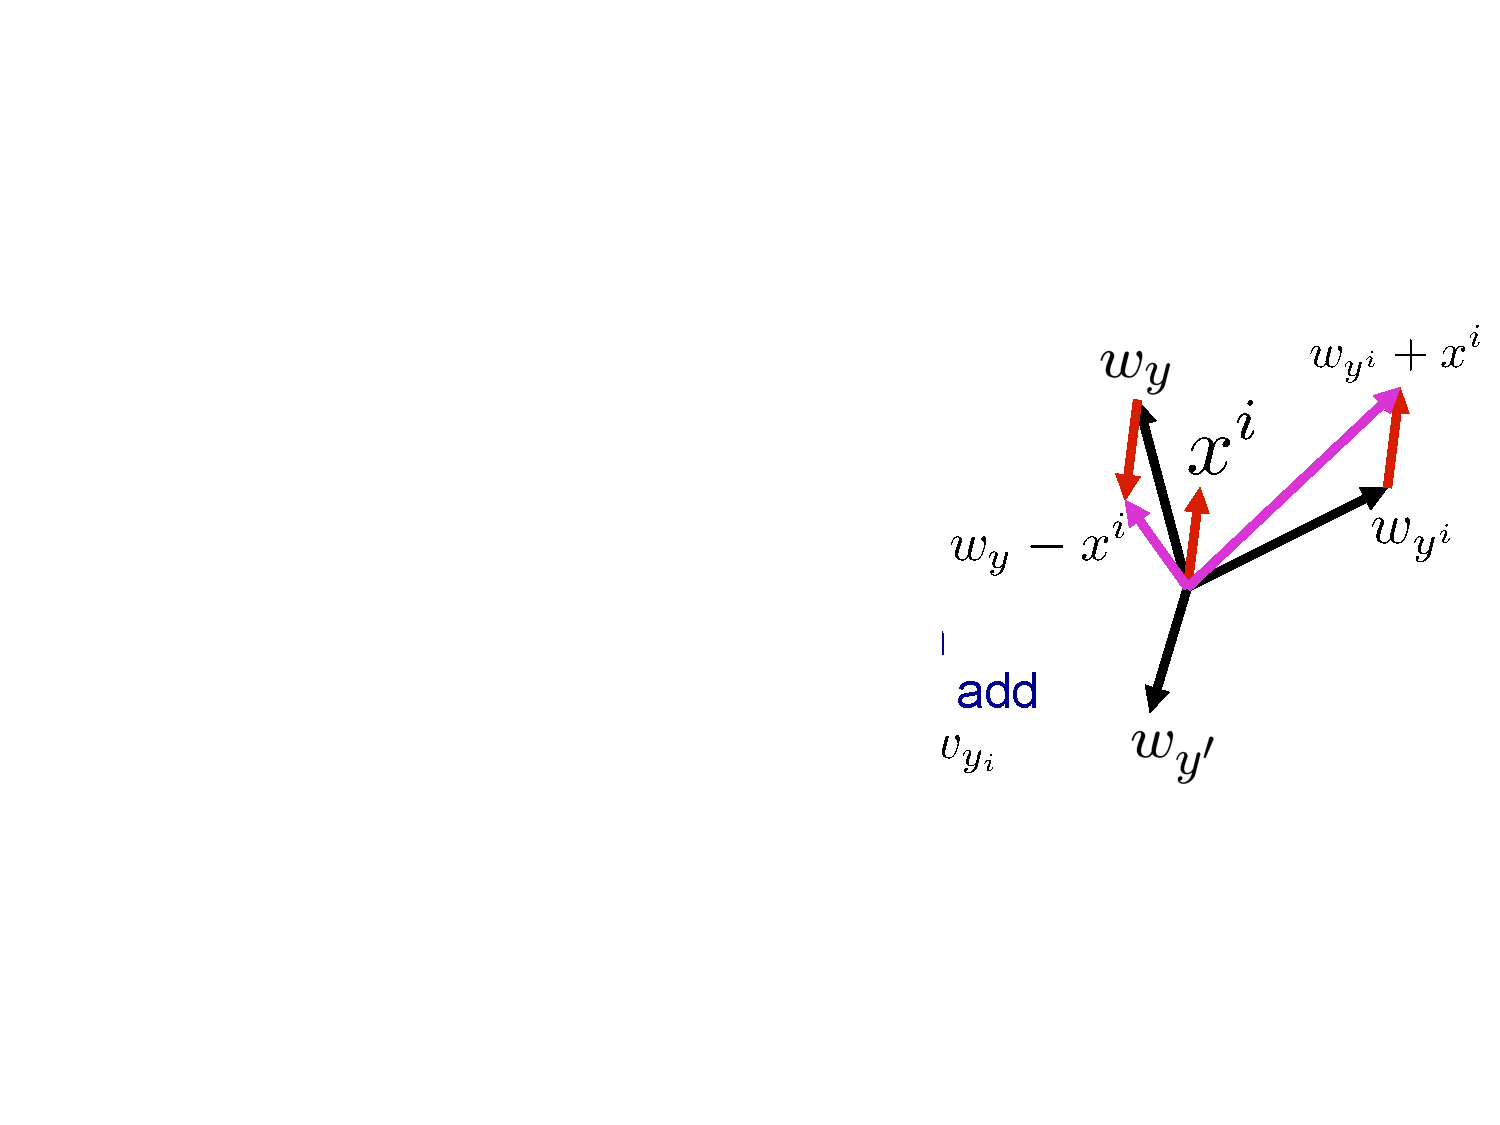
\includegraphics[width=1.0in]{figures/multi_perceptron_rule.pdf}
 
 \subsection{Linear Separability}
 \subsubsection{binary case}
Recall $ \displaystyle  ||x||_2 = \sqrt{\sum_i x_i^2}$ 
 
 The data is linearly separable with margin $\gamma$ if:   \hfill \\
$\exists .w \forall t . y^t (w \cdot x^t) \geq \gamma > 0$.  \hfill \\
Plain english: the data is linearly separable if there exists a w that has a margin greater than zero for all points $t$.  \hfill \\
Note: for $y^t = 1$, $w \cdot x^t \geq \gamma$ and for $y^t = -1$, $w \cdot x^t \leq -\gamma$.  \hfill \\
Plain english: points having label = 1 have a dot product that is greater than $\gamma$, and points that have label = -1 have a dot product that is more negative than $-\gamma$.  \hfill \\
 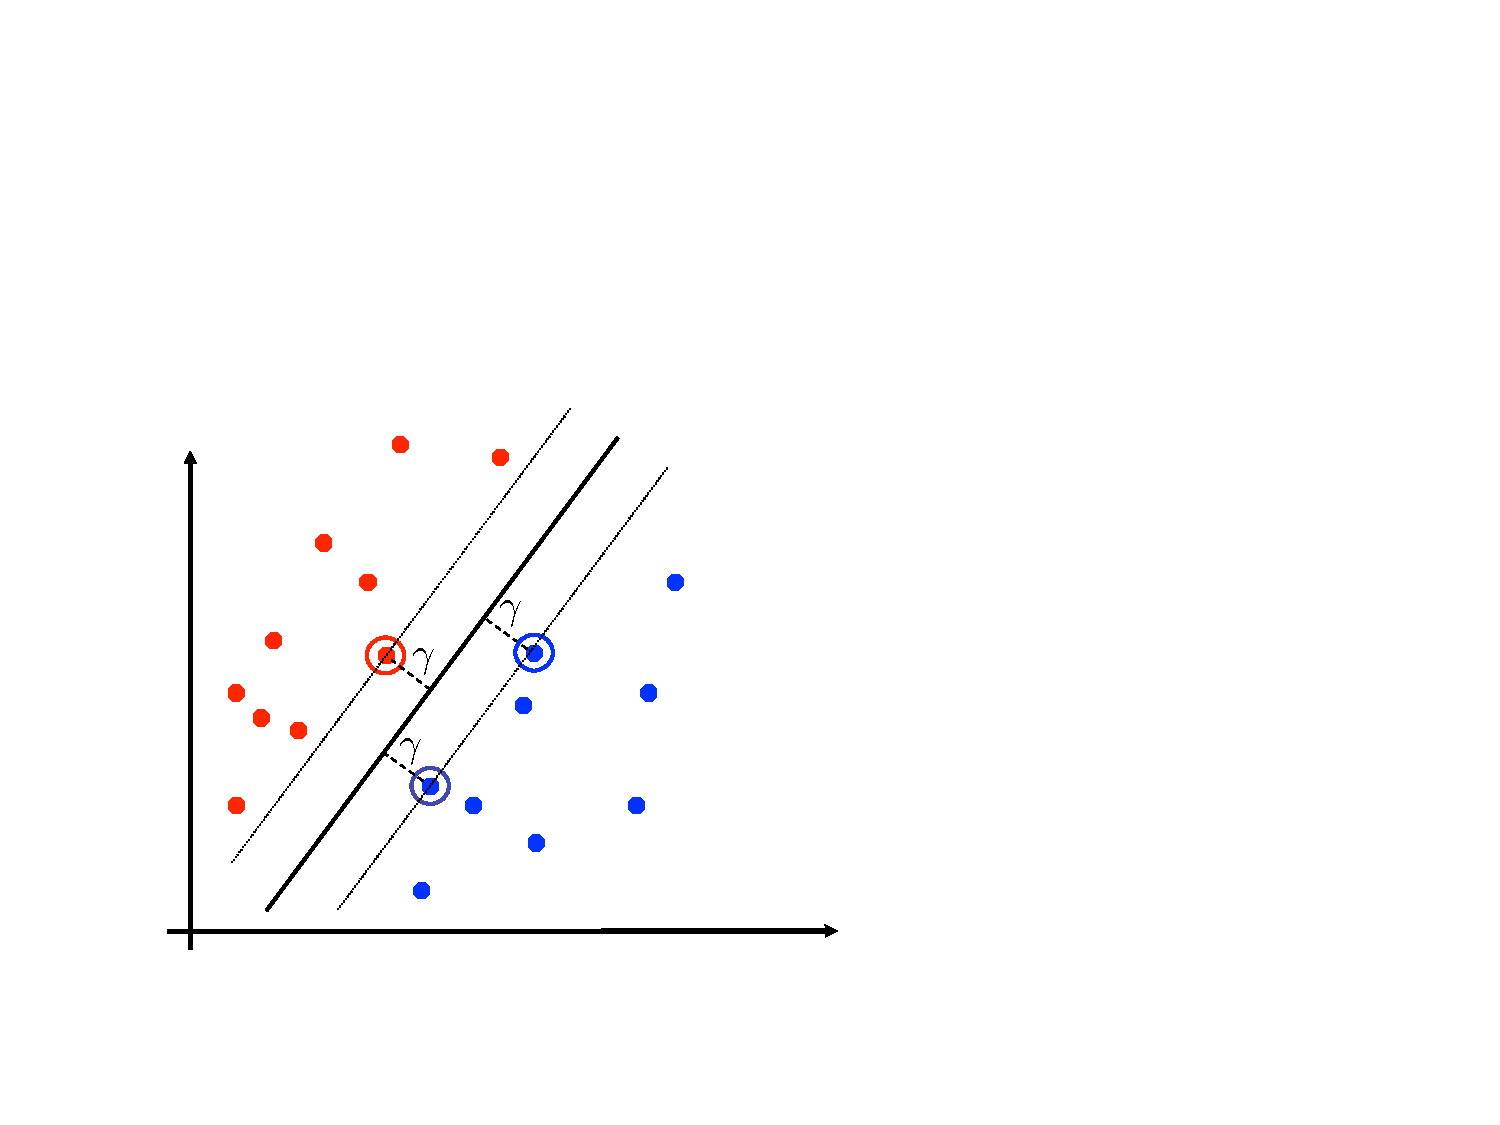
\includegraphics[width=1.0in]{figures/lin_sep_margin.pdf}
 
 \subsubsection{maximum number of mistakes for training linearly separable binary data}
Here, assume the data is separable with margin $\gamma$ and the weight vector is a unit vector: \hfill \\
In math notation, this is: $\exists w^*$ such that $||w^*||_2 = 1$ and $\forall t. y^t(w^* \cdot x^t) \geq \gamma$.) \hfill \\
Recall that you can scale your $w$ (weight) vector(s) by any constant because all you care about is sign($w \cdot x$),
but that this scales your $\gamma$.  You are just multiplying the equation above by a constant.  \hfill \\

Also assume some maximum radius R for your data points:  
$\forall t. ||x^t||_2 \leq R$ \hfill \\
Then the number of mistakes (parameter updates) made by the perceptron is bounded by 
$\displaystyle mistakes \leq \frac{R^2}{\gamma^2}$. \hfill \\
For full inductive proof, see slides.  
Strategy: let $w^k$ be the weights after the k-th update (mistake).  
Then $k^2 \gamma^2 \leq ||w^k||_2^2 \leq k R^2$ \hfill \\
Therefore $k \leq \frac{R^2}{\gamma^2}$.  \hfill \\
\textbf{If there is a linear separator, the Perceptron will find it!} \hfill \\
 \hfill \\
 
The \# of mistakes you need to make for a perceptron to converge is bounded by a ratio of $R/\gamma^2$. \hfill \\
 \hfill \\

What if gamma is small?
    Starting to violate linearly separability rule. 
    Shouldn't trust perceptron under this. 


\subsection{Logistic Regression \& Perceptron similarities}
\underline{Logistic regression}:  \hfill \\
In vector notation, y is in the set $\{ 0, 1\}$. \hfill \\
$w = w + \nu \sum_j [y^j - P(y^j | x^j, w))] x^j$ \hfill \\

\underline{Perceptron}:  \hfill \\
When y is in $\{ 0, 1\}$: \hfill \\
$w = w + [y^j - sign^0(w \cdot x^j)] x^j$  \hfill \\
Note: sign$^0(z) =  + 1$ if $z > 0$ and 0 otherwise.  \hfill \\
\hfill \\
Differences:   \hfill \\
1. Online vs. batch learning.  Logistic regression is batch, Perceptron is on-line.  \hfill \\
2. Logistic is probabilistic and Perceptron is error-driven. 
 




\section{Support Vector Machines}
\smallskip \hrule height 2pt \smallskip

Vocab: 
\begin{itemize}
	\item $i$ or $j$: the $i^{th}$ or $j^{th}$ data (training) point. 
	\item $\bm{w}$: the weights of the model.  The black line is perpendicular to this vector. 
	\item $\bm{w} \cdot \bm{x}$: the distance from x to the decision boundary. 
	\item $\bm{w} \cdot \bm{x} + w_0$: to move the decision boundary off the origin, you need to shift it by a constant.  
	\item $\bm{w}_0$: a constant that defines a line parallel to the decision boundary and is $w_0$ units away. 
\end{itemize}

Like perceptron, but maximizes the margin.  

Optimizing a small weight vector: $\displaystyle min_w \: \frac{1}{2}||w||^2$ \hfill  \\  % \: gives 4/18ths of \quad space.
	% https://www.andy-roberts.net/res/writing/latex/hspacing.pdf
and getting points right: $\forall \mbox { points } i, y$  $w_{y^*} \cdot x^i \geq w_y \cdot x^i + 1$
Summary:
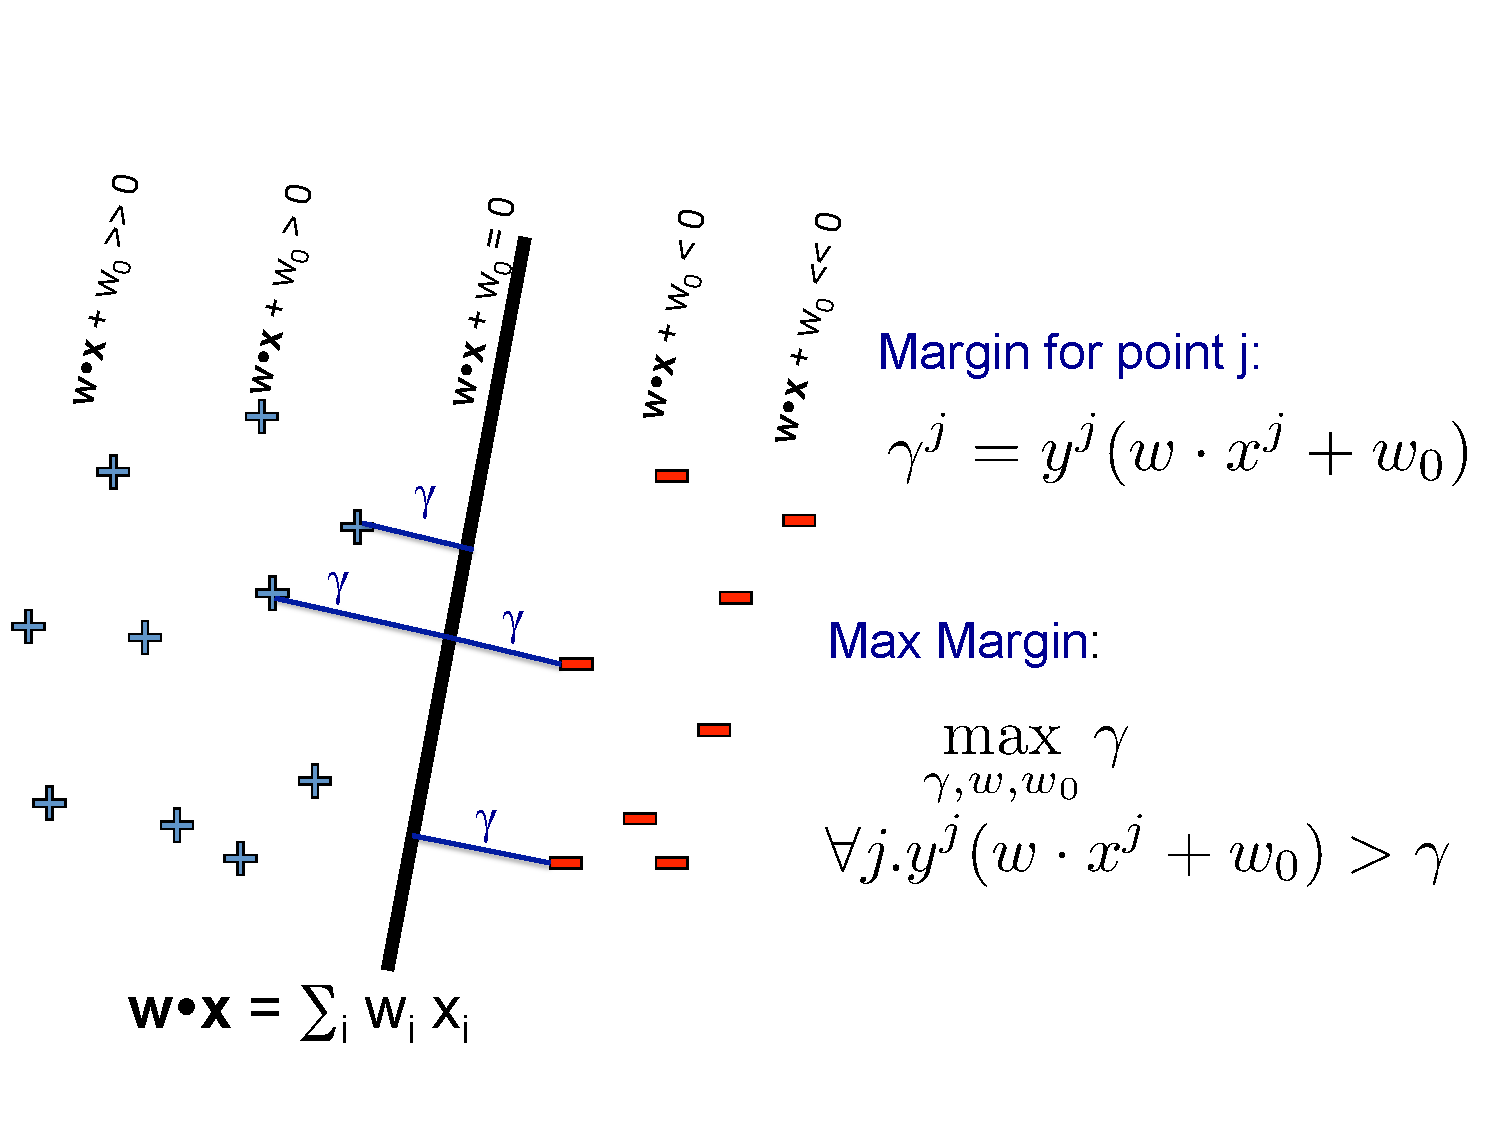
\includegraphics[width=2.5in]{figures/svm_overview.pdf}

There are many possible ways to write the same line: \hfill \\
If $\bm{w} \cdot \bm{x} + w_0 = 0$, then these also work: 
$2\bm{w} \cdot \bm{x} + 2w_0 = 0$, $1000\bm{w} \cdot \bm{x} + 1000w_0 = 0$, $\dots$ \hfill \\
Any constant scaling has the same intersection with the z = 0 plane, so you get the same dividing line. \hfill \\
\textbf{This is why we \underline{don't} want} max$_{\gamma, w, w_0}$. \hfill \\  \hfill \\

%Recall that the distance from the the decision boundary to a point is given by $\gamma$
%\includegraphics[width=2.5in]{figures/svm_dist_to_plane.pdf}

The distance from $x^j$ to the decision boundary is given by $\lambda \frac{w}{||w||_2}$ :  \hfill \\
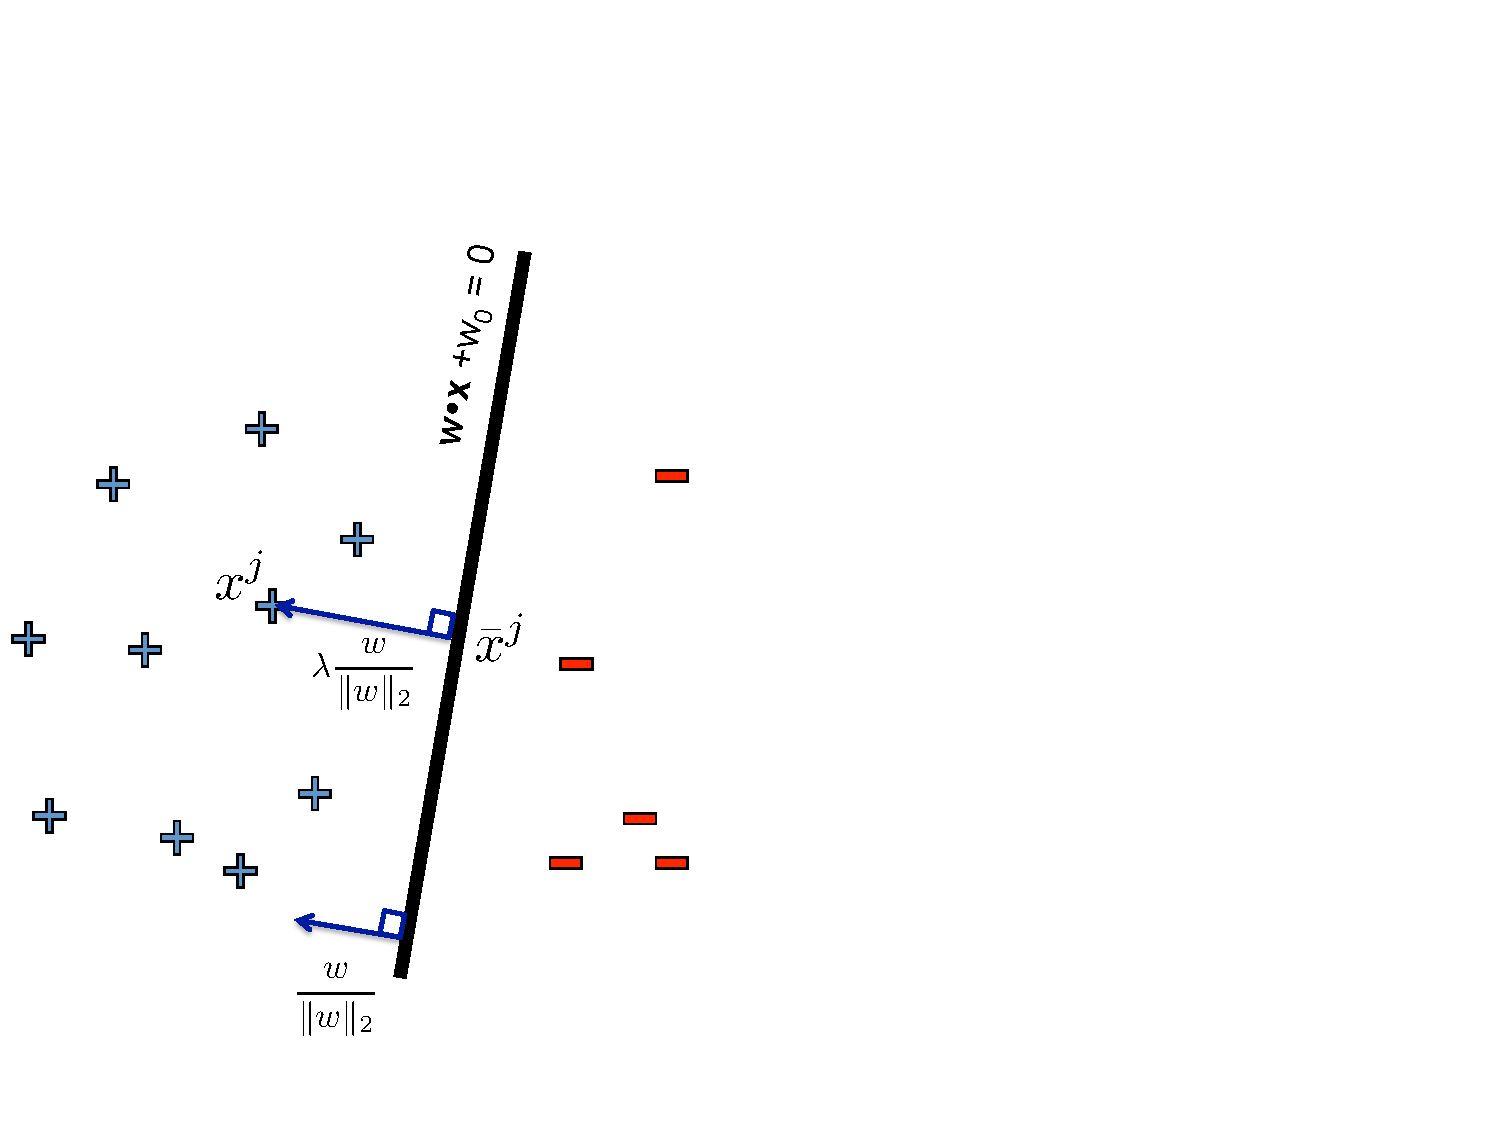
\includegraphics[width=1.5in]{figures/svm_component_norm_to_decision_boundary.pdf}  \hfill \\
$\bar{x}^j$ is the component of $x^j$ that is normal to $w$. \hfill \\
So $x^j = \bar{x}^j + \lambda \frac{w}{||w||_2}$  \hfill \\
(Recall $||w||_2 = \sqrt{\sum_i w_i^2}$)  \hfill \\   \hfill \\

\subsection{motivation for minimizing the norm of the weights}
We can maximize the margin by minimizing $||w||_2$: 
$\gamma = \frac{||w||_2}{w \cdot w} = \frac{1}{||w||_2}$   \hfill \\
Derivation:  \hfill \\
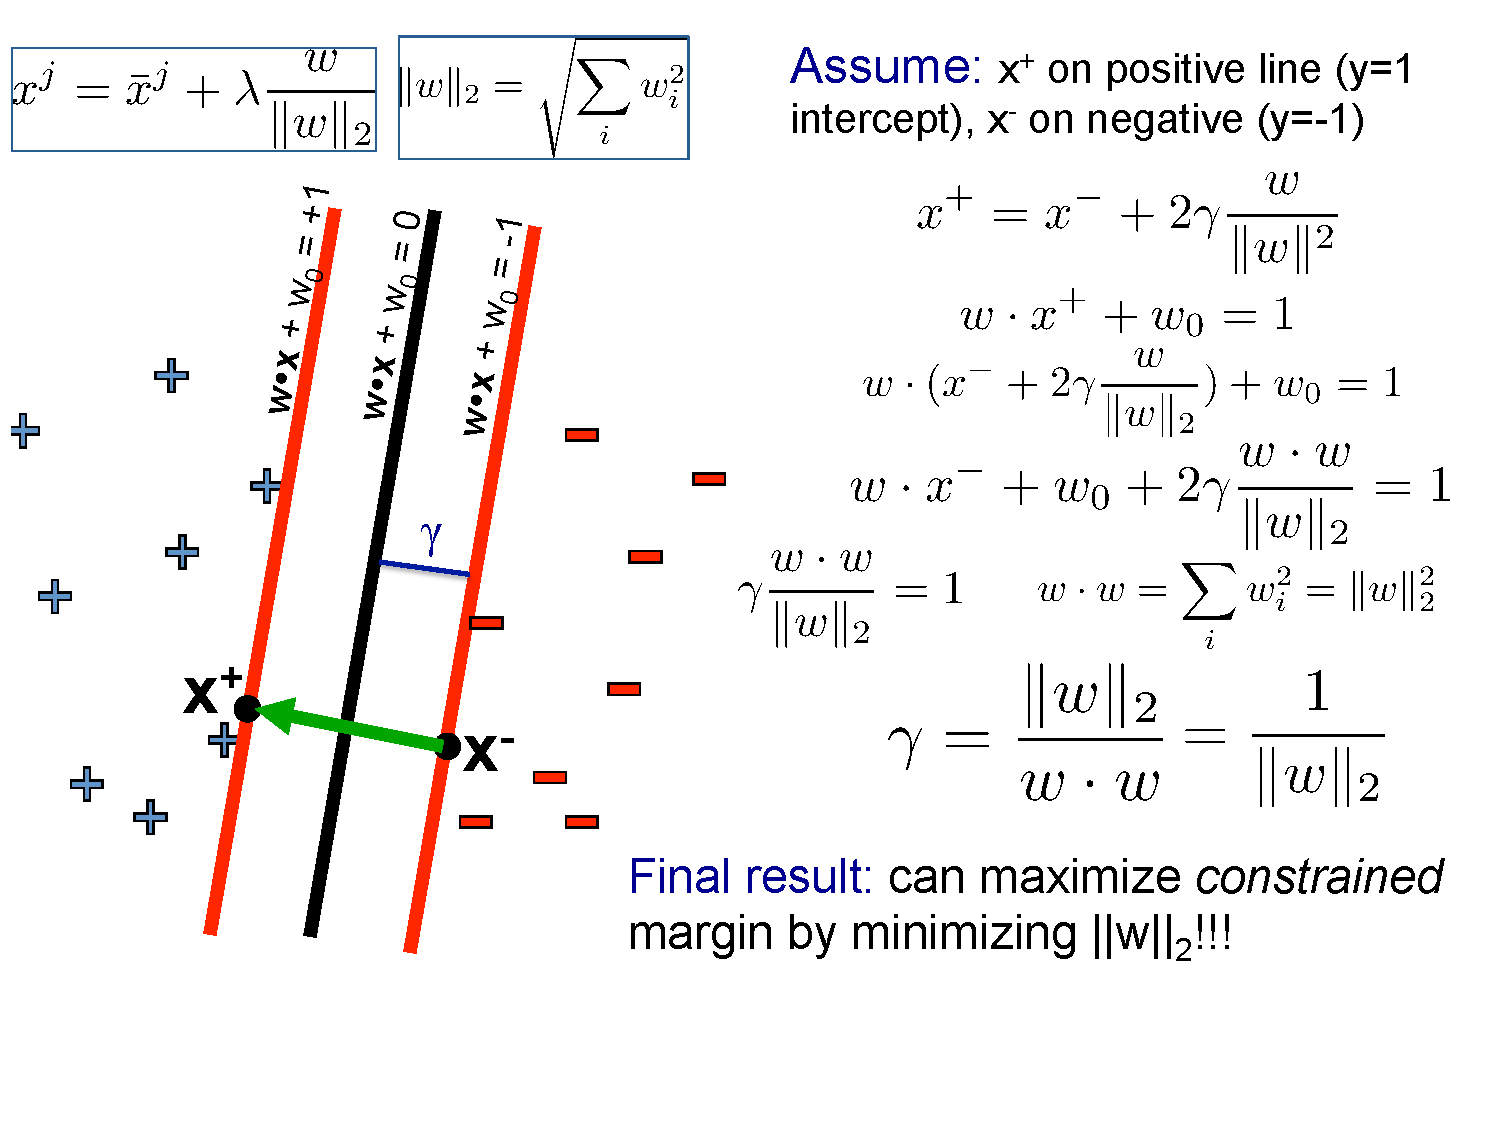
\includegraphics[width=2.7in]{figures/svm_derivation_of_minimizing_weights.pdf} \hfill \\

Intuitive explanation, after 2 key facts:  \hfill \\
\begin{itemize}
	\item Key fact \#1: the bigger your $\bm{w}$ is, the \underline{closer} the line $\bm{w}\bm{x}=1$ is to the line $\bm{w}\bm{x} = 0$.  		Small distance between $\bm{w}\bm{x}=1$ and $\bm{w}\bm{x}=0$ translates to a small margin.  
		Note that you could use any constant in place of 1. 
	\item Key fact \#2: The $w_0$ just shifts the black decision boundary line away from the origin.  
\end{itemize}
Now we can explain why minimizing the norm of the weights leads to the largest margin. 

\begin{itemize}
	\item Imagine $w_0 = 0$, meaning the decision boundary goes through the origin.  \hfill \\
	\item Now let $w = [2, 0]$ for simplicity.    
		Where is the decision boundary?  
		The decision boundary corresponds to $2 x_0 + 0 x_1 = 0$.  
		That means the decision boundary is along $x_0 = 0$, which is a line through the $x_1$ (vertical) axis. 
	\item But the point is that when you set $\bm{w} \cdot \bm{x} = c$ or some other constant.
		Key fact \#1 says that the larger w is, the farther $\bm{w} \cdot \bm{x} = 0$ is from $\bm{w} \cdot \bm{x} = c$  
		In this case where $w_1 = 0$, you have  $w_0 x_0 = c$, or $x_0 = c/w_0 = c/2$.  
		If you want the $=1$ line far from the decision boundary, you need to increase the distance between these lines.
		Since $c$ is fixed, so the only way we can do this is to decrease $w_0$. 
	\item The logic holds true for when $w_1$ is nonzero: you just want to minimize the size of the $\bm{w}$ vector.
		Minimizing the size of $w$ is equivalent to minimizing $||w||_2$ 
\end{itemize}

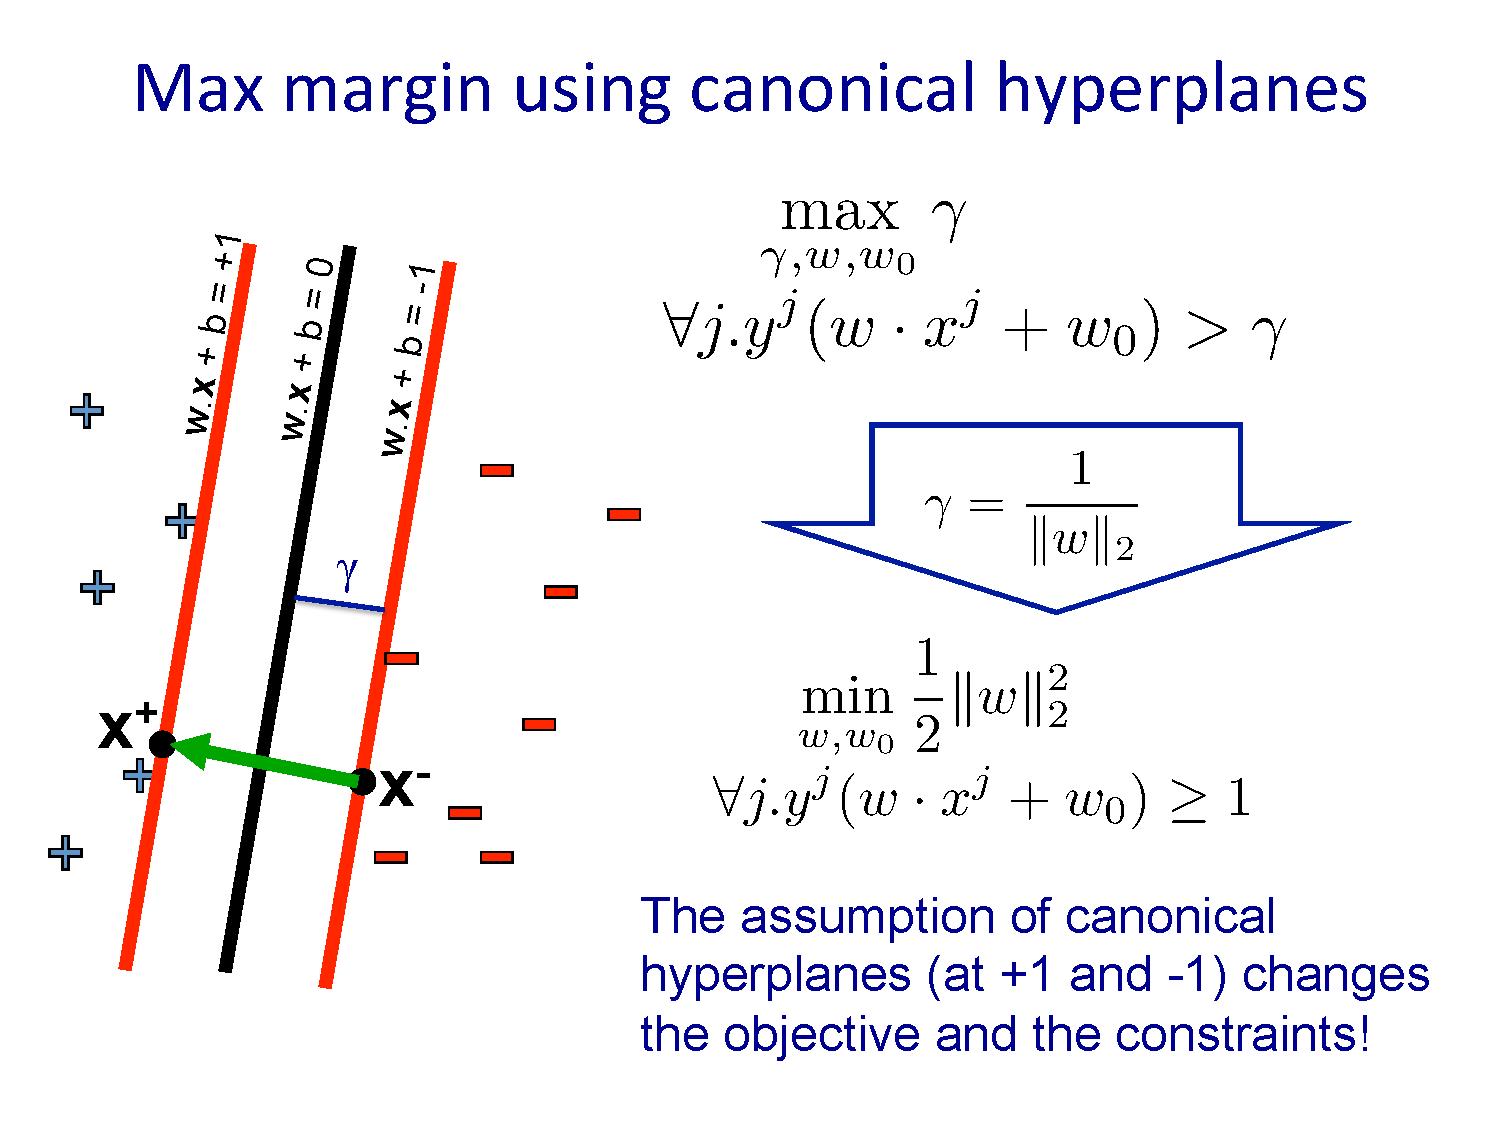
\includegraphics[width=2.7in]{figures/max_margin_using_canonical_hyperplanes.pdf}

\subsection{SVM recipe}
We want to minimize the norm subject to getting the predictions right:  \hfill \\
$\displaystyle  \min_{w, w_0} \frac{1}{2} ||w||_2^2$ so that $\forall j . y^j(w \cdot x^j + w_0) \geq 1$

We do this with quadratic programming (QP). 
The decision boundary is defined by \textbf{support vectors}, which are data points on the canonical red lines. 
All the points that aren't on the red line are non-support vectors. \hfill \\
 \hfill \\
 If your data is not linearly separable, you can add nonlinear features.
 These are called Kernels, and will be discussed later. 
 
 \subsection{Balancing \# of mistakes and $||w||_2^2$}
 If your data isn't linearly separable, then you might need to allow your $||w||_2$ to be a little bigger and make a few mistakes. 
One option: 
 $\displaystyle  \min_{w, w_0} \frac{1}{2} ||w||_2^2 + M$ (M = \# of mistakes)  \hfill \\
 so that $\forall j . y^j(w \cdot x^j + w_0) \geq 1$
 
 \subsubsection{Hinge Loss}
 One way to balance the number of mistakes and how big $w$ is:  
  $\displaystyle  \min_{w, w_0} \frac{1}{2} ||w||_2^2 + C \sum_j \xi^j$ \hfill \\
 so that $\forall j . y^j(w \cdot x^j + w_0) \geq 1 - \xi^j$ \hfill \\
 C = strength of penalty. \hfill \\
 $\xi$ is size of error for each error.  If the point is classified correctly, $\xi$ is zero.   \hfill \\
 When we want the dot product \& shift $\geq 1 - \xi^j$, the 1 is for the green-line margin, and you are wrong by $\xi$  amount. \hfill \\
 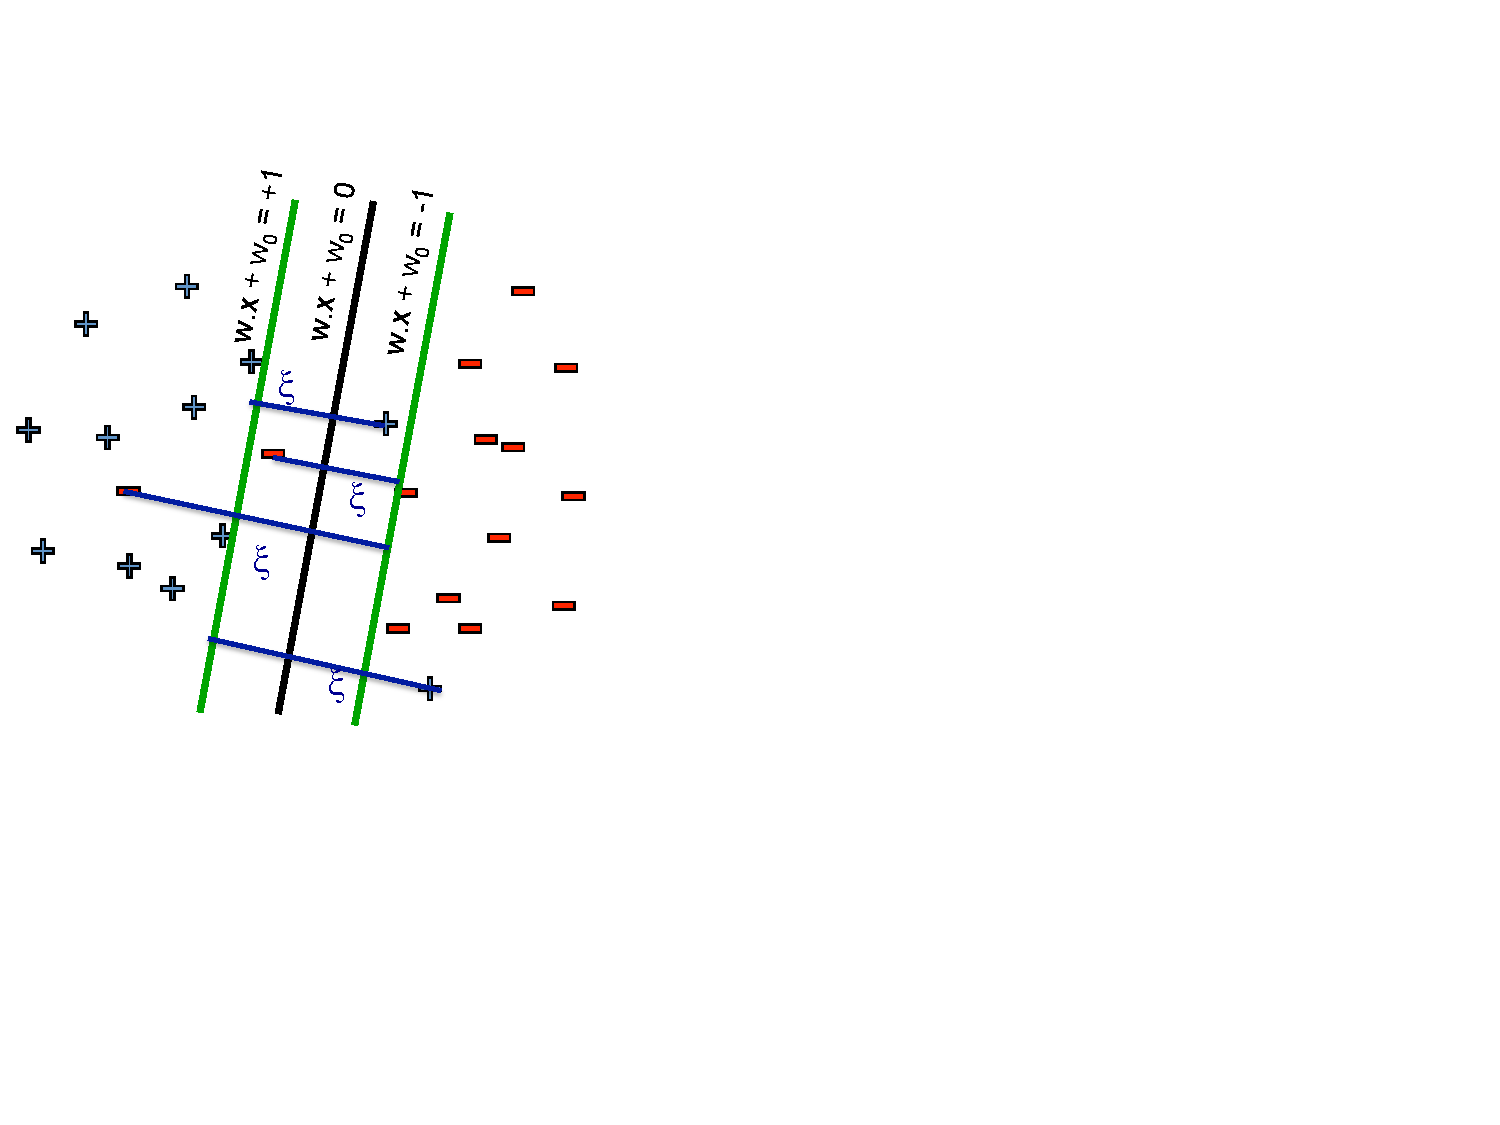
\includegraphics[width=1.5in]{figures/hinge_loss_xis.pdf}
 \hfill \\
 Now we can tune our balance between asking for small weights $\bm{w}$ and asking for perfect classification. 
 \begin{itemize} 
 	\item $C  = \infty \rightarrow$ pressure to separate the data, even if the margin is skinny.
	\item $C = 0 \rightarrow$ fat margins over accuracy. 
\end{itemize}
Use your training set to train C.  \hfill \\ 
Note that if \_\_\_\_\_ $\geq 1$, you don't care if the point is classified wrong.   % had used "margin" but this doesn't make sense!
But if \_\_\_\_\_ $ < 1$, you pay a linear penalty. % had used "margin" but this doesn't make sense! 
\hfill \\

\textbf{Hinge Loss:}  \hfill \\
$\displaystyle \min_{w, w_0} \frac{1}{2} ||w||_2^2 + C \sum_{j=1}^N [1 - y^j(w \cdot x^j + w_0)]$ \hfill \\
$1^{st}$ term is regularization, $2^{nd}$ term is hinge loss.  \hfill \\
Solve by differentiating and set equal to zero.  \hfill \\
There is no closed form solution, but quadratic program is concave.  (??)   \hfill \\
Hinge loss is not differentiable (??), so gradient ascent is a little trickier.  \hfill \\

\subsubsection{Logistic Regression to Minimize Loss}
Logistic regression assumes $P(Y=1 | X=x) = \frac{exp(f(x))}{1 + exp(f(x))}$  \hfill \\
(For Logistic Regression, $f(x)$ was $w_0 + \sum_i w_i X_i$ and we had $Y = \{0, 1\}$)  \hfill \\
Now we have $Y = \{ -1, +1 \}$.  \hfill \\
To maximize data likelihood for $Y = \{ -1, +1 \}$: \hfill \\
$\displaystyle  P(y^i | x^i) = \frac{1}{1 + exp(-y^i f(x^i))}$ \hfill \\
\begin{align*}
	\ln P(D_Y | D_{\bm{X}}, \bm{w}) &= \sum_{j=1}^N \ln P(y^j | x^j, w) \\ 
		& \mbox{plug in the $P$ above} \\
		&= - \sum_{i=1}^N \ln(1 + exp(-y^i f(x^i)))
\end{align*}
Since $-\ln(z) = \ln(1/z)$ we get to minimize this (negative):   \hfill \\
$\displaystyle  \sum_{i=1}^N \ln(1 + exp(-y^i f(x^i))) =  \sum_{i=1}^N \ln(1 + exp(-y^i [w_0 + \sum w_i x_i]))$

\subsubsection{SVMs vs Regularized Logistic Regression}
\textbf{SVM Objective:} \hfill \\
$\displaystyle \argmin_{\bm{w}, w_0} \frac{1}{2} ||w||_2^2 + C \sum_{j=1}^N [1 - y^j f(x^j)]_+$ \hfill \\
where $[x]_+ = max(x , 0)$ \hfill \\
 \hfill \\

\textbf{Logistic Regression Objective:} \hfill \\
$\displaystyle  \argmin_{\bm{w}, w_0} \lambda ||w||_2^2 + \sum_{j=1}^N ln(1 + \exp(-y^j f(x^j)))$ \hfill \\
 \hfill \\
 
 Note that SVM and Logistic Regression have the same $l_2$ regularization term, but different error terms. 

 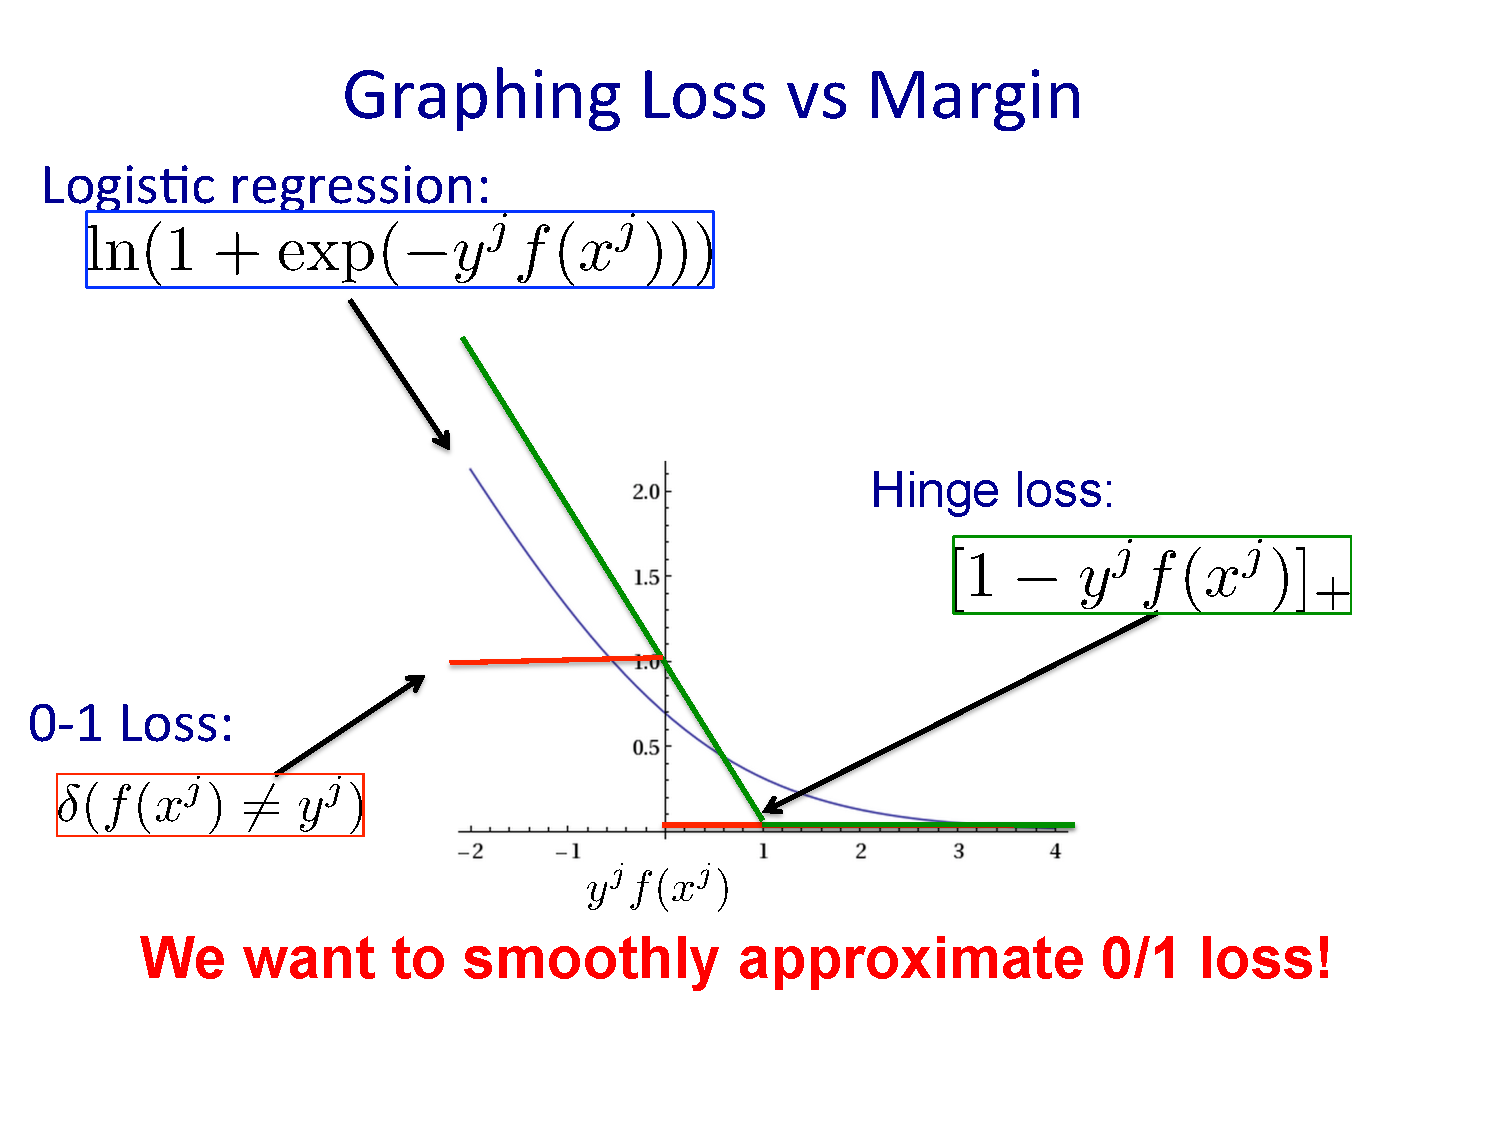
\includegraphics[width=2.5in]{figures/LR_svm_step_losses.pdf}
 
 \subsection{Multi-class SVMs}
 To do 3 classes, you need to learn 3 classifiers. \hfill \\
 Can't just do $y = \argmax_i w_i \cdot x$ for $i$ classifiers.  
 Wouldn't handle this: 
 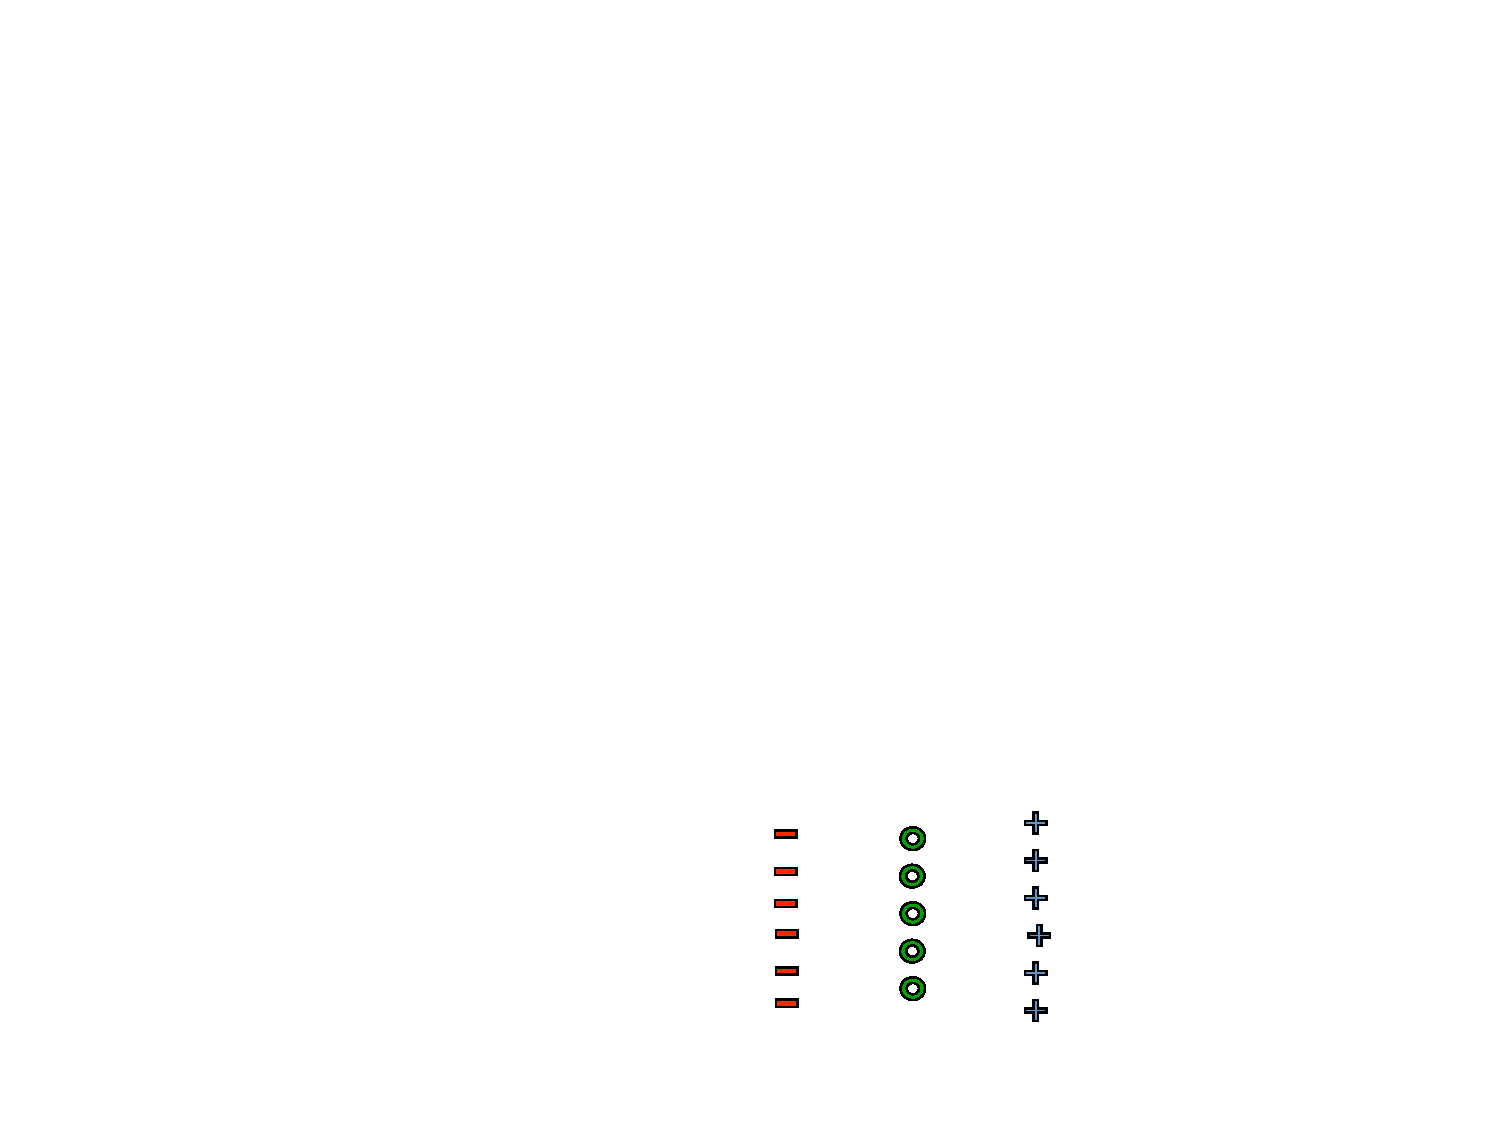
\includegraphics[width=0.6in]{figures/multiclass_svm_motivation.pdf}
 \hfill \\  \hfill \\
 
 Instead, we learn 3 classifiers for these 3 symbols: 
 \begin{enumerate}
 	\item + vs $\{ O, - \}$, weights $w_+$
	\item + vs $\{ O, + \}$, weights $w_-$
	\item + vs $\{ +, - \}$, weights $w_O$
 \end{enumerate}
 But to get it working for that set of 3 columns, we need additional constraints.  \hfill \\
 For each class: \hfill \\
 for class $y'$ that is not class $y^j$ ($\forall y' \neq y^j$):  \hfill \\
 And for all classes $j$ ($\forall j$):  \hfill \\
 $w^{y^j} \cdot x^j + w_0^{y^j} \geq w^{y'} \cdot x^j + w_o^{y'} + 1$. \hfill \\
 ($\forall$ = "for all") \hfill \\
 In plain english: ????.   \hfill \\
 ??? Do I have the fact that j is for classes right?  (Could j still be points?)  ??
 \hfill \\
 \hfill \\
 
We can also introduce slack variables as before. 
$\displaystyle \min_{w, w_0} \sum_y ||w^y||_2^2 + C \sum_j \xi^j$ \hfill \\
$w^{y^j} \cdot x^j + w_0^{y^j} \geq w^{y'} \cdot x^j + w_o^{y'} + 1 - \xi^j$. \hfill \\
That's true for class $y'$ that is not class $y^j$ ($\forall y' \neq y^j$), and all classes $j$ ($\forall j$) and for all $\xi^j > 0$ \hfill \\
 \hfill \\
 
 So you can do multiple classes in a one against all approach *or* a multiclass SVM approach.  
 

 
  





\section{Kernels}
\smallskip \hrule height 2pt \smallskip
If the data is not linearly separable and/or you want a wiggly boundary, use kernels. 




\section{Ensemble Methods}

\smallskip \hrule height 2pt \smallskip

Vocab
\begin{itemize}
	\item \textbf{decision tree stump}: 
	\item \textbf{decision stub}:  (used in lecture 10 pg 14: boosting)  ?? horizontal or vertical line only?  
	\item \textbf{axis aligned classifier}
\end{itemize}

Instead of learning a single classifier, learn many weak classifiers that are good at different parts of the data. 
The output class is a weighted vote of each classifier. 
\begin{itemize}
	\item classifiers that are most "sure" will vote with more conviction
	\item classifiers will be most "sure" about a particular part of the space. 
	\item on average, these will do better than a single classifier. 
\end{itemize}

% transcribed understanding of audio from week 8
This is better than breaking up the space into a bunch of sub-spaces and making single classifiers for each.  
If you had single classifiers for sub-spaces, you would be losing information about the surroundings.
It is better to have all classifiers cover the whole space, but let them vote. 

\subsection{Bagging vs Boosting}
\textbf{Bagging:} % http://stats.stackexchange.com/questions/18891/bagging-boosting-and-stacking-in-machine-learning
\begin{itemize}
	\item parallel ensemble: each model is built independently
	\item aim to decrease variance, not bias
	\item suitable for high variance low bias models (complex models)
	\item \textbf{samples are drawn with replacement}
	\item each model in the ensemble vote with equal weight % https://en.wikipedia.org/wiki/Ensemble_learning
	\item an example of a tree based method is random forest, which develop fully grown trees (note that RF modifies the grown procedure to reduce the correlation between trees)
\end{itemize}

\textbf{Boosting:}  % http://stats.stackexchange.com/questions/18891/bagging-boosting-and-stacking-in-machine-learning
\begin{itemize}
	%\item sequential ensemble: try to add new models that do well where previous models lack
	\item \textbf{incrementally building an ensemble by training each new model instance to emphasize the training instances that previous models mis-classified.} 
	\item aim to decrease bias, not variance
	\item suitable for low variance high bias models
	\item an example of a tree based method is gradient boosting
	\item In some cases, boosting has been shown to yield better accuracy than bagging, but it also tends to be more likely to over-fit the training data. % https://en.wikipedia.org/wiki/Ensemble_learning
	\item AdaBoost is the most common
\end{itemize}


\subsection{Bagging}
\textbf{"Bagging" = \underline{B}ootstrap \underline{AGG}regation.}
For $i = 1, 2, \dots, K$:   (?? translate to english ??) 
\begin{itemize}
	\item $T_i \leftarrow$ randomly select $M$ training instances with replacement.
	\item $h_i \leftarrow$ learn($T_i$)
\end{itemize}
Then combine the $h_i$ together with uniform voting ($w_i = 1/K$ for all $i$).

\subsubsection{Example: CART decision boundary}
CART is a decision tree learning algorithm. \hfill \\

100 bagged trees:  shades of blue/red indicate the strength of votes for particular classifications. \hfill \\
Picked random subsets of the data, and built classifiers.  These classifiers are weighted!! \hfill \\  % week 8 audio
?? (not the strength of different classifiers.)   \hfill \\ 
?? Is white an overall uncertain vote ??   \hfill \\ 
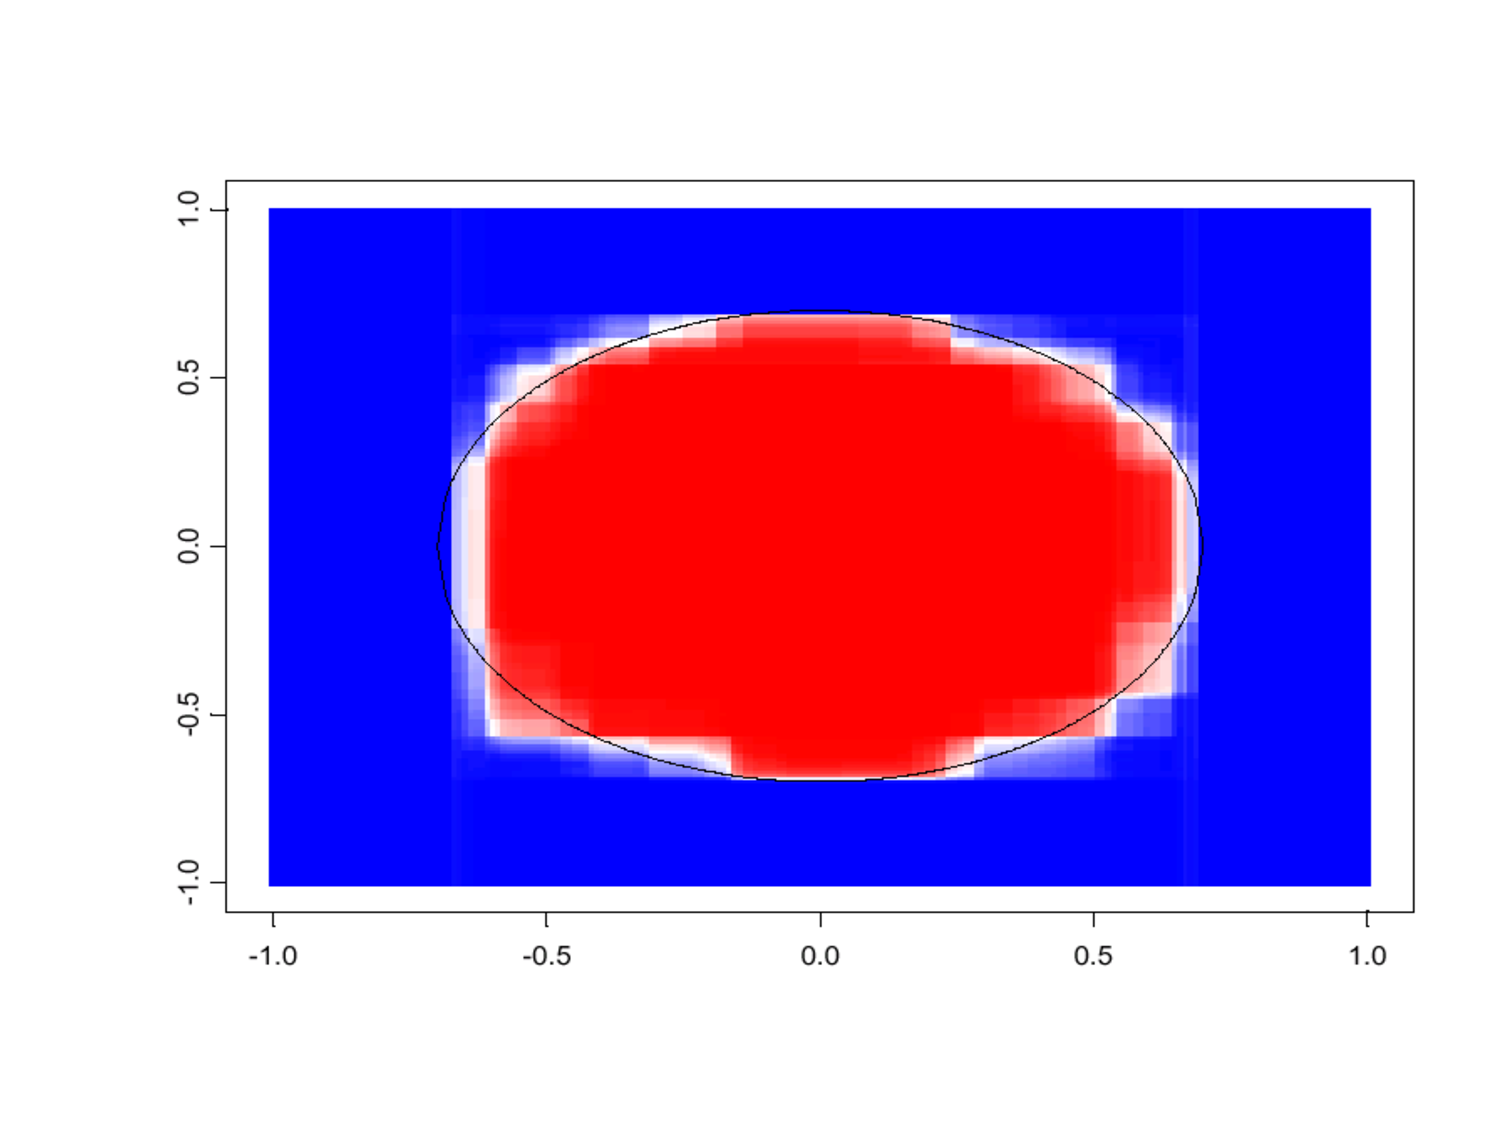
\includegraphics[width=2in]{figures/100_bagged_trees.pdf} \hfill \\
Approximating the circle with a set of lines.  Piecewise linear functions. \hfill \\ % wk 8 audio
The more trees you have, the smoother the boundary will be. 

\subsubsection{Fighting the bias-variance tradeoff}
Simple (a.k.a. weak) learners are good. \hfill \\ 
Examples of weak learners we can use: \hfill \\ 
Naive Bayes, logistic regression, perceptron, decision stumps, shallow decision trees, etc. \hfill \\ 
These learners have low variance; they don't usually overfit. 

But simple (a.k.a. weak) learners are also bad: \hfill \\ 
They have high bias (high error), so you can't solve hard learning problems. \hfill \\ 

The solution: Boosting. 

\subsection{Boosting}

\begin{itemize}
	\item Combine	weak	classifiers	to get very strong classifier.  
		The weak classifiers only have to be slightly better than random on the training data. 
		You end up with a very strong classifier.  You can get zero training error. 
	\item AdaBoost is the most common algorithm
	\item Similar to logistic regression:
		\begin{itemize}
			\item both linear models.  Boosting "learns" features.  
			\item similar loss functions
			\item single optimization (Logistic Regression) versus incrementally improving classification (Boosting) 
		\end{itemize}
	\item  boosting with a weak classifier is better than using a fancy classifier. 
		A boosted version will always do better than the vanilla one. 
	\ 
\end{itemize}


An approach to calculate the output using several different models and then average the result using a weighted average approach. 
By combining the advantages and pitfalls of these approaches by varying your weighting formula you can come up with a good predictive force for a wider range of input data, using different narrowly tuned models.  % http://stats.stackexchange.com/questions/18891/bagging-boosting-and-stacking-in-machine-learning

Boosting is ensemble method. \hfill \\
\underline{The idea}: given a weak learner, run it multiple times on (reweighted) training data, 
	then let the learned classifiers vote.  \hfill \\
	
On each iteration $t$:
\begin{itemize}
	\item weight each training example by how incorrectly it was classified.
	\item learn a hypothesis: $h_t$
	\item Use strength $\alpha_t$ for this hypothesis. 
\end{itemize}
Final classifier: $\displaystyle h(x) = sign \left( \sum_i \alpha_i h_i(x)  \right)$ \hfill \\
This is both useful in a practical sense and theoretically interesting. 

Can use boosting with any kind of classifier.  %https://www.youtube.com/watch?v=UHBmv7qCey4

\subsection{Bagging}

Stands for Bootstrap Aggregation. \hfill \\
The way decrease the variance of your prediction by generating additional data for training from your original dataset using combinations with repetitions to produce multisets of the same cardinality/size as your original data. By increasing the size of your training set you can't improve the model predictive force, but just decrease the variance, narrowly tuning the prediction to expected outcome.  % http://stats.stackexchange.com/questions/18891/bagging-boosting-and-stacking-in-machine-learning

\textbf{Bagging allows encoding a curvy decision boundary} with a bunch of weak classifiers. \hfill \\
 \hfill \\

By averaging a bunch of low bias, high variance functions, we can reduce the variance without significantly increasing the bias. \hfill \\

Making a strong classifier out of a set of weak classifiers. \hfill \\
\hfill \\

We should always avoid making hard decisions early.  % week 8 audo. 
So don't put a lot of trust in classifiers early on in bagging. 
If we did, the result might not generalize well.  \hfill \\

Instead, pay more attention to the ones you got wrong and less attention to the ones we got right.  % week 8 audio

We want instance based weighting, not classifier based weighting.  % week 8 audio

We want to have weights for each instance. \hfill \\  
\underline{Protocol:}  % week 8 audio
\begin{itemize}
	\item Start with uniform weights.  Each value is equally important. 
	\item Train classifier 1.  After this, instances are not equally important. 
	\item The points classifier 1 got correctly are now considered less important. 
	\item We want classifier 2 to be more worried about the ones that we got wrong. 
\end{itemize}

\subsubsection{Example}
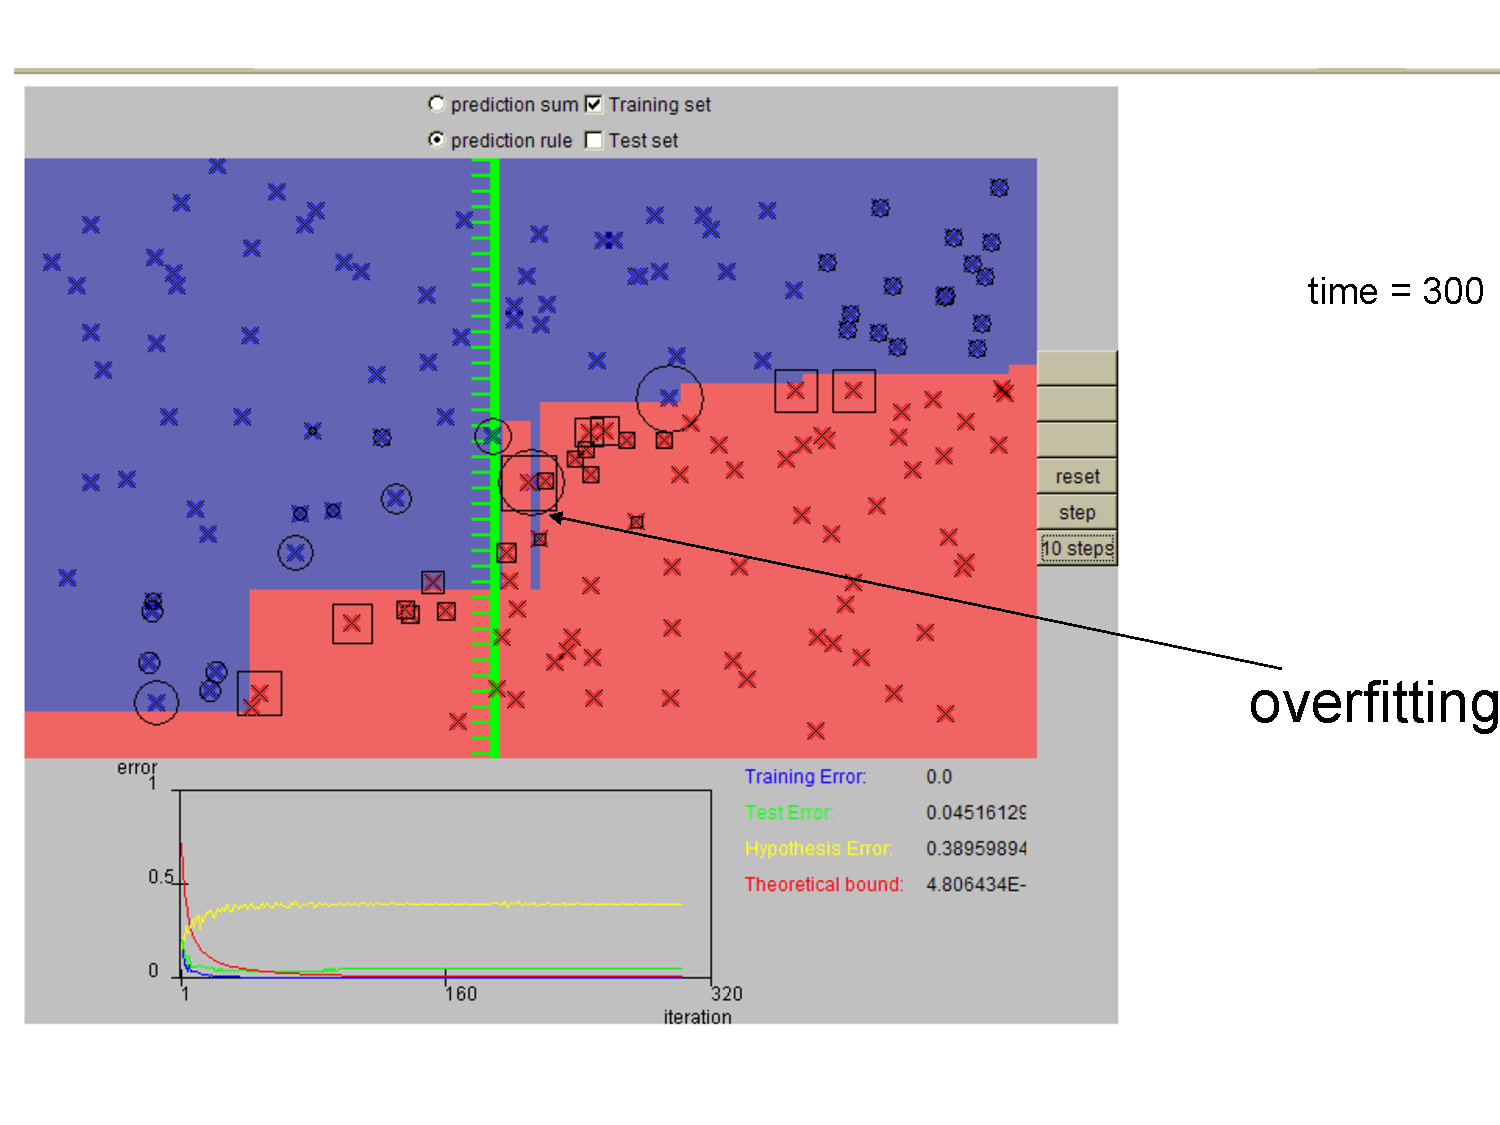
\includegraphics[width=2.5in]{figures/bagging_example.pdf}  \hfill \\
After making 300 classifiers, we can get a step-like decision boundary.  
Stopping at 100 would have been better; it is not over-fit (not shown).  \hfill \\

The blue, green, yellow, and red lines:   % I e-mailed the forum to figure this out. 
\begin{itemize}
	\item blue = training error = same as usual.  Randomly choose a subset to hold-out for testing
	\item green = test error = same as usual.  Randomly choose a subset to hold-out for testing
	\item yellow = hypothesis error = the error of the new weak learner generated on that step 
			(i.e. a decision stump) \hfill \\
		"Last classifier we added was 38\% wrong. " 
		for time = 100 when Hypothesis error said 0.38
	\item red = theoretical bound = the bound on the training error, derived in the later slides
\end{itemize}
% TA: Training/test sets are selected as always: randomly choosing a subset to hold-out for testing. Hypothesis error tells you the error of the new weak learner generated on that step (i.e. a decision stump). Theoretical bound is the bound on the training error, derived in the later slides.

\subsubsection{Learning from weighted data}  
Consider a weighted data set: \hfill \\
\begin{itemize}
	\item $D(i)$ is the weight of the $i^{th}$ training example/point (not classifier!). 
		It gets bigger each time point $i$ is predicted incorrectly.  
		It doesn't get smaller, but you normalize (see below). 
		\hfill \\
		Point = $(\bm{x}^i, \bm{y}^i)$
	\item interpretations:
		\begin{itemize}
			\item the $i^{th}$ training example counts as if it occurred $D(i)$ times
			\item these extra counts mean that if we were to "resample" data, 
				we would get more samples of "heavier" data points. 
		\end{itemize}
	\item Now we always do weighted calculations:
		\begin{itemize}
			\item e.g. MLE for Naive Bayes
			\item redefine Count(Y=y) to be a weighted count: \hfill \\
				$\displaystyle Count(Y=y) = \sum_{j=1}^n D(j) \delta (Y^j = y)$
			\item ?? Is this counting the number of points we have right?? No.. what is it counting? 
			\item if point $j$ has been wrong many times before, 
					it becomes more important, as reflected by $D(j)$ being large. 
			\item setting $D(j) = 1$ (or any constant value!) for all $j$ recreates the unweighted case. 
		\end{itemize}
\end{itemize}


Note, we can use decision stumps for boosting.  Can also use logistic regression, but it isn't as easy to show as our clas stump example.  \hfill \\
\hfill \\

That's just about weighing the samples.  How do we weight the classifiers? 
We want to weight across \underline{all} data points. 
Use $\alpha$ to allow classifiers to have different votes. 

\subsubsection{Algorithm: Binary case}
\underline{Given}: points $(x^1, y^1), \dots, x^m, y^m$.  \hfill \\
For this case, $x^i \in \mathbb{R}$, and binary labels: $y^i \in \{-1, +1\}$ \hfill \\
\underline{Initialize}: $D_1(i) = 1/m$ for $i=1, \dot, m$.  \hfill \\
For $t = 1, \dots, T:$
\begin{itemize}
	\item Train base classifier $h_t(x)$ using $D_t$
	\item Chose the weight of importance for this classifier, $\alpha_t$. \hfill \\
		Note that this comes after training the classifier.  \hfill \\
		There are many possibilities for choosing $\alpha$, which are discussed later.  \hfill \\
	\item Update, for $i= 1 \dots m$:  \hfill \\
		$D_{t+1}(i) \propto D_t(i) exp(-\alpha_t y^i h_t(x^i))$ \hfill \\
				with normalization constant $\displaystyle \sum_{i=1}^M D_t(i) \exp(-\alpha_t y^i h_t(x^i))$ 
		\begin{itemize}
			\item The $D$ is getting reweighted for the next round.  \hfill \\
			What's happening inside: \hfill \\
			If $y^i h_t(x^i) > 0$, $h_i$ was correct.  \hfill \\
			But if $y^i h_t(x^i) < 0$, $h_i$ was wrong.  \hfill \\
			You multiply by $\alpha_t$, which can flip the sign inside the $\exp()$. \hfill \\
			If $h_i$ is correct and $\alpha > 0$, then $D_{t+1}(i) < D_t(i)$.  \hfill \\
			But if $h_i$ is wrong and $\alpha > 0$, then $D_{t+1}(i) > D_t(i)$.  \hfill \\
		\end{itemize}
	\item Output a final classifier: $\displaystyle h = sign \left( \sum_{i=1}^T \alpha_t h_t(x) \right)$ \hfill \\
		This is a linear sum of "base" (weak) classifier outputs. \hfill \\
		Note that $D$ is no longer in the picture. 		
\end{itemize}
If you had two classifiers, your result would be $\alpha_1 h_1 + \alpha_2 h_2$

\textbf{How to chose $\alpha$}: \hfill \\
First calculate $\displaystyle  \epsilon_t = \sum_{i=1}^m D_t(i) \delta(h_t(x^i \neq y^i)))$ \hfill \\
This is the error of $h_t$, weighted by $D_t$ \hfill \\
Then use $\displaystyle  \alpha_t = \frac{1}{2} \ln \left( \frac{1 - \epsilon_t}{\epsilon_t} \right)$  (derived below) \hfill \\
This transforms alpha according to:  \hfill \\
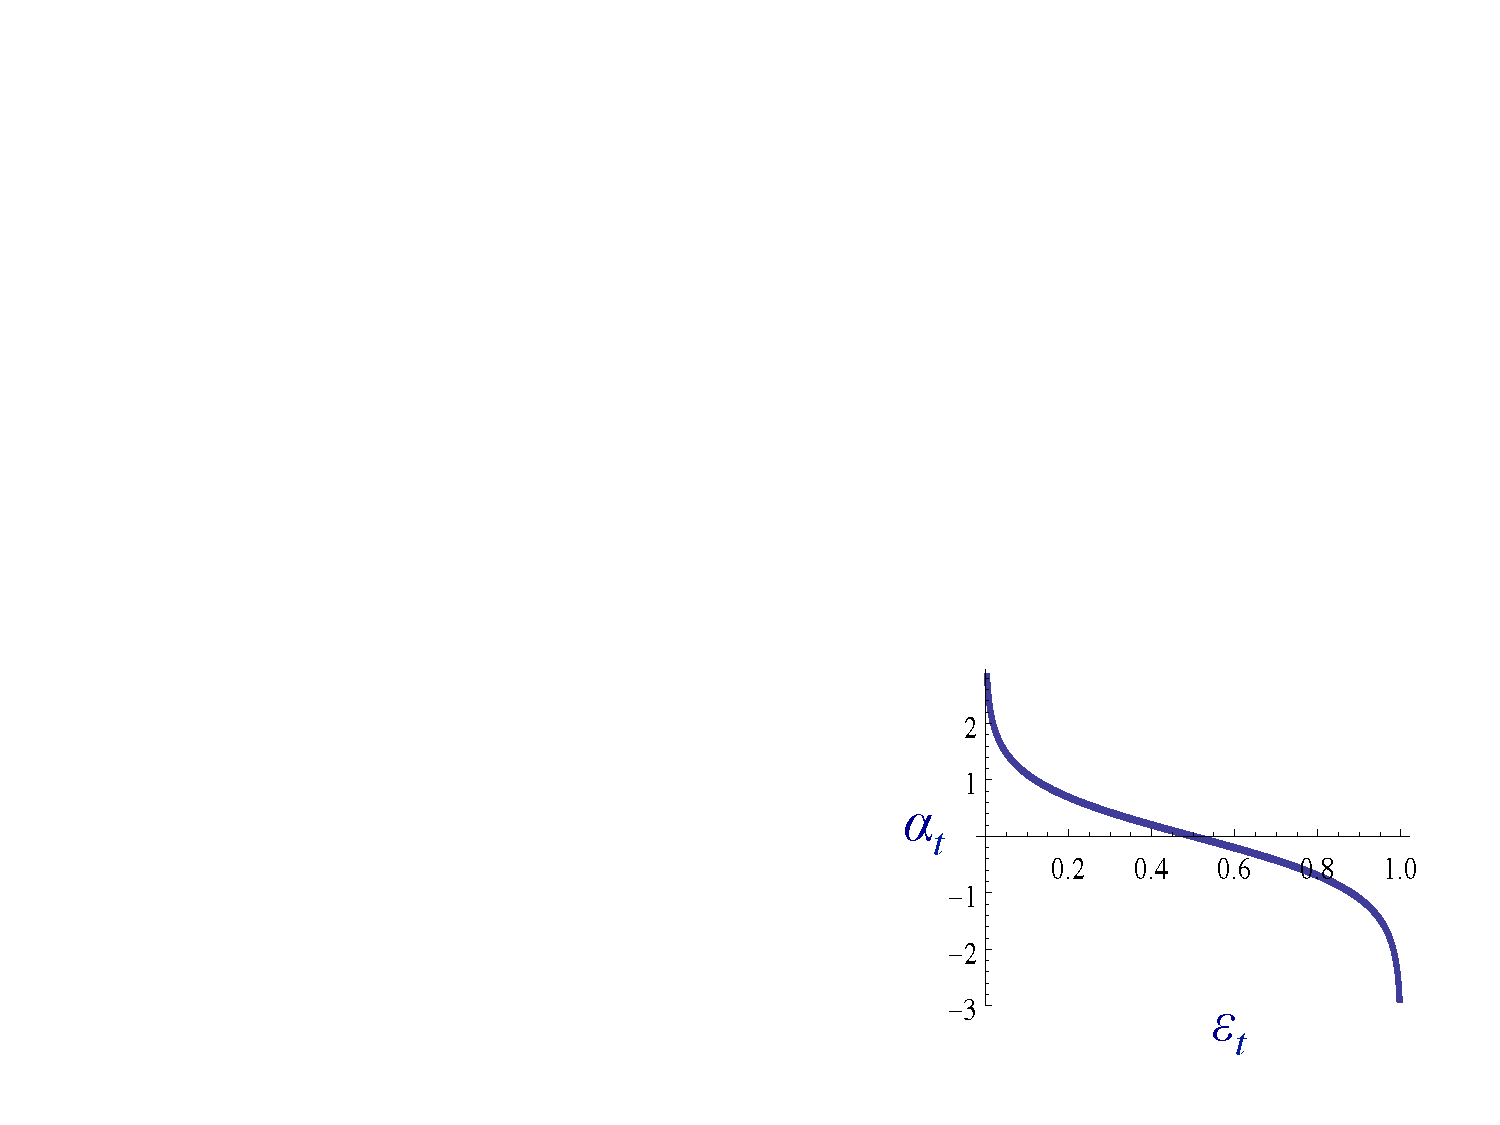
\includegraphics[width=1.2in]{figures/alpha_from_epsilon.pdf}
\begin{itemize}
	\item no errors:  $\epsilon_t = 0 \rightarrow \alpha_t = \infty$
	\item all errors:  $\epsilon_t = 1 \rightarrow \alpha_t = -\infty$
	\item random:  $\epsilon_t = 0.5 \rightarrow \alpha_t = 0$
\end{itemize}
Truncate at 2 or 3.  Don't want to allow weight = infinity. \hfill \\  % week 9 audio
Think of this like NB with weighting. \hfill \\  % week 8 audio.
\underline{Why would we want/have negative weights on classifiers?} \hfill \\
A classifier that does worse than chance is backwards. 
If it is worse than chance, flip the sign then use it. 
A classifier that is wrong 90\% of the time is a good classifier.   
A truly random classifier does not provide information.  Thow those away.

\hfill \\
If you get something right a bunch of times, the weight should converge to zero.  % week 8 audio
\hfill \\

We want to run this loop until it converges.  
But if we run it too long, it will overfit. 

\subsubsection{How to chose $\alpha_t$ for hypothesis $h_t$?}
It would be cool to find the $\alpha_t$ that works best for that classifier, take derivative with respect to $\alpha_t$, and find an $\alpha$ that minimizes error. \hfill \\
We can't optimize the training set error, but we can minimize a bound on it. \hfill \\
$\displaystyle  \sum_{i=1}^m \delta(H(x^i) \neq y^i) \leq \sum_{i=1}^m D_t(i) \exp(-y^i f(x^i))$ \hfill \\
where $\displaystyle f(x) = \sum_t \alpha_t h_t(x)$; $H(x) = sign(f(x))$ \hfill \\
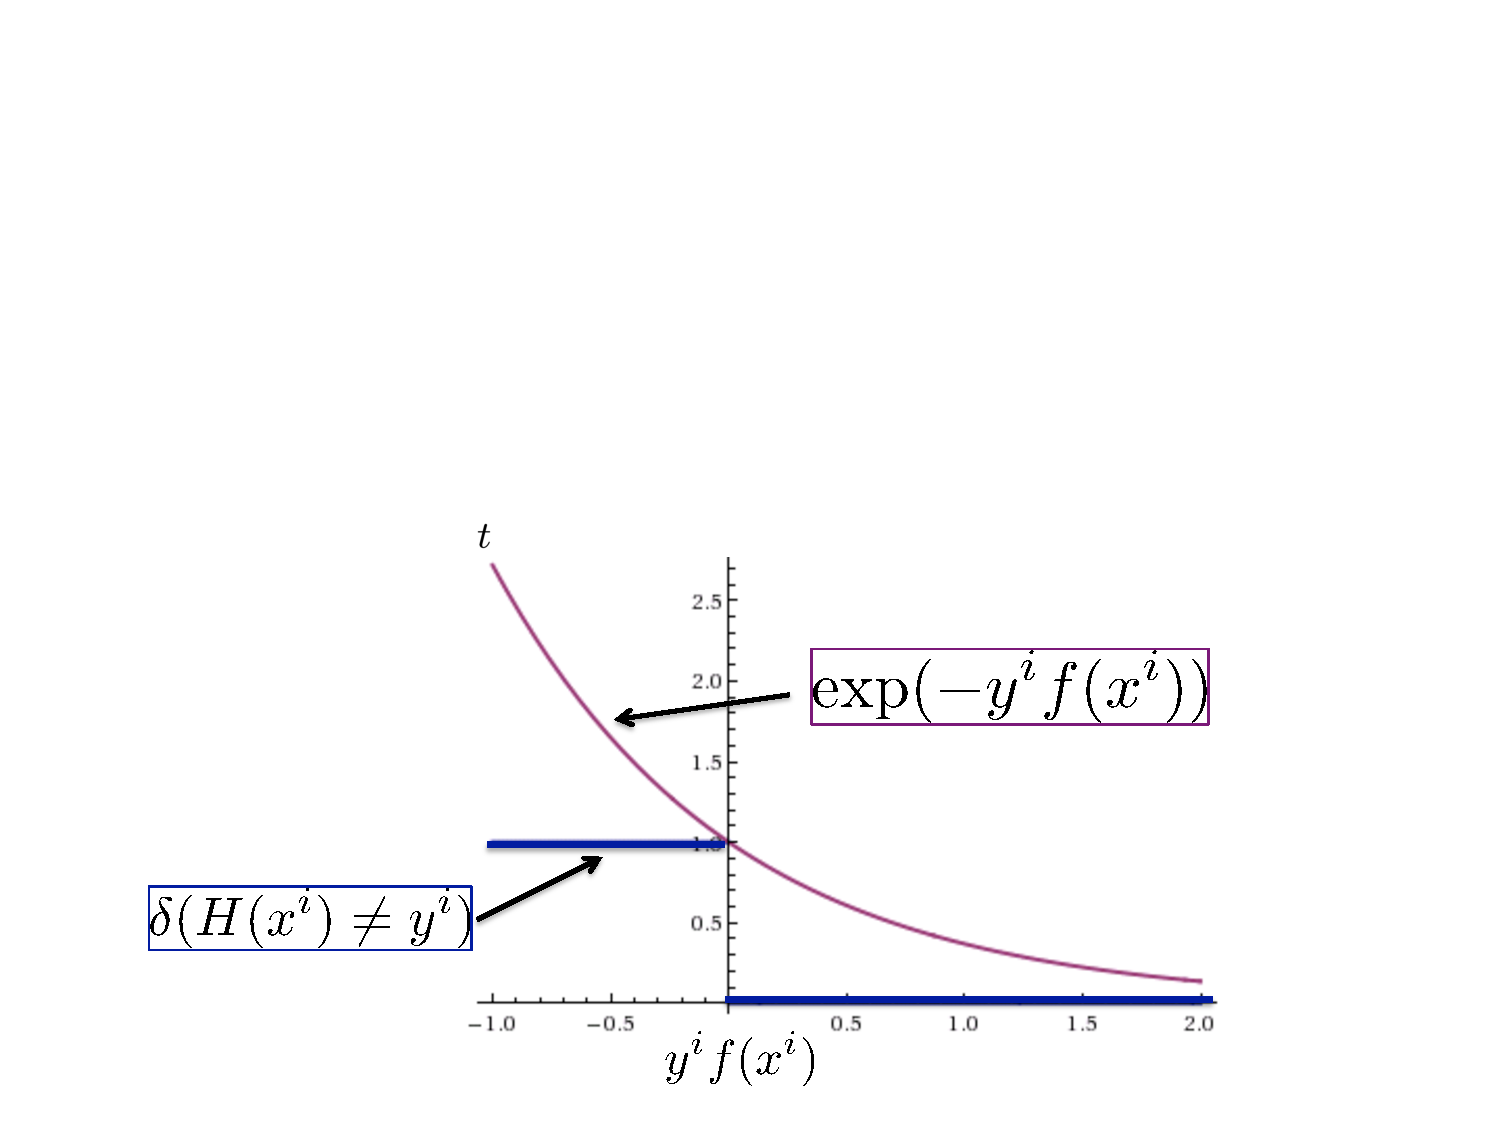
\includegraphics[width=2.5in]{figures/chosing_alpha_step_func.pdf}
 
We know the training set error (\# of instances wrong) it is bounded by the sum on the right.
Why?  The left side of the equality is the left piece of the step function.
The exponential function of label*prediction has the expo curve.
Note that \textbf{the exponential curve is always above the step function}.
So we can use expo as the upper bound. 
This is kind of like logistic regression: same form.

% --------
\subsubsection{You can choose $\alpha_t$ to minimize the error bound.}
Note that each classifier is independent of alpha.  
Each classifier is already a classifier by itself. 
We want to train the weighted combinations of classifiers.  
Note we are not directly using the error.  
We are using a function that maps the error to a \# we can use. 
That's the role of the alpha vs epsilon curve.  
We liked its properties. 
There are two parameters in the $\exp()$:  $h$ and $\alpha.$
You can optimize for h and alpha together.
We have a way to make the classifier sand learn the weights at the same time.
We might still learn the classifiers first. 
For those of you who care about joint optimization, you can flip between optimizing the two. 

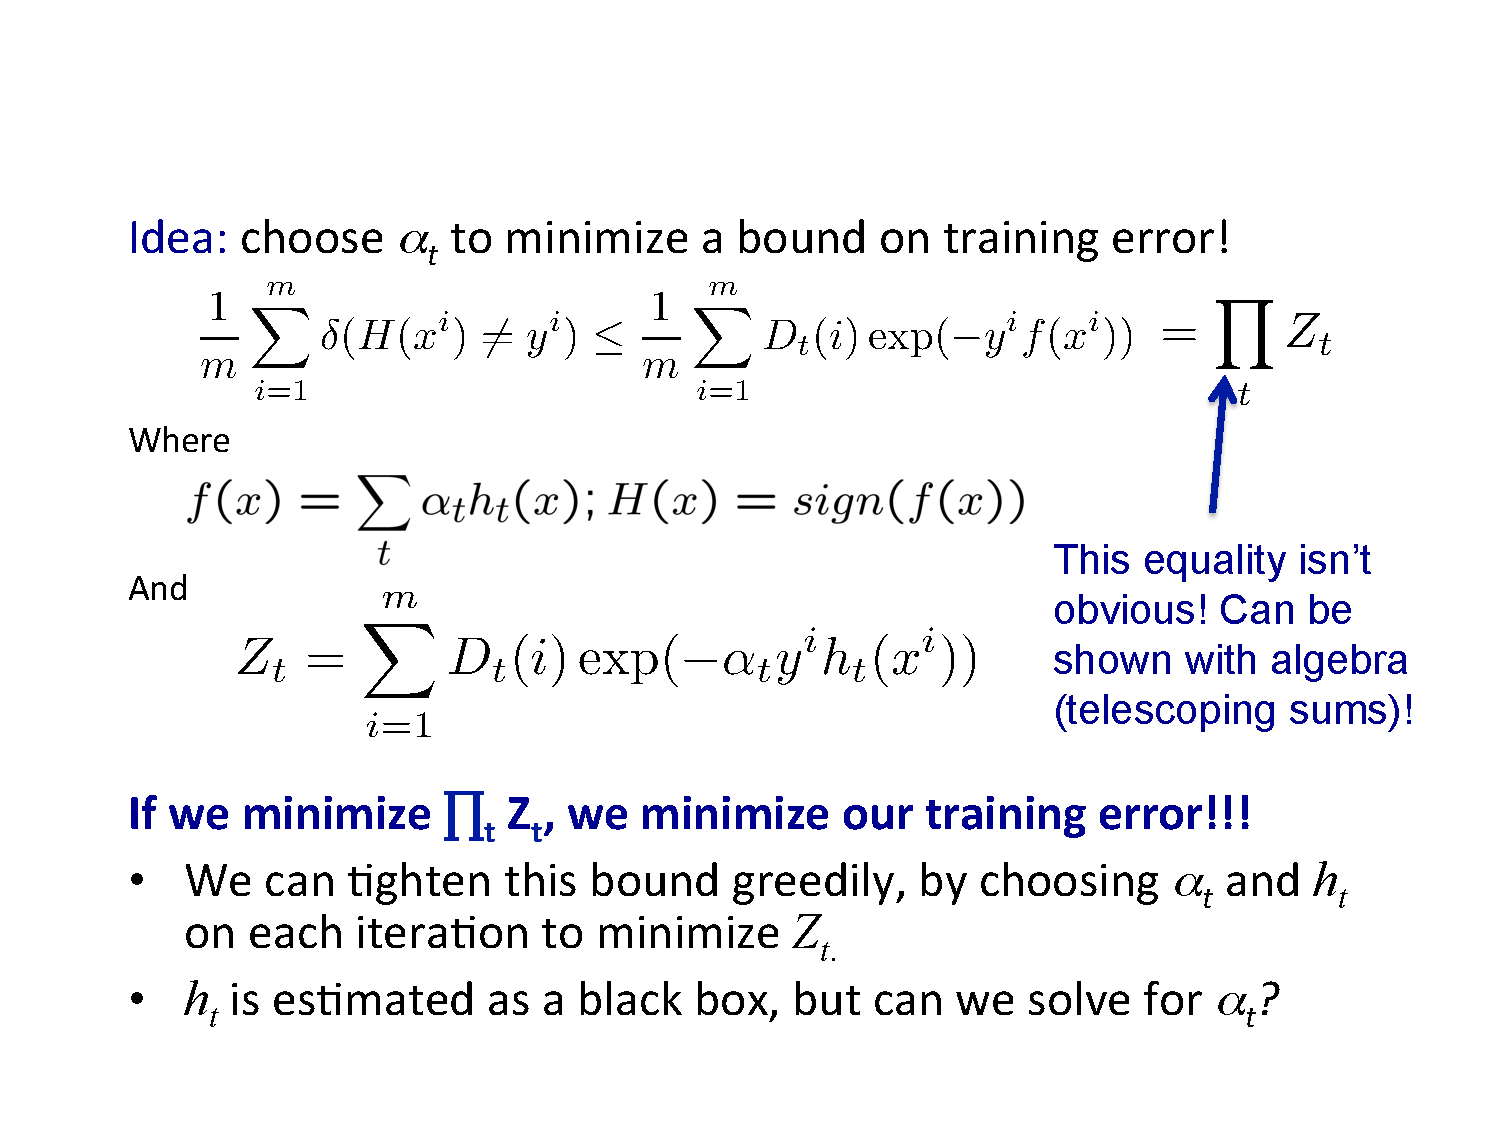
\includegraphics[width=2.7in]{figures/chosing_alpha--telescoping_sums.pdf}

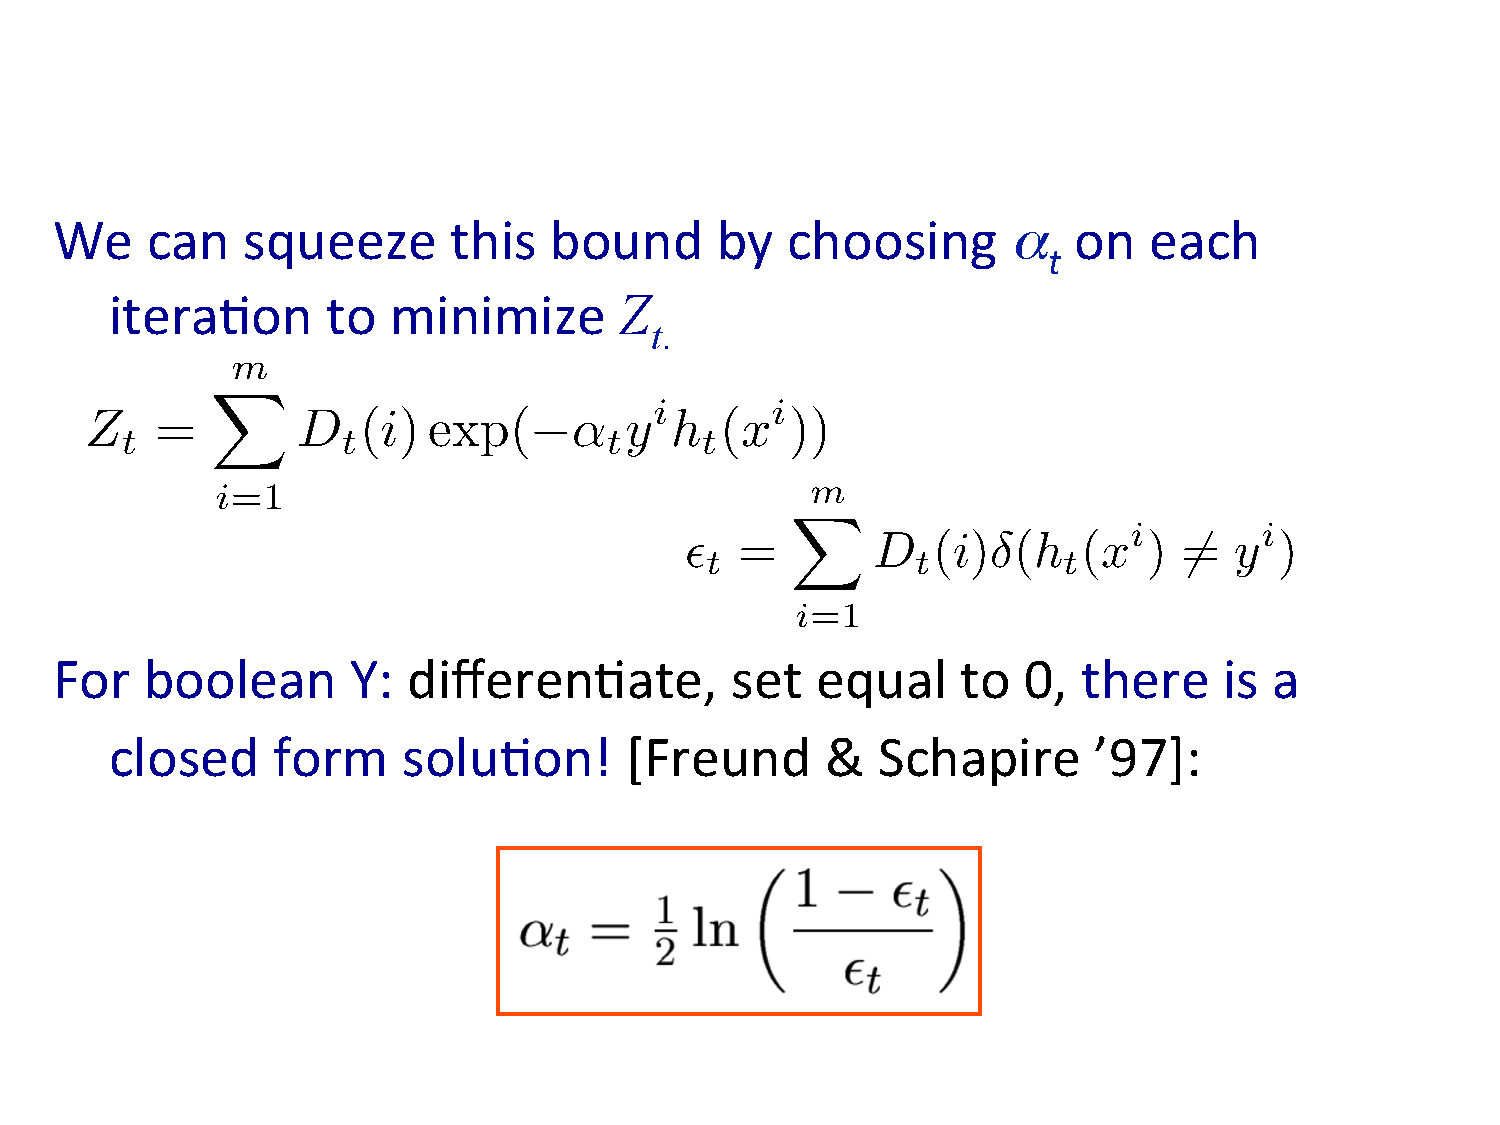
\includegraphics[width=2.7in]{figures/chosing_alpha--telescoping_sums2.pdf}

Note that our $D$ values are not going up by more than 1 each time, like the intro to the concept showed.
There is an exponential term that generally shrinks the sum of the $D$ values to 1 (at least in the class example).  \hfill \\
\hfill \\

After the third iteration for our class example:
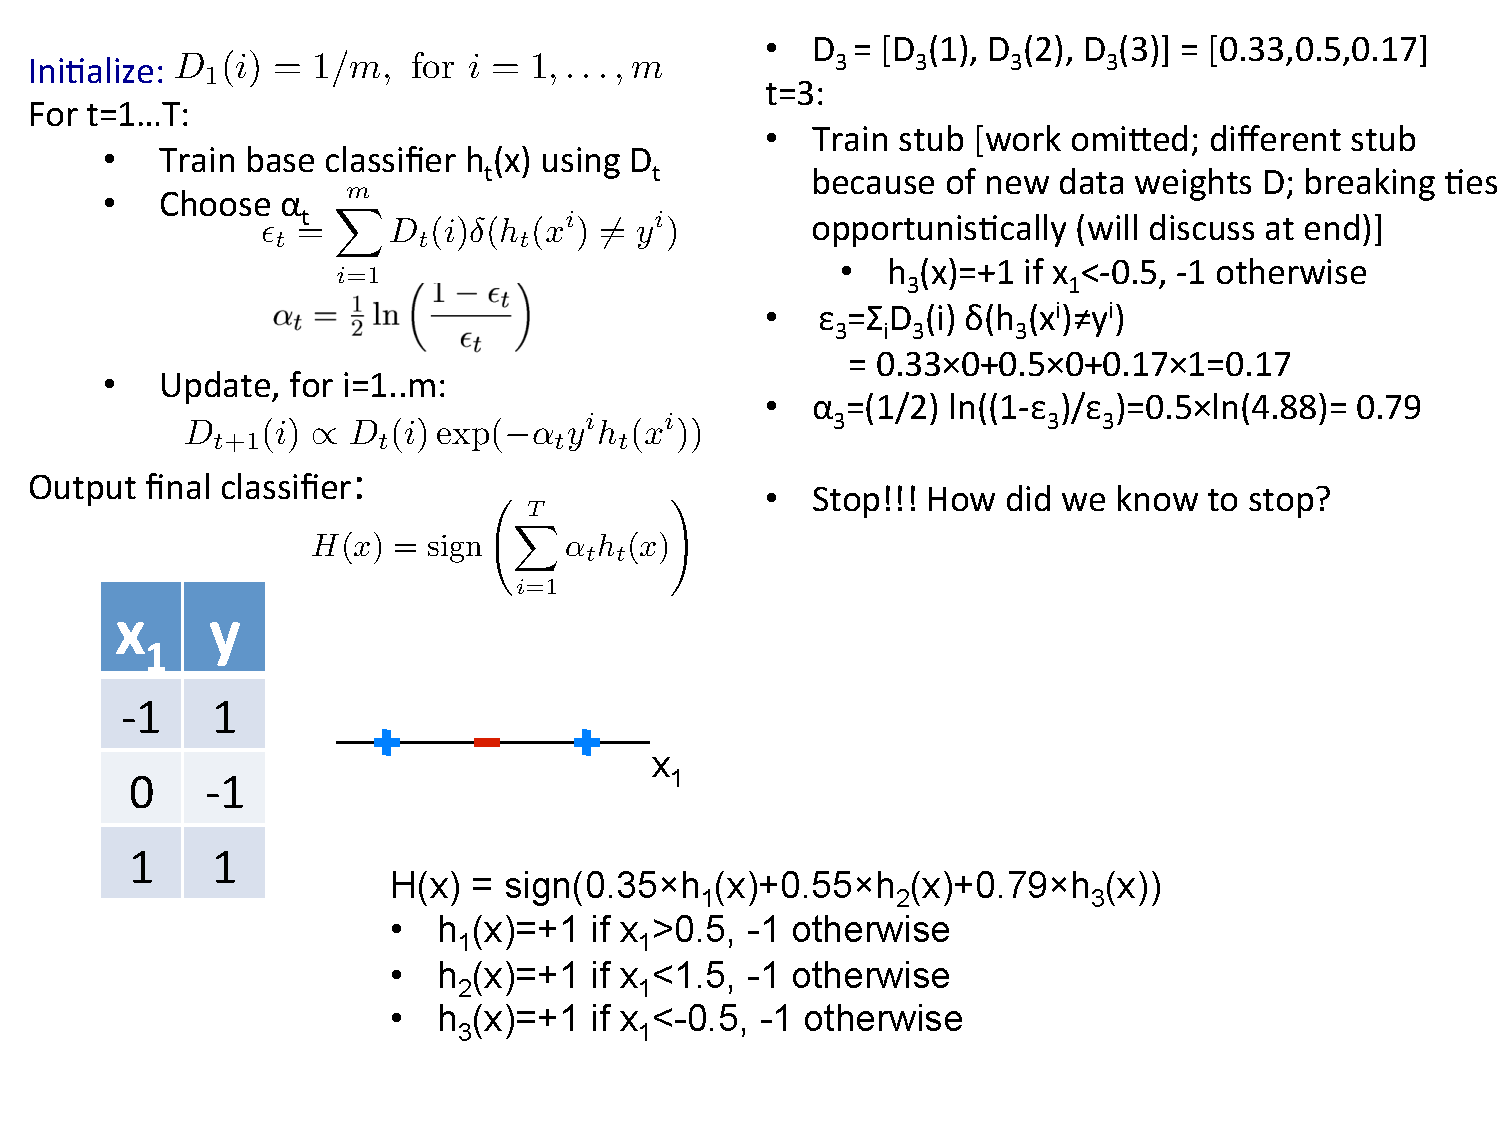
\includegraphics[width=3.4in]{figures/boosting_example_3rd_iteration.pdf} \hfill \\
The $\epsilon$ values are dependent on the previous iteration's $D$ values, 
	but the current iterations $h$ classifier. \hfill \\
Once you find your new $\epsilon$ from your old $D$s and new $h$, 
	you can find $\alpha$ and thus your new $D$s for the next round.   \hfill \\
%?? Does your previous classifier know anything about your other classifiers ??    \hfill \\
%?? Should we think of the fact that it was trained using $D$s from previous classifiers as knowledge about other classifiers ??   \hfill \\
?? Is it typical to have your alpha weights grow ??  Can I explain what is driving this ?? 
\hfill \\
\hfill \\

\textbf{The D after normalization is a probability.}

\subsubsection{Assembling weak classifiers}
If each classifier is (at least slightly) better than random: $\epsilon_t < 0.5$: \hfill \\
Another bound on error:
$$ \frac{1}{m} \sum_{i=1}^m \delta (H(x^i) \neq y^i) \leq \prod_t Z_t \leq \exp \left( -2 \sum_{t=1}^T (\frac{1}{2} - \epsilon_t)^2 \right)$$
This implies training error will reach zero exponentially fast. \hfill \\
The error is bounded by an exponential of how far you are from random. \hfill \\

Note that it isn't too hard to achieve better than random training error, especially for binary classification.   \hfill \\
Boosting is powerful!  \hfill \\

Note that test error can continue to decrease after training error goes to zero.  

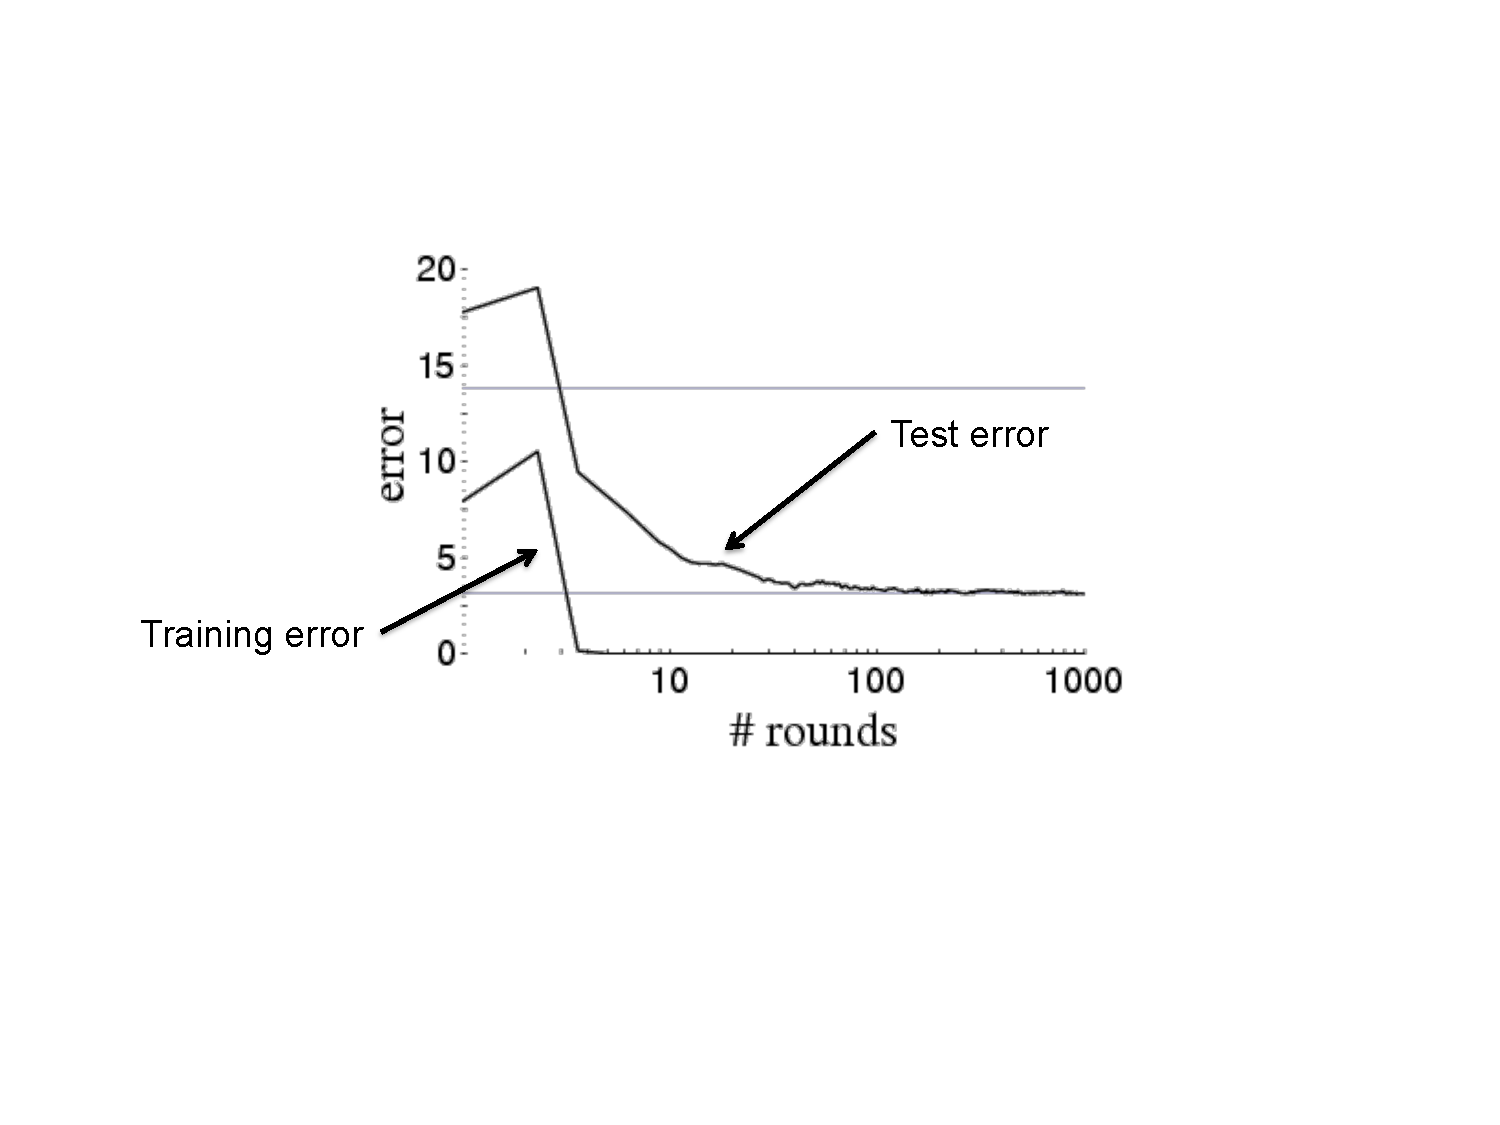
\includegraphics[width=2.2in]{figures/boosting_train_test_error.pdf}

Also in this figure, the lack of up-tick at the right shows that boosting does not overfit. 

\subsubsection{Using your classifier}
Say you have a trained/converged classifier.
That means you have $h$s and $\alpha$s : weak classifiers and their corresponding weights. 
Plug in new $x$ into $H(x)$ %, which puts into $H(x)$.

\textbf{How do we know when to stop? } \hfill \\
If the training error keeps getting better we keep going.
This could lead to over-fitting, but it turns out boosting is robust to overfitting.   \hfill \\
(We didn't actually conclude when to stop in class.) 

There was a theory (Freund \& Schapire, 1996) that suggested 
$$ error_{true}(H) \leq error_{train}(H) + \tilde{\mathcal{O}} \left( \sqrt{\frac{Td}{m}} \right) $$
Suggests you don't want to use complicated classifiers in your boosting.  d would get high, we could end up over-fitting. % week 9 audio

$T$: number of boosting rounds.  Higher $T$ $\rightarrow$ looser bound.  \hfill \\
$d$: VC dimension of weak learner.  Measures complexity of classifier.  \hfill \\
$m$: number of training examples.  More data $\rightarrow$ tighter bound.  \hfill \\
\hfill \\

It turns out boosting is robust to overfitting.  The test set error decreases even after the training error reaches zero.  So this theory doesn't hold. 

\subsubsection{Boosting and Logistic Regression}
Both smooth approximations of 0/1 step loss.

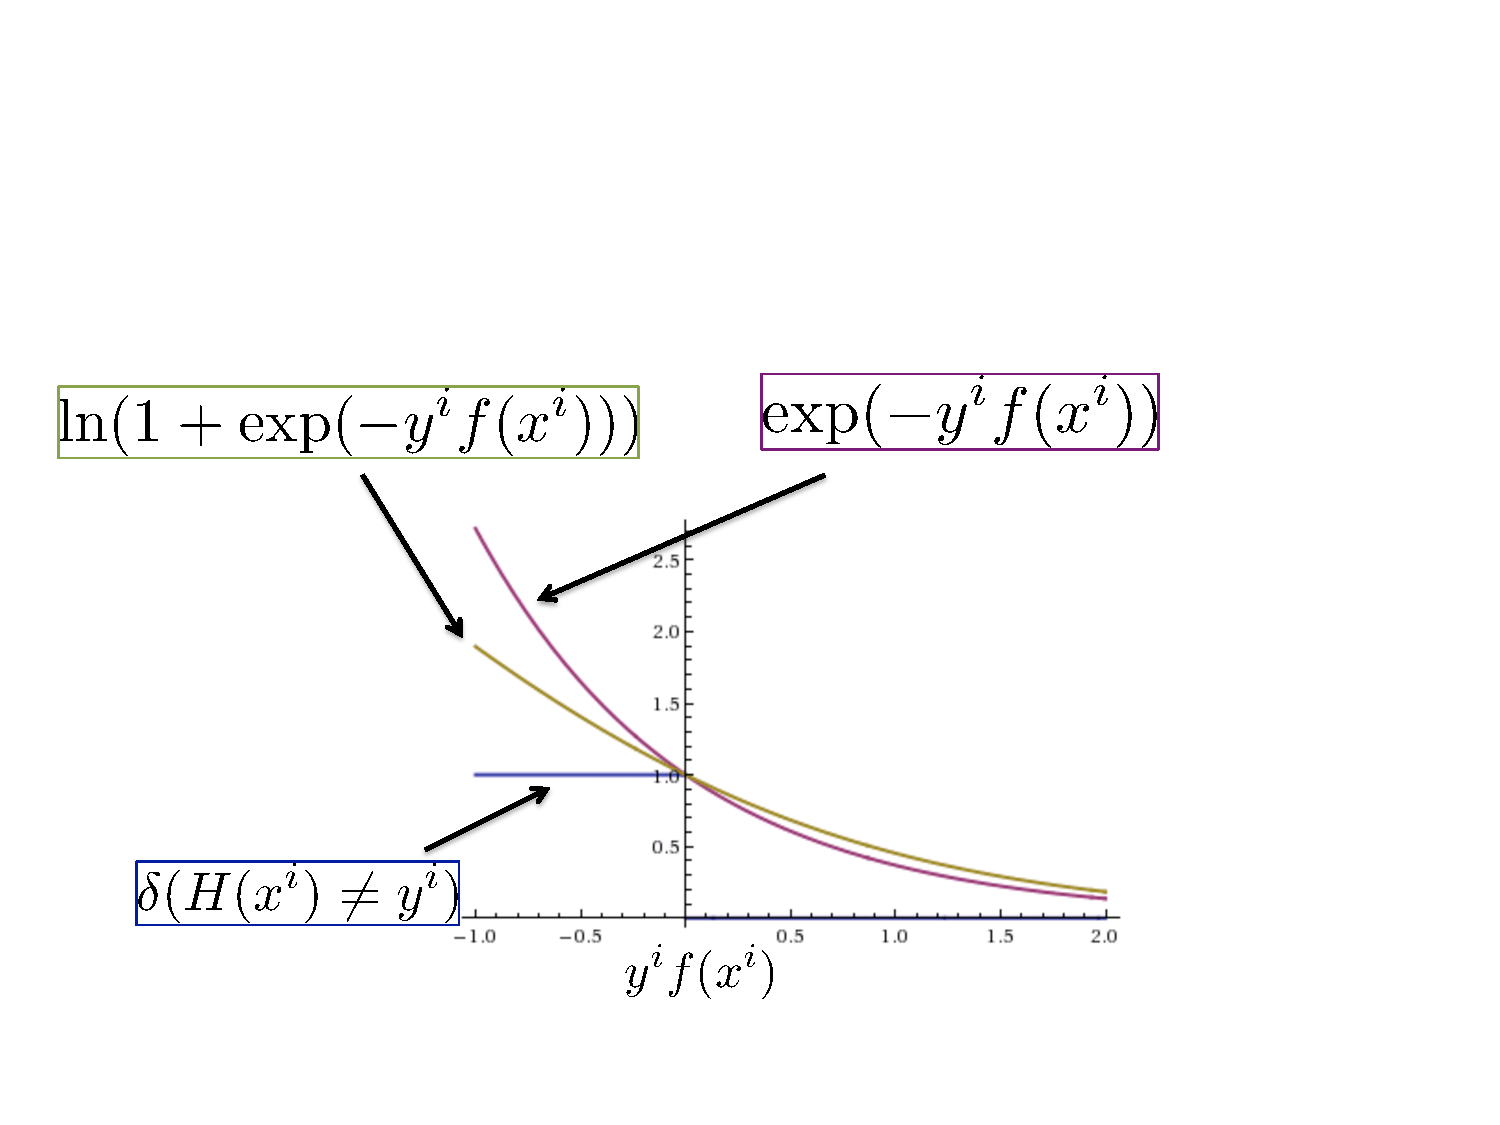
\includegraphics[width=2.2in]{figures/losses--boosting_and_logistic_regression.pdf}

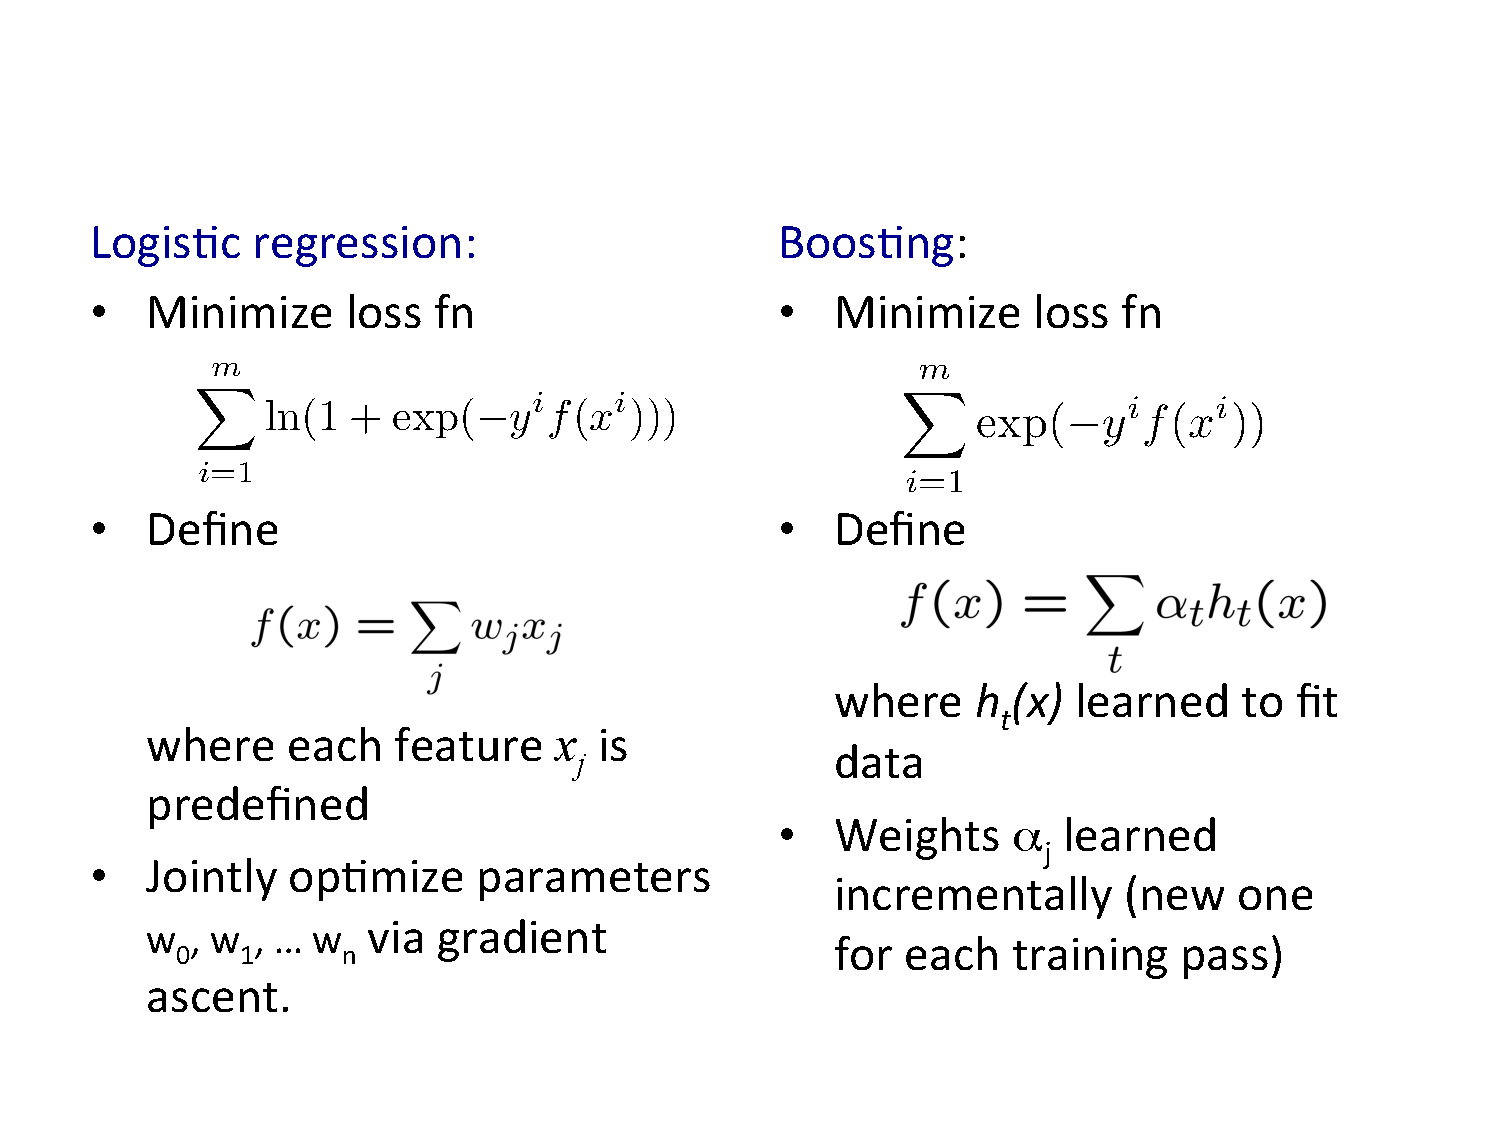
\includegraphics[width=2.7in]{figures/logistic_regression_and_boosting_summary.pdf}

As noted above:
Similar to logistic regression:
\begin{itemize}
	\item both linear models.  Boosting "learns" features.  
	\item similar loss functions
	\item single optimization (Logistic Regression) versus incrementally improving
\end{itemize} 



\section{Clustering}
\smallskip \hrule height 2pt \smallskip

\begin{itemize}
	\item Unsupervised learning: detect patterns in unlabeled data. 
		Sometimes labels are too expensive, unclear, etc. to get them.
		Examples:
		\begin{itemize}
			\item group e-mails or search results
			\item find categories of customers
			\item detect anomalous program execuations
		\end{itemize}
	\item Useful when you don't know what you are looking for. 
	\item Requires a definition of "similar".  One option: small (squared) euclidean distance. 
	\item You can label then use the clusters, or use the clusters for the next level of analysis.
\end{itemize}

\subsection{K-Means}
\begin{itemize}
	\item An iterative clustering algorithm.  \hfill \\
	\item No step size.  Discrete optimization. 
	\item Hard assignments.  Each point gets classified by one and only one cluster. 
	\item will converge, but may converge on local (not global) optimum.
		\begin{itemize}
			\item Every time you start the algorithm, you could end up n a different place.
			\item Can run it a bunch of times. % week 9 audio
			\item you are running a non-convex optimization: your final output is dependent on your initialization.
		\end{itemize}
	\item you have to chose a number of clusters. 
	\item Objective: minimize the distances between each point and closest center. 
	\item You want your output to have a large distance between clusters and a small distance between points in a cluster.  (intra vs inter cluster distance).
	You want it to latch onto clumps of the data that are far apart from each other. % week 9 audio
		\begin{itemize}
			\item intra: \hfill \\
				E.g. measure $|x_i - c_i|_2^2$ for each cluster. 
			\item inter:  \hfill \\
				Dist between closest two points in different clusters. \hfill \\
				Distance between means.  \hfill \\
				Standard deviation of cluster distances. \hfill \\
		\end{itemize}
\end{itemize}	
	
Pick K random points as cluster means: $c^1, \dots, c^k$.  \hfill \\
Alternate:
\begin{itemize}
	\item Assign each example $x^i$ to the mean $c^i$ that is closest to it
	\item Set each mean $c^i$ to the average of its assigned points. 
\end{itemize}
Stop when no points' assignments change. \hfill \\

Minimizing a loss that is a function of the points, assignments, and means:
$$ L( \{ x*i \},  \{ a*j \},   \{ c*k \}) = \sum_i dist(x^i, c^{a^i})$$
Coordinate gradient descent on L.  \hfill \\

More formally: 
\begin{itemize}
	\item Data: $\{ x^j | j = 1 \dots n \}$
	\item For $ t = 1 \dots T$:  (or stop if assignments don't change): \hfill \\
		Fix means ($c$) while you change the assignments ($a$): \hfill \\
		\begin{itemize}
			\item for $ j = 1 \dots n$: (recompute cluster assignments):
				$$ a^j = \argmin_i dist(x^j, c^i)  $$ 
		\end{itemize}
	\item fix assignments ($a$) while you change the means ($c$): \hfill \\
		for $j = 1 \dots k$: (recompute cluster centers)
		$$ c^j = \frac{1}{|\{ i | a^i = j \}|}  \sum_{\{ i | a^i = j \}} x^i$$
\end{itemize}
Note:  the point y with minimum squared Euclidean distance to a set of points {x} is their mean

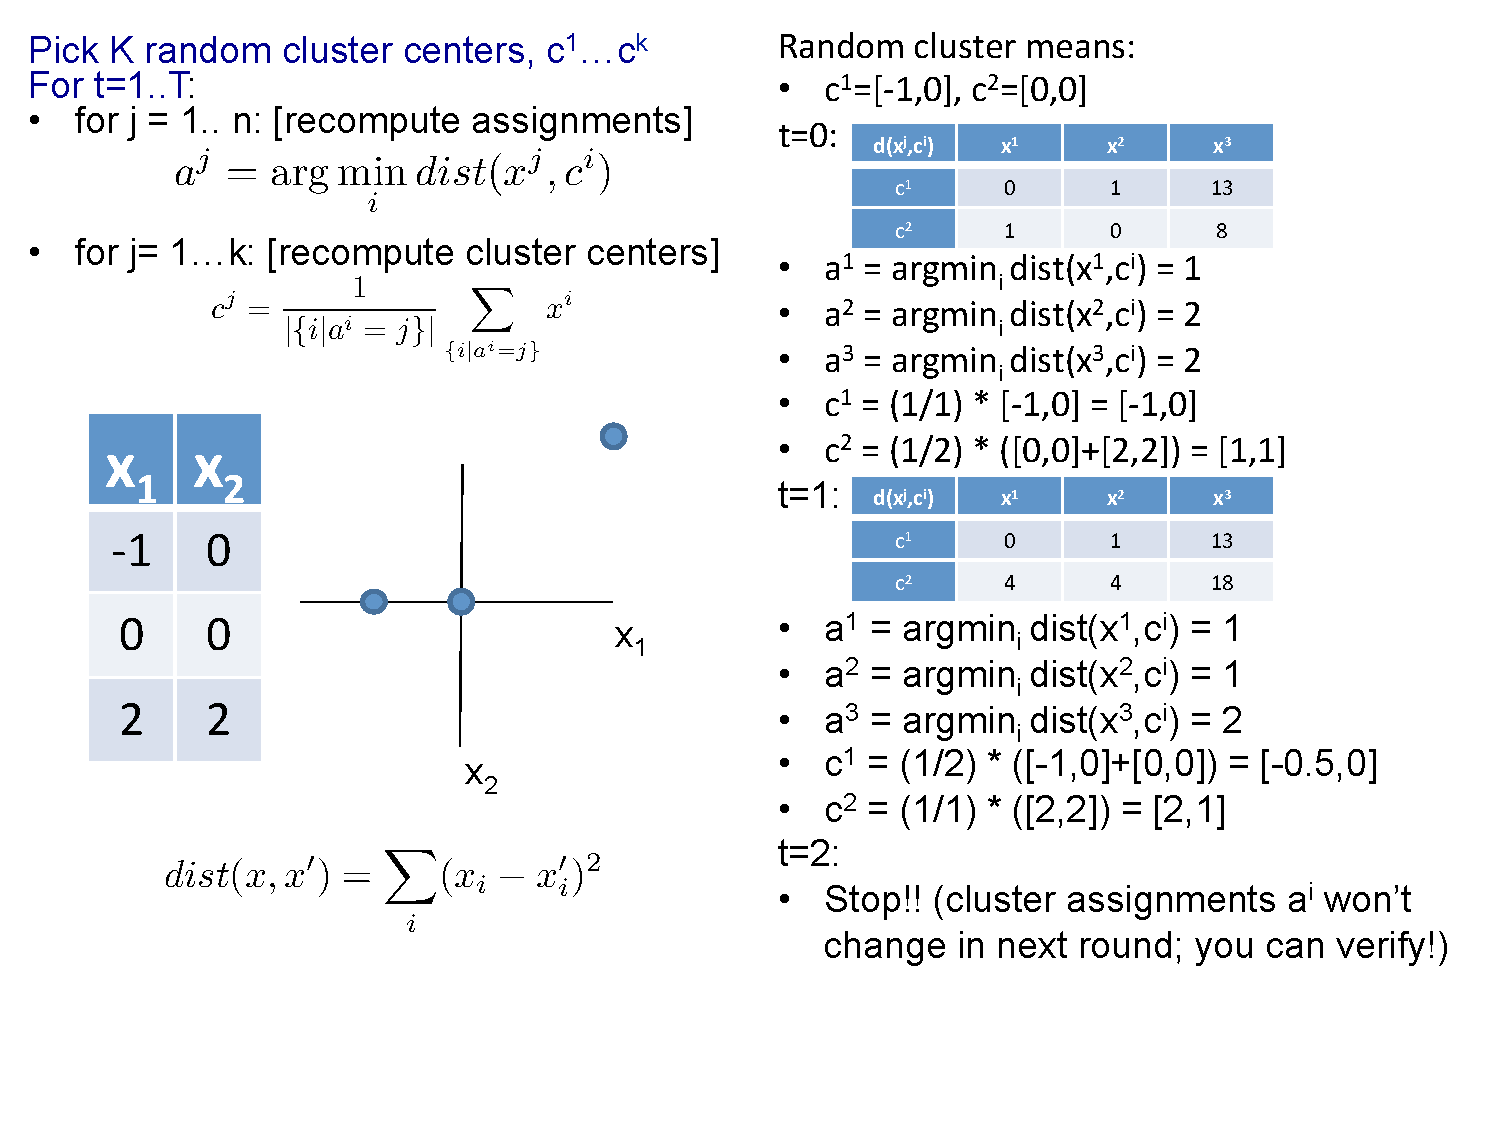
\includegraphics[width=3.6in]{figures/kmeans_algorithm_example.pdf}

\subsubsection{K-Means gets stuck in local optima.}

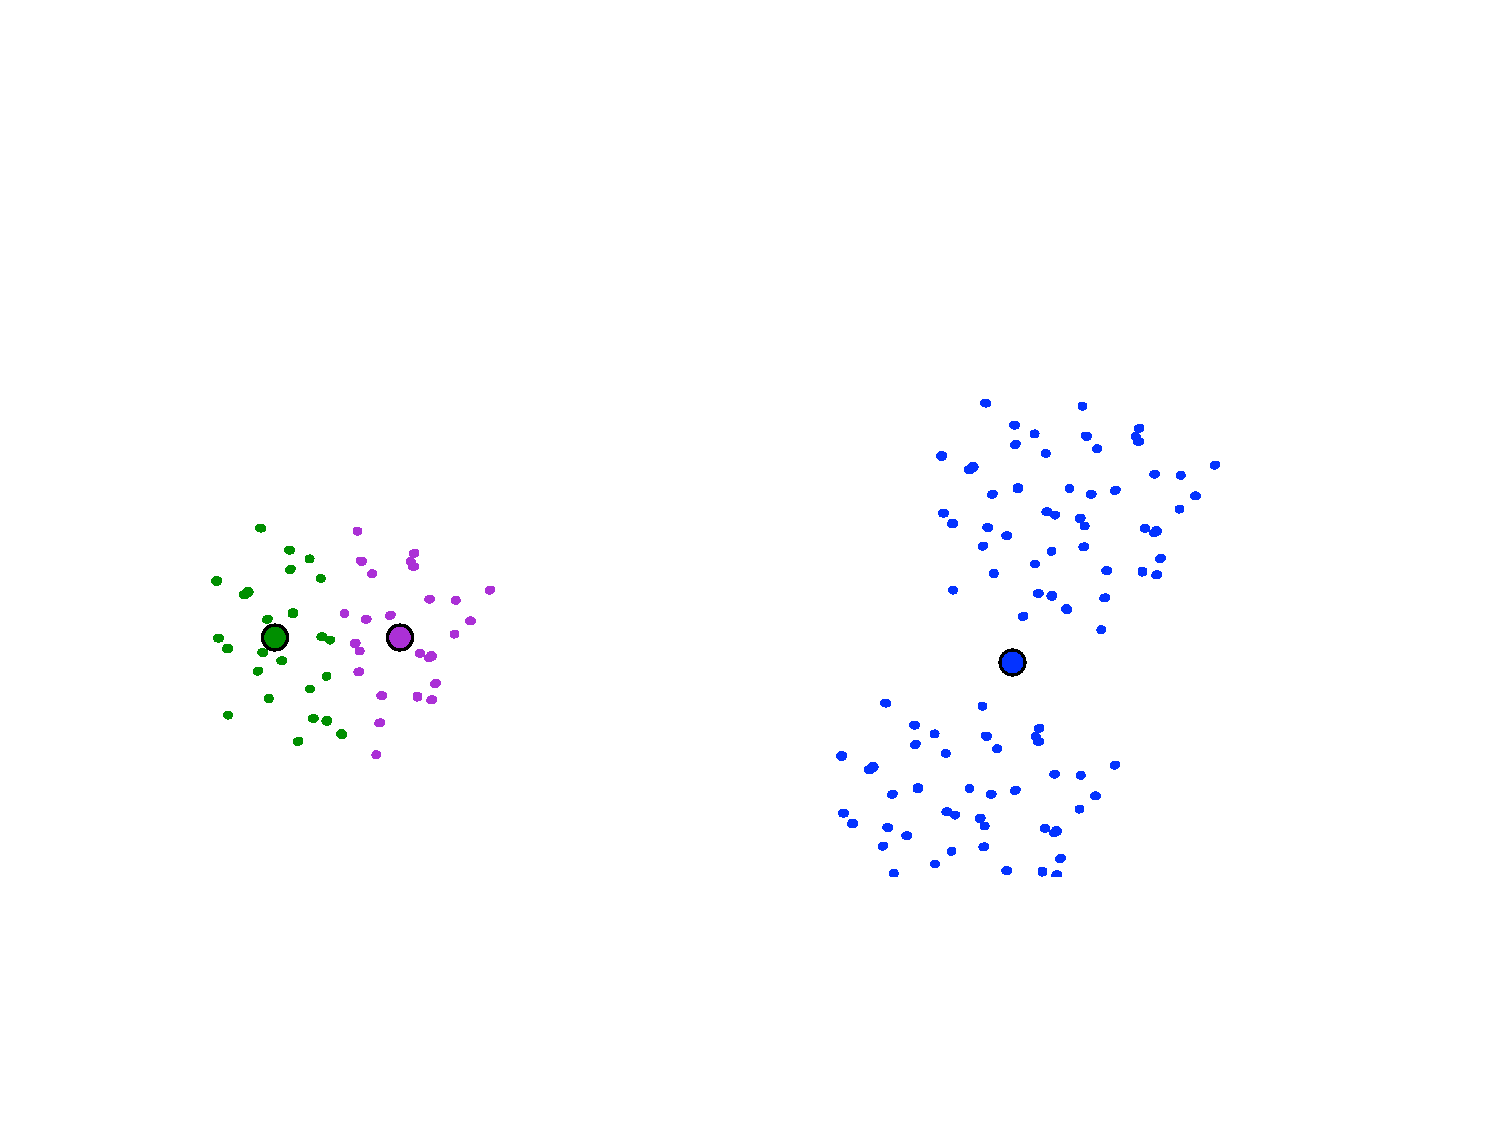
\includegraphics[width=1.8in]{figures/k-means_gets_stuck.pdf}

\subsection{Agglomerative Clustering}
Will not converge to a global optimum. \hfill \\  % TA 3/15/2016
Will not always find the true patterns in the data.  \hfill \\  % TA 3/15/2016
It has to deal with the issue of local optima just like k-means (which can prevent you from finding the "true" patterns)


First merge very similar instances. \hfill \\
Then incrementally build larger clusters out of smaller clusters. \hfill \
Limiting the number of pairs of pairs, we can control the number of clusters.
\begin{itemize} 
	\item Distance = 0 means each point is its own cluster
        \item Distances = infinity --> all in one cluster. 
\end{itemize}

\includegraphics[width=1.0in]{figures/agg_clustering.pdf}

Algorithm:
\begin{itemize}
	\item Maintain a set of clusters.
	\item Initially each instance is its own cluster
	\item Repeat:
		\begin{itemize}
			\item pick the two closest clusters
			\item merge them into a new cluster
			\item stop when there is only one cluster left. 
		\end{itemize}
	\item produces not one clustering, but a family of clusterings represented by a dendogram.
		
		\includegraphics[width=1.0in]{figures/dendogram.pdf}
\end{itemize}

\includegraphics[width=2.7in]{figures/agglomerative_clustering_distance_options.pdf}

The intra-cluster distance: a metric of how well the clustering algorithm works
$$ S_1 = \sum_{j=1}^3 \sum_i |x_i - x_c|_2^2 + \sum_{i,j} |c_j, c_i|_2^2 $$ % wk 9 audio

You have to be extremely lucky to find a data set where the result isn't dependent on the start.

Can run it a bunch of times. % week 9 audio
For each pair of points, we have a vote:  \hfill \\
Do they belong to the same cluster? \hfill \\
Look at score from score of clustering algorithm \hfill \\
We get a full graph where edge scores are "do they belong to the same 					cluster"  (and more audio I missed?) \hfill \\
Then you need to find out which components are connected.  \hfill \\

For each pair of points, we have an edge distance.  \hfill \\
Within-cluster edges should be strong edges.    \hfill \\
This strength should be common across clustering results.  \hfill \\
Cut the graph into three pieces.    \hfill \\
The score of the cut is the summation of the edges you break.   \hfill \\
Cutting edges with small scores is good.   \hfill \\


\subsection{Probabilistic Clustering}
\begin{itemize}
	\item Can use a probabilistic model that allows cluster overlaps, clusters of different sizes, etc.
	\item You can tell a generative story for the data.  \hfill \\
		$P(X|Y) P(Y)$ is common. 
	\item The challenge: estimate model parameters without labeled data. 
\end{itemize}

\subsection{Gaussian Mixture Models}
\begin{itemize}
	\item We have clumps of data. Each clump is described with a gaussian.  % wk 10 audio
	\item Like softening k-means.  You belong to cluster 1 with a score of 0.1, cluster 2 with score of 0.3, cluster 3 with score of 0.6
	\item Think of clusters as probabilistic. 
	\item Assume m-dimensional data points.
	\item P(Y) is still multinomial, with k classes.
	\item $P(\mathbb{X} | Y=i), i=1 \dots k$ are $k$ multivariate Gaussians.
		\begin{itemize}
			\item mean $\mu_i$ is a m-dimensional vector.
			\item variance $\Sigma_i$ is an $m$ by $m$ matrix.
			\item $|x|$ is the determinant of matrix x. 
		\end{itemize}
\end{itemize}

$$ P(X=x | Y=i) = \frac{1}{\sqrt{(2 \pi)^m | \Sigma_i |}} \exp \left(  \frac{1}{2}(x - \mu_i)^T \Sigma_i^{-1} (x- \mu_i) \right) $$

\subsubsection{GMM is not Gaussian Naive Bayes}
(We did GNB before logistic regression) \hfill \\
Gaussian Naive Bayes : multinomial over clusters $Y$, Gaussian over each $X_i$ given $Y$:
$$ P(Y_i = y_k) = \theta_k $$
(Again, $\theta$ is the model parameters)
$$ P(X_i = x | Y = y_k) = \frac{1}{\sigma_{ik} \sqrt{2 \pi}} \exp \left(  \frac{-(x - \mu_{ik}^2}{2 \sigma_{ik}^2} \right) $$
? Would assume the input dimensions $X_i$ do not co-vary. \hfill \\

If the input dimensions $X_i$ do co-vary, we can use Gaussian Mixture Models. 

\subsubsection{Gaussian Mixture Model Assumption}
We want to do something like MLE but now we have multiple Gaussians. \hfill \\
You don't know which label should be used for each data point(which is red, blue, green). \hfill \\
Need to guess $k$ Gaussians without knowing the $\mu$s.  \hfill \\

You can marginalize: \hfill \\
Model probability without knowing who belongs to who: marginalize over all possible y values.   \hfill \\
You are estimating $P(X|Y)$, but you don't know $Y$.   \hfill \\
You can get rid of $Y$ and get $P(X)$ by summing over $y_i$.  \hfill \\
Get $Y$ out of the equation by summing over all possible values. \hfill \\
If it was a probability table, we would be losing a column. \hfill \\


\begin{itemize}
	\item $P(Y)$: there are $k$ components
	\item $P(X | Y)$: each component generates data from a Gaussian with mean $\mu_i$ and covariance matrix $\Sigma_i$
	\item Assume each of the features are independent of each other. \hfill \\ % week 10 audio
		Then can write down $P(X|Y)$ as prod of $P(X_i | Y)$.  \hfill \\ % week 10 audio
        		Each of them will be a Gaussian distribution. \hfill \\  % week 10 audio
	\item  Can encode the whole $P(X|Y)$ with a multi-dimensional gaussian. \hfill \\  % week 10 audio
		For 2D data, this gives a circle.  \hfill \\  % week 10 audio
		For 3D data, this gives a bump.  \hfill \\  % week 10 audio
		 When we go to 100-dim space, we also have a mu.   \hfill \\  % week 10 audio
		 	Distribution is 100-dimensional. \hfill \\  % week 10 audio
			Sigma in 100-dim space is 100 by 100 covariance matrix. \hfill \\  % week 10 audio
\end{itemize}

Each data point is sampled from a \textbf{generative process}
\begin{itemize}
	\item Pick a component at random: \hfill \\
		choose component $i$ with probability $P(y=i)$
	\item Datapoint $\sim N(\mu_i, \Sigma_i)$
\end{itemize}

\includegraphics[width=1.0in]{figures/GMM_cartoon.pdf}

\subsubsection{Supervised MLE for GMM}
(Detour/review) \hfill \\

How do we estimate parameters for Gaussian Mixtures with fully supervised data? \hfill \\
Define objective and solve optimization: \hfill \\
From above: 
$$ P(X=x | Y=i) = \frac{1}{\sqrt{(2 \pi)^m | \Sigma_i |}} \exp \left(  \frac{1}{2}(x - \mu_i)^T \Sigma_i^{-1} (x- \mu_i) \right) $$
And we know $ \displaystyle \mu_{ML} = \frac{1}{n} \sum_{i=1}^n x^i$ and $ \displaystyle \Sigma_{ML} = \frac{1}{n} \sum_{i=1}^n (x^i - \mu_{ML}) (x^i - \mu_{ML})^T$ \hfill \\

But we don't know Y, so we can't do that.  \hfill \\

Instead, we maximize the marginal likelihood.  (marginal means a variable is integrated out).
$$ \argmax_{\theta} \prod_i P(x^j; \theta) = \argmax \prod_j \sum_{i=1}^k P(y^j=i, x^j; \theta) $$

This is always a hard problem.  \hfill \\
There is usually no closed form solution.  \hfill \\
Even when $P(X, Y; \theta)$ is convex, $P(X; \theta)$ generally isn't.  \hfill \\
For all but the simplest  $P(X; \theta)$, we will also have to do gradient ascent, in a big messy space with lots of local optima.   \hfill \\

\subsubsection{Simple GMM example: learn means only}
\includegraphics[width=2.5in]{figures/gmm_for_means_only.pdf}

We solve this using EM below. 

\includegraphics[width=2.9in]{figures/learning_general_mixtures_of_Gaussians.pdf}

\subsubsection{EM for GMM: learn means of 1D data}
\includegraphics[width=2.5in]{figures/gmm--means_only-1.pdf}

\includegraphics[width=3.3in]{figures/gmm--means_only-2.pdf}

\subsubsection{EM for GMM in general}

\includegraphics[width=3.3in]{figures/EM_for_GMM.pdf}

\subsubsection{EM with hard assignments, and only learning means $\rightarrow$ K-means}

\includegraphics[width=3.3in]{figures/em_to_kmeans.pdf}




\section{Expectation Maximization}
\smallskip \hrule height 2pt \smallskip

A clever method for maximizing marginal likelihood, where you alternate between computing an expectation and a maximization. 

It is not magic: it is still optimizing a non-convex function with lots of local optima.  The computations are just easier. 

\begin{itemize}
	\item as in GMM: $$ \argmax_{\theta} \prod_i P(x^j; \theta) = \argmax \prod_j \sum_{i=1}^k P(y^j=i, x^j; \theta) $$

\end{itemize}

\section{General Vocab}
\smallskip \hrule height 2pt \smallskip
 
 \begin{itemize}
 	\item \textbf{classification} - ??? Finding a f that converts X to Y where Y are categorical.  (Not regression).  
	\item \textbf{supervised learning} - at training time we are given a set of features with discrete class labels.  % Wk 4 audio transcription.
 	\item \textbf{held-out data}: 
			the terms "held-out" and "validation" are usually synonymous  % 2/25/2015 class forum (my question)
	\item \textbf{hypothesis space}: ?  E.g. binomial distribution for coin flip.  	
 	\item \textbf{prediction error}: measure of fit (?) 
	\item \textbf{regularization}: a process of introducing additional information in order to solve an ill-posed problem or to prevent overfitting  % https://en.wikipedia.org/wiki/Regularization_(mathematics)
	\item \textbf {norm}.  A scalar (not vector!) measure of distance between two vectors.  % E confirmed 3/6/2016
					You can divide by this scalar to \underline{norm}alize, but that is just one use case.
					You can also use either norm as a regularization term. 
	\item \textbf{L1} norm.  Just add the absolute values of the components.  % E confirmed 3/6/2016
	\item \textbf{L2} norm.  Can be used to regularize, or to normalizing features. 
		\begin{itemize}
			\item Euclidean vector length.  Pythagoras style. 
			\item You can do $l_2$ normalization for a feature vector to get a unit vector: 
				Convert $x$ to $\hat{x}$ so that if you form $||\hat{x}||_2^2 = 1$
				Can also do $l_1$
		\end{itemize}
	\item \textbf{L2} distance:  Pythagoras distance between two vectors. 
	\item \textbf{convergence} - if you add more data and you don't get different parameters, the model has converged. 
	\item \textbf{kernel}: some transformation of your features that improves your classification %Erick 1/30/2015
	%\item \textbf{}
	\item \textbf{affine}: indicates that the subspace need not pass through the origin.  % Intro to statistical learning Ch 9.1
	\item \textbf{support vector}: data points that �support� the maximal margin hyperplane in the sense that if these points were 				moved slightly then the maximal margin hyper- plane would move as well.   % Intro to statistical learning Ch 9.1
	\item \textbf{marginal likelihood}: 
	\item \textbf{marginalized out} = integrated out % https://en.wikipedia.org/wiki/Marginal_likelihood

 \end{itemize}
 
 Concepts:
\textbf{likelihood vs posterior}: \hfill \\

	likelihood*prior = constant*posterior.  $P(Y|X)$ is likelihood, $P(X|Y)$ is posterior.  
\hfill \\
\hfill \\

\subsubsection{Normalizing data}
Options:
\begin{itemize}
	\item min/max
	\item sigmoid
	\item $L_1$ norm
	\item $L_2$ norm
\end{itemize}
Note $L_1$/$L_2$ normalization versus penalty/regularization!!  

\subsubsection{Size for modeling P$(Y=y | X)$}
		How many parameters are needed to model $P(y | x_1, x_2, ..., x_d)$?  
		Assume Y is discrete and all the $x_i$ are binary.
		You have d binary features, so you have $2^d$ probabilities in order to classify every possible input.   % Erick
		
		The number of parameters in the PDF of $P(Y=y | X)$ is $2^d$ (+ 1 for bias sometimes).  
		The size (\# of nodes??) of the conditional probability tree grows exponentially.
		% The tree is the tree of conditional probabilities, i'll bet  % Erick. 
		The data is just a table with Y and X columns.  
		
		We only need $2^d$ (or perhaps $2^{(d+1)}$) to get all possibilities specified.  
            	If each feature can take m values instead then we have $m^d$.  Not binary any more!
		The number of parameters can get very big but Naive Bayes can handle it.  \hfill \\
		
		What is the order of the size of the parameters you need to do the full conditional probability?
		For Naive Bayes it is d; \textbf{linear}.  And the full conditional would be exponential! 

\subsubsection{Maximum Likelihood Estimation (MLE)}

\textbf{Take log, take derivative, set equal to zero.} \hfill \\

Memorize. Likelihood is DATA. \hfill \\  % e-mail to self 2/1/2015 

The best mu for a gaussian is the mean. 
Maximized probability of this data being produced by the distribution. 
The data is most likely to be generated if the mean is mu. 
Did same for sigma.  We realized best way is to use the variance.  \hfill \\

\textbf{Wikipedia:}

To use the method of maximum likelihood, one first specifies the joint density function for all observations. For an independent and identically distributed sample, this joint density function is:

$$  f(x_1,x_2,\ldots,x_n\mid\theta) = f(x_1\mid \theta)\times f(x_2|\theta) \times \cdots \times  f(x_n\mid \theta). $$
  
Now we look at this function from a different perspective by considering the observed values $x1, x2, \dots, xn$ to be fixed "parameters" of this function, whereas ? will be the function's variable and allowed to vary freely; this function will be called the likelihood:


 $$  \mathcal{L}(\theta\,;\,x_1,\ldots,x_n) = f(x_1,x_2,\ldots,x_n\mid\theta) = \prod_{i=1}^n f(x_i\mid\theta) $$
  
Note that " ; " denotes a separation between the two input arguments: $\theta$ and the observations $x_1,\ldots, x_n$.

In practice it is often more convenient to work with the logarithm of the likelihood function, called the log-likelihood:


   $$ \ln\mathcal{L}(\theta\,;\,x_1,\ldots,x_n) = \sum_{i=1}^n \ln f(x_i\mid\theta) $$
  
or the average log-likelihood:

  $$ \hat\ell = \frac1n \ln\mathcal{L} $$
  
The hat over $\ell$ indicates that it is akin to some estimator. Indeed, $\hat{\ell}$ estimates the expected log-likelihood of a single observation in the model.

The method of maximum likelihood estimates $\theta_0$ by finding a value of $\theta$ that maximizes $\hat\ell(\theta;x)$. This method of estimation defines a maximum-likelihood estimator (MLE) of $\theta_0$:


    $$  \{ \hat\theta_\mathrm{mle}\} \subseteq \{ \underset{\theta\in\Theta}{\operatorname{arg\,max}}\ \hat\ell(\theta\,;\,x_1,\ldots,x_n) \} $$

	
\subsubsection{MLE vs MAP}
\begin{itemize}
		\item both MLE and MAP are point estimates.  No estimate of uncertainty.  % https://www.youtube.com/watch?
		\item MLE fits a probabilistic model $P(x | \theta)$ to data to estimate $\theta$. % http://www.cs.colostate.edu/~cs545/fall13/dokuwiki/lib/exe/fetch.php?media=wiki%3A13_naive_bayes.pdf
			You chose the parameters $\theta$ that maximize $\ln P(X | \theta)$
		\item MLE is more likely to overfit; MAP regularizes to prevent overfitting.  \hfill \\  % https://www.youtube.com/watch?v=kkhdIriddSI 
		\item MAP doesn't have all the nice asymptotic relationship, but tends to look like MLE asymptotically.
			As your data goes to infinity, your prior foes to the data.  % https://www.youtube.com/watch?v=kkhdIriddSI 
		\item unlike MLE, MAP is not invariant under reparameterization.  (A disadvantage)  % https://www.youtube.com/watch?v=kkhdIriddSI
		\item in MAP, you have to chose a prior.  Sometimes not fun to pick.  % https://www.youtube.com/watch?v=kkhdIriddSI
\end{itemize}

\subsubsection{How Naive Bayes, MLE, and MAP fit together}  % Erick approved.
In order to do Bayesian inference, you put your likelihood into Bayes rule.  That has nothing to do with Naive Bayes.
If you just maximize the ML equation, that gives you MLE.
If you maximize the posterior that you get from Bayes rule then you have MAP.  
All that is true across analysis.

A full Bayesian analysis for many classification problems is too hard.  Too parameter rich, too computationally expensive.
You can simplify by making the Naive Bayes assumption. 
In machine learning world you will usually do this simplification. 

Note: Erick doesn't think he will ever use Naive Bayes.  
He does statistical analysis, not Naive Bayes.  
Naive Bayes is a much smaller and specialized thing than general Bayesian analysis.
That's the statistician perspective. 

For ML, it is a nice way of gettitng regularized estimates. 
You could also use Bayes to relate parameters in a model. 
That's what Erick does a lot. 

\subsubsection{Smoothing}
Can reduce sensitivity to zero values when multiplying probabilities.
\begin{itemize}
	\item prior distribution for binaries: Beta distribution. 
	\item Laplace smoothing for multinomial. 
	
\textbf{Bayes b/c you aren't going to see a feature vector that matches one in training.}
	We are \textbf{not} going to see a feature that is the exact same as a feature in the training set. 
	That's \textbf{why} we estimate w/ Bayes.   % week 5 notes
\end{itemize}

\subsubsection{Generate vs. Discriminative}
logistic: discriminative  \hfill \\
Naive Bayes:  generative   \hfill \\
\hfill \\

One can only distinct between whether it is something, the other can say how likely. \hfill \\

Two big categories of approaches for ML: \hfill \\
\underline{Generative}:
		Those that try to estimate the joint distributions between labels and features/data. 
		Model the joint distributions. $P(X,Y) = f(X|Y) P(Y) or P(Y|X)f(x)$.  
		"Class conditional densities" are modeled.  % https://www.youtube.com/watch?v=oTtow2Ui8vg 
		\textbf{If you can create a distribution, you can sample from it.}  % wk 5 transcript
		More powerful if you have enough data to estimate the densities, but worse without enough data.
		Natural interpretation.  
		Bayes classification is an example.    
		Naive Bayes is one that can produce p(Data,Zebra), except you've made a lot of assumptions.   \hfill \\  % Wed Wk 5 transcript
		P(Data,Zebra) is a pdf over samples. 
		If you didn't relax all the constraints when going from Bayes to Naive Bayes, you could paint a zebra.   \hfill \\
		A joint probability model with evidence variable.   \hfill \\  % Lec 7: preceptrons
 \hfill \\
\underline{Discriminative}:
		No generative model, no Bayes rule, often no probabilities at all!   \hfill \\  % Preceprtons (Lec 7)
		Those that directly estimate the decision boundary.  "discriminative decision boundary".  Find $P(Y|X)$ \hfill \\
		Describing how to generate random instances X conditioned on the target attribute Y.  \hfill \\
		The discriminative classifier is like a lazy painter.  \hfill \\  % Wed Wk 5 transcript
		You can get decision boundary out of a generative model but it is over-kill if you only want to produce a label.  \hfill \\  % Wed Wk 5 transcript
		 85\% of time discriminative outperforms.  B/c p(Data,Zebra) is hard to estimate.  \hfill \\  % Wed Wk 5 transcript
		 
		 
\includegraphics[width=2.5in]{figures/zebra_painting.pdf}
Why does the generative p graph max out at 0.1 and the discriminative at 1?   
    Discriminating against zebra or not zebra.  Has to sum to 1.  
    The discriminative doesn't have to sum to 1.  Many other things have to sum with it to sum to 1. 
    
 
 \subsection{Linear Classifiers}
 Inputs are feature values.  \hfill \\
 Each feature has a weight.  \hfill \\
 Sum is the activation.  activation$_w(x) = \sum_i w_i x_i = w \cdot x$  \hfill \\
 If the activation is positive, chose output class 1.  \hfill \\
 If the activation is netative, chose output class 2.  \hfill \\
 
 \includegraphics[width=1.5in]{figures/linear_classifier_cartoon.pdf}  \hfill \\
 
 For a binary decision rule:   \hfill \\
 In the space of feature vectors: 
 \begin{itemize}
 	\item examples are points
	\item any weight vector is a hyperplane
	\item one side corresponds to y = +1
	\item the other side corresponds to y = -1
	\item ??? The $w \cdot x = 0$ is the solution to the line.
 \end{itemize}
 
 \includegraphics[width=1.5in]{figures/binary_decision_rule.pdf}
 
 \subsection{NB, LR, Perceptron}
\includegraphics[width=2.5in]{figures/three_views_of_classification.pdf}

\subsection{Gradient Ascent/Descent vs Coordinate Ascent/Descent}
 We discussed gradient descent with logistic regression. \hfill \\
 We mentioned coordinate descent when getting ready to talk about EM.   \hfill \\

\subsubsection{Gradient descent}
For finding the local minimum. 
\begin{itemize}
	\item Takes steps proportional to the negative of the gradient 
		(or of the approximate gradient) of the function at the current point. 
	\item If instead one takes steps proportional to the positive of the gradient, 
		one approaches a local maximum of that function; 
		the procedure is then known as gradient ascent.
\end{itemize}	

\subsubsection{Coordinate descent}
\begin{itemize}
	\item A non-derivative optimization algorithm
	\item To find a local minimum of a function, one does line search along 
		one coordinate direction at the current point in each iteration. 
		One uses different coordinate directions cyclically throughout the procedure.
	\item Has problems with non-smooth functions 
		% https://en.wikipedia.org/wiki/Coordinate_descent
	\item Coordinate descent \textbf{does} have step size parameter. % week 10 audio
		To prevent over-shooting, you many need to take smaller steps. 
	\item  Does converge under two big assumptions: \hfill \\
		(1) fixing one works.   \hfill \\
		(2) need loss to get smaller than it was before. \hfill \\
	\item Won't always converge to global optima.
	\item For coordinate descent, you have to be extremely careful that each step reduces the loss function.
		If you can't prove that you should not use coordinate descent. 
\end{itemize}	

K-means does this: alternate between holding the assignments and the centers fixed. 



% Reference:  \includegraphics[width=2.5in]{figures/example_kernel_separation.pdf}  \hfill \\



\vspace{4in}
\bigskip


\end{multicols*}
\end{document}
